% ============================================================
% CHAPTER 6: RESULTS (Extended Version with Makespan and Flowtime)
% ============================================================
\chapter{Results}
\label{chap:results}

\section{Introduction}
This chapter presents the experimental evaluation of the proposed Adaptive Diffusion Convolution (ADC) enhanced Multi-Robot Path Planning (MRPP) framework. First, the experimental setup is described, including implementation specifics, baseline models for comparison, evaluation metrics, and the training configuration. Subsequently, a comprehensive analysis of the results is presented, comparing the performance of the ADC-based approach with traditional fixed-K Graph Neural Network (GNN) baselines across various scenarios. The evaluation focuses on success rates, average makespan, flowtime, adaptability to different environmental conditions (specifically varying obstacle densities), generalization capabilities, and computational efficiency. Ablation studies are also conducted to understand the impact of key components of the ADC mechanism, and training progress is visualized.

\section{Experimental Setup}
\label{sec:exp_setup}

All experiments were conducted on synthetic grid-world environments as described in Chapter \ref{chap:dataset}. The following subsections detail the setup.

\subsection{Implementation Details}
\label{subsec:implementation_details}
The proposed ADC-MRPP framework and all baseline models were implemented using the PyTorch deep learning library \cite{Paszke2019PyTorch}.
\begin{itemize}
    \item \textbf{Software Environment:} Python 3.11.10, PyTorch 2.6.0, CUDA 12.4
    \item \textbf{Hardware Environment:} Experiments were run on a machine equipped with dual Intel Xeon Gold 6326 CPUs (32 cores, 64 threads) running at 2.90 GHz, 250 GB RAM, and an NVIDIA L4 GPU with 23 GB VRAM.
    \item \textbf{CNN Encoder Architecture:} A shared CNN encoder processed the local $5 \times 5 \times 3$ FOV input for each agent. It consisted of 3 convolutional layers (32 filters, kernel size 3x3, stride 1, padding 1; 64 filters, kernel size 3x3, stride 1, padding 1; 64 filters, kernel size 3x3, stride 1, padding 1), each followed by ReLU activation and Max Pooling (kernel size 2x2, stride 2 for the first two, no pooling for the last). The flattened output was passed through a fully connected layer to produce a 128-dimensional feature embedding.
    \item \textbf{GNN Layer Architecture:}
        \begin{itemize}
            \item For fixed-K GNN baselines, Graph Convolutional Network (GCN) layers \cite{Kipf2017GCN} were used with a hidden dimension of 128. The number of hops $K$ was varied: $K \in \{1, 2, 3, 4\}$.
            \item For the ADC-MRPP model (referred to as ADC-Main), the ADC layer (hidden dimension 128) replaced the GCN layer. The Taylor expansion truncation order $K_{trunc}$ for ADC was set to 10, unless specified otherwise.
        \end{itemize}
        Both GNN types used ReLU activation.
        \item \textbf{MLP Action Selector:} Following the GNN (either GCN or ADC) layer, the resulting 128-dimensional node embedding for each agent (which now incorporates information from its communicative neighborhood) was passed to a Multi-Layer Perceptron (MLP) to decide the next action. This MLP consisted of two layers:
        \begin{itemize}
            \item \textbf{Hidden Layer:} A fully connected layer that transformed the 128-dimensional GNN output into a 128-dimensional hidden representation. This layer was followed by a ReLU activation function.
            \item \textbf{Output Layer:} A final fully connected layer that mapped the 128-dimensional hidden representation from the MLP's hidden layer to a 5-dimensional output vector. Each dimension in this output vector corresponds to one of the five possible discrete actions for the robot (e.g., Idle, Move North, Move South, Move East, Move West). These output values are typically interpreted as logits, which can be converted to probabilities using a softmax function if needed for action selection, or the action with the highest logit can be chosen deterministically. During training with imitation learning, these logits are compared against the expert's action.
        \end{itemize}.
\end{itemize}


\subsection{Baselines for Comparison}
\label{subsec:baselines}
The ADC-MRPP model (ADC-Main) was compared against:
\begin{itemize}
    \item \textbf{Fixed-K GNN (K=1, K=2, K=3, K=4):} Standard GCN-based communication with varying fixed hop ranges. These serve as the primary baselines.
    \item \textbf{ADC Ablations (for ablation study):}
        \begin{itemize}
            \item \textbf{ADC-FixedT:} ADC with a fixed, non-learnable diffusion time ($t$), chosen empirically or set to a default. The $K_{trunc}$ remains 10. This helps isolate the benefit of learning $t$.
            \item \textbf{ADC-K1:} ADC with learnable $t$, but with a minimal Taylor truncation order $K_{trunc}=1$. This tests the impact of the diffusion depth approximated by the Taylor series.
        \end{itemize}
\end{itemize}
All models shared the same CNN encoder and MLP action selector architecture to ensure fair comparison of the communication modules.

\subsection{Evaluation Metrics}
\label{subsec:evaluation_metrics}
The performance of the trained models was rigorously evaluated on unseen test scenarios. Let $\mathcal{E}_{test}$ be the set of all test episodes. For each episode $e \in \mathcal{E}_{test}$:
\begin{itemize}
    \item Let $N_e$ be the number of robots in episode $e$.
    \item Let $S_e$ be a binary variable, where $S_e = 1$ if the episode is successful (all $N_e$ robots reach their goals collision-free within $T_{max}$ steps), and $S_e = 0$ otherwise.
    \item Let $T_{max}$ be the predefined maximum number of time steps allowed for an episode (set to 120 steps in our experiments).
    \item For a successful episode $e$ ($S_e=1$), let $t_{i,e}$ be the time step at which robot $i$ (for $i \in \{1, ..., N_e\}$) reaches its goal.
\end{itemize}
The following standard metrics were used:

\begin{itemize}
    \item \textbf{Success Rate (SR):} This metric measures the proportion of test episodes where all $N_e$ robots successfully reached their designated goal locations without any collisions (either robot-robot or robot-obstacle) within the maximum allowed time steps $T_{max}$. A higher SR indicates better overall task completion and safety.
    It is computed as:
    \begin{equation}
        \text{SR} = \frac{\sum_{e \in \mathcal{E}_{test}} S_e}{|\mathcal{E}_{test}|} \times 100\%
        \label{eq:sr}
    \end{equation}
    Higher SR is better.

    \item \textbf{Average Makespan (AM):} For successful episodes only ($S_e=1$), the makespan of an episode $e$, denoted $M_e$, is the time taken for the \textit{last} robot to reach its goal. This metric reflects the overall time required to complete the multi-robot task.
    $M_e = \max_{i \in \{1, ..., N_e\}} \{t_{i,e}\}$ for a successful episode $e$.
    The Average Makespan is then calculated by averaging $M_e$ over all successful episodes:
    \begin{equation}
        \text{AM} = \frac{\sum_{e \in \mathcal{E}_{test} \text{ s.t. } S_e=1} M_e}{\sum_{e \in \mathcal{E}_{test}} S_e}
        \label{eq:am}
    \end{equation}
    If there are no successful episodes, AM is typically reported as undefined or with a penalty value. Lower AM is better, indicating faster completion of the entire task.

    \item \textbf{Flowtime (FT):} This metric represents the average time an individual robot takes to reach its goal, considering all robots across all successful episodes. For each successful episode $e$ ($S_e=1$), the individual completion times $t_{i,e}$ for all $N_e$ robots are summed. These sums are then aggregated across all successful episodes and divided by the total number of robots that successfully completed their paths across all successful episodes.
    It is computed as:
    \begin{equation}
        \text{FT} = \frac{\sum_{e \in \mathcal{E}_{test} \text{ s.t. } S_e=1} \left( \sum_{i=1}^{N_e} t_{i,e} \right)}{\sum_{e \in \mathcal{E}_{test} \text{ s.t. } S_e=1} N_e}
        \label{eq:ft_defined}
    \end{equation}
    A lower FT indicates greater overall efficiency in terms of the average time individual robots spend navigating.

    \item \textbf{Average Inference Time:} This measures the computational efficiency of the learned policy during online execution. It is the average time, typically in milliseconds (ms), required for the model to compute an action for a single agent at a single time step. This is usually measured by timing the forward pass of the neural network for one agent's observation and communication input, averaged over many steps and agents. Lower inference time is better, especially for real-time applications.

    \item \textbf{Number of Parameters:} This refers to the total count of trainable parameters (weights and biases) in the neural network model. It serves as an indicator of the model's complexity and memory footprint. A model with fewer parameters is generally preferred if it achieves comparable performance, as it may be less prone to overfitting and more efficient to store and train.
\end{itemize}
Results presented in the following sections are typically averaged over multiple test runs or derived from evaluations on the complete test sets as described. For metrics like AM and FT, which are defined only for successful episodes, the averaging is performed exclusively over these successful instances.

\subsection{Training Configuration}
\label{subsec:training_config}
All models were trained using imitation learning on the expert dataset generated by Conflict-Based Search (CBS), as detailed in Chapter \ref{chap:dataset}.
\begin{itemize}
    \item \textbf{Expert Planner:} CBS \cite{Sharon2015CBS}.
    \item \textbf{Loss Function:} Cross-Entropy loss.
    \item \textbf{Optimizer:} Adam optimizer \cite{Kingma2014Adam}.
    \item \textbf{Learning Rate:} $1 \times 10^{-4}$.
    \item \textbf{Batch Size:} 32.
    \item \textbf{Number of Epochs:} 100, with early stopping based on validation SR (patience of 10 epochs). The model with the best validation SR was saved.
    \item \textbf{Environment Parameters (Shared for all experiments unless specified):}
        \begin{itemize}
            \item Map Size: 10x10.
            \item Number of Robots ($N$): 5.
            \item Communication Radius ($r_{comm}$): 6 cells.
            \item Field-of-View (FOV): $5 \times 5$ .
        \end{itemize}
    \item \textbf{Dataset Splits and Sizes:}
    \begin{itemize}
        \item \textbf{Training Sets:} Models were trained separately on datasets with 10\%, 20\%, and 30\% obstacle densities. The number of unique training scenarios (cases) for each density were:
            \begin{itemize}
                \item 10\% obstacle density (o10): 4767 cases.
                \item 20\% obstacle density (o20): 4255 cases.
                \item 30\% obstacle density (o30): 2346 cases.
            \end{itemize}

        \item \textbf{Test Sets:} The number of test cases for each density were:
            \begin{itemize}
                \item 10\% obstacle density (o10): 966 cases.
                \item 20\% obstacle density (o20): 859 cases.
                \item 30\% obstacle density (o30): 482 cases.
            \end{itemize}

        \item \textbf{Validation Sets:}The number of validation cases for each density were:
            \begin{itemize}
                \item 10\% obstacle density (o10): 949 cases.
                \item 20\% obstacle density (o20): 853 cases.
                \item 30\% obstacle density (o30): 471 cases.
            \end{itemize}
    \end{itemize}
\end{itemize}

% \newcommand{\trainplotbase}{v1/project/MAPF-GNN-ADC/results/paper_plots} % Ensure this is defined

\section{Training Performance}
\label{sec:training_performance}
The training process for all models was meticulously monitored by tracking key metrics such as training loss, validation success rate (SR), and validation average makespan (AM) over epochs. This section presents an overview of the learning dynamics across the different training datasets corresponding to 10\%, 20\%, and 30\% obstacle densities.
\subsection{Training on 10\% Obstacle Density Dataset}
\label{subsec:training_10obs}
Figure~\ref{fig:training_curves_10obs_improved} illustrates the training curves for the ADC variants (ADC-Main, ADC-FixedT, ADC-K1) and the GCN variants (K=1 to K=4) when trained on the 10\% obstacle density dataset.

\begin{figure}[htbp]
    \centering
    % Row 1
    \begin{subfigure}[b]{0.48\textwidth}
        \centering
        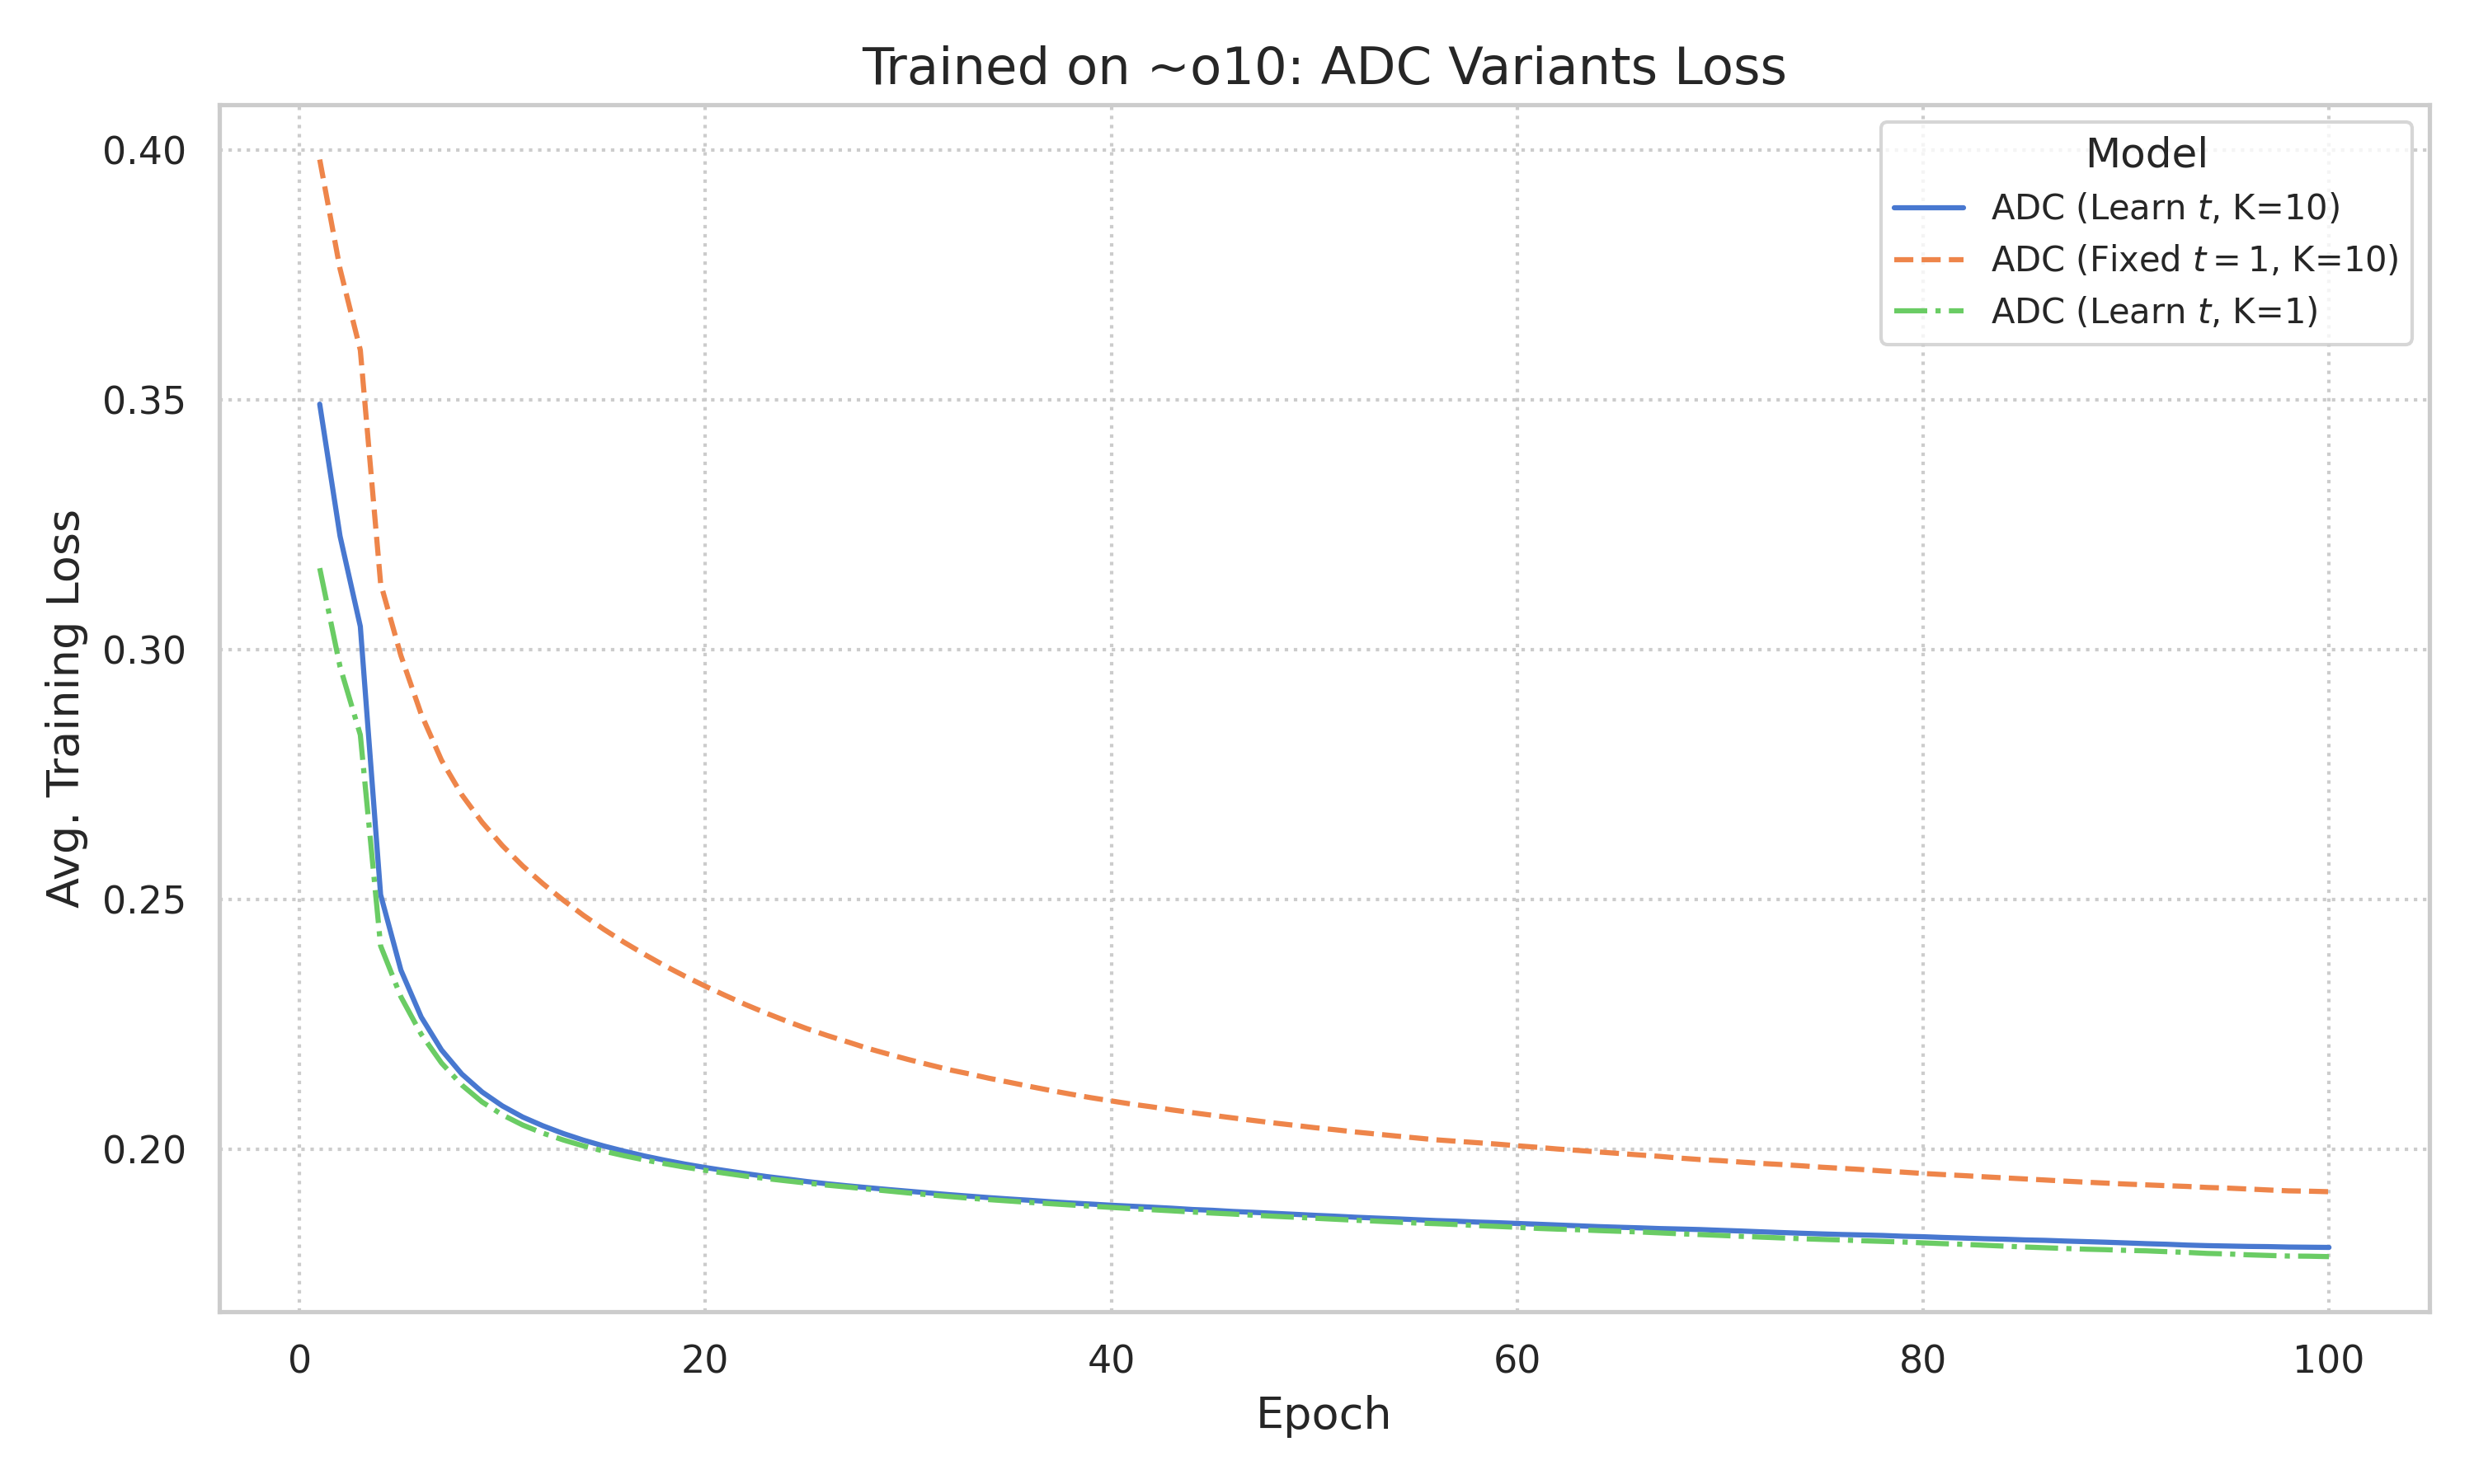
\includegraphics[width=\textwidth]{trainplotbase/TRAINED_ON_10_OBS/training_curves_focused/condition_o10/adc_variants_train_loss.png}
        \caption{ADC Variants: Training Loss}
        \label{fig:adc_train_loss_10obs}
    \end{subfigure}
    \hfill
    \begin{subfigure}[b]{0.48\textwidth}
        \centering
        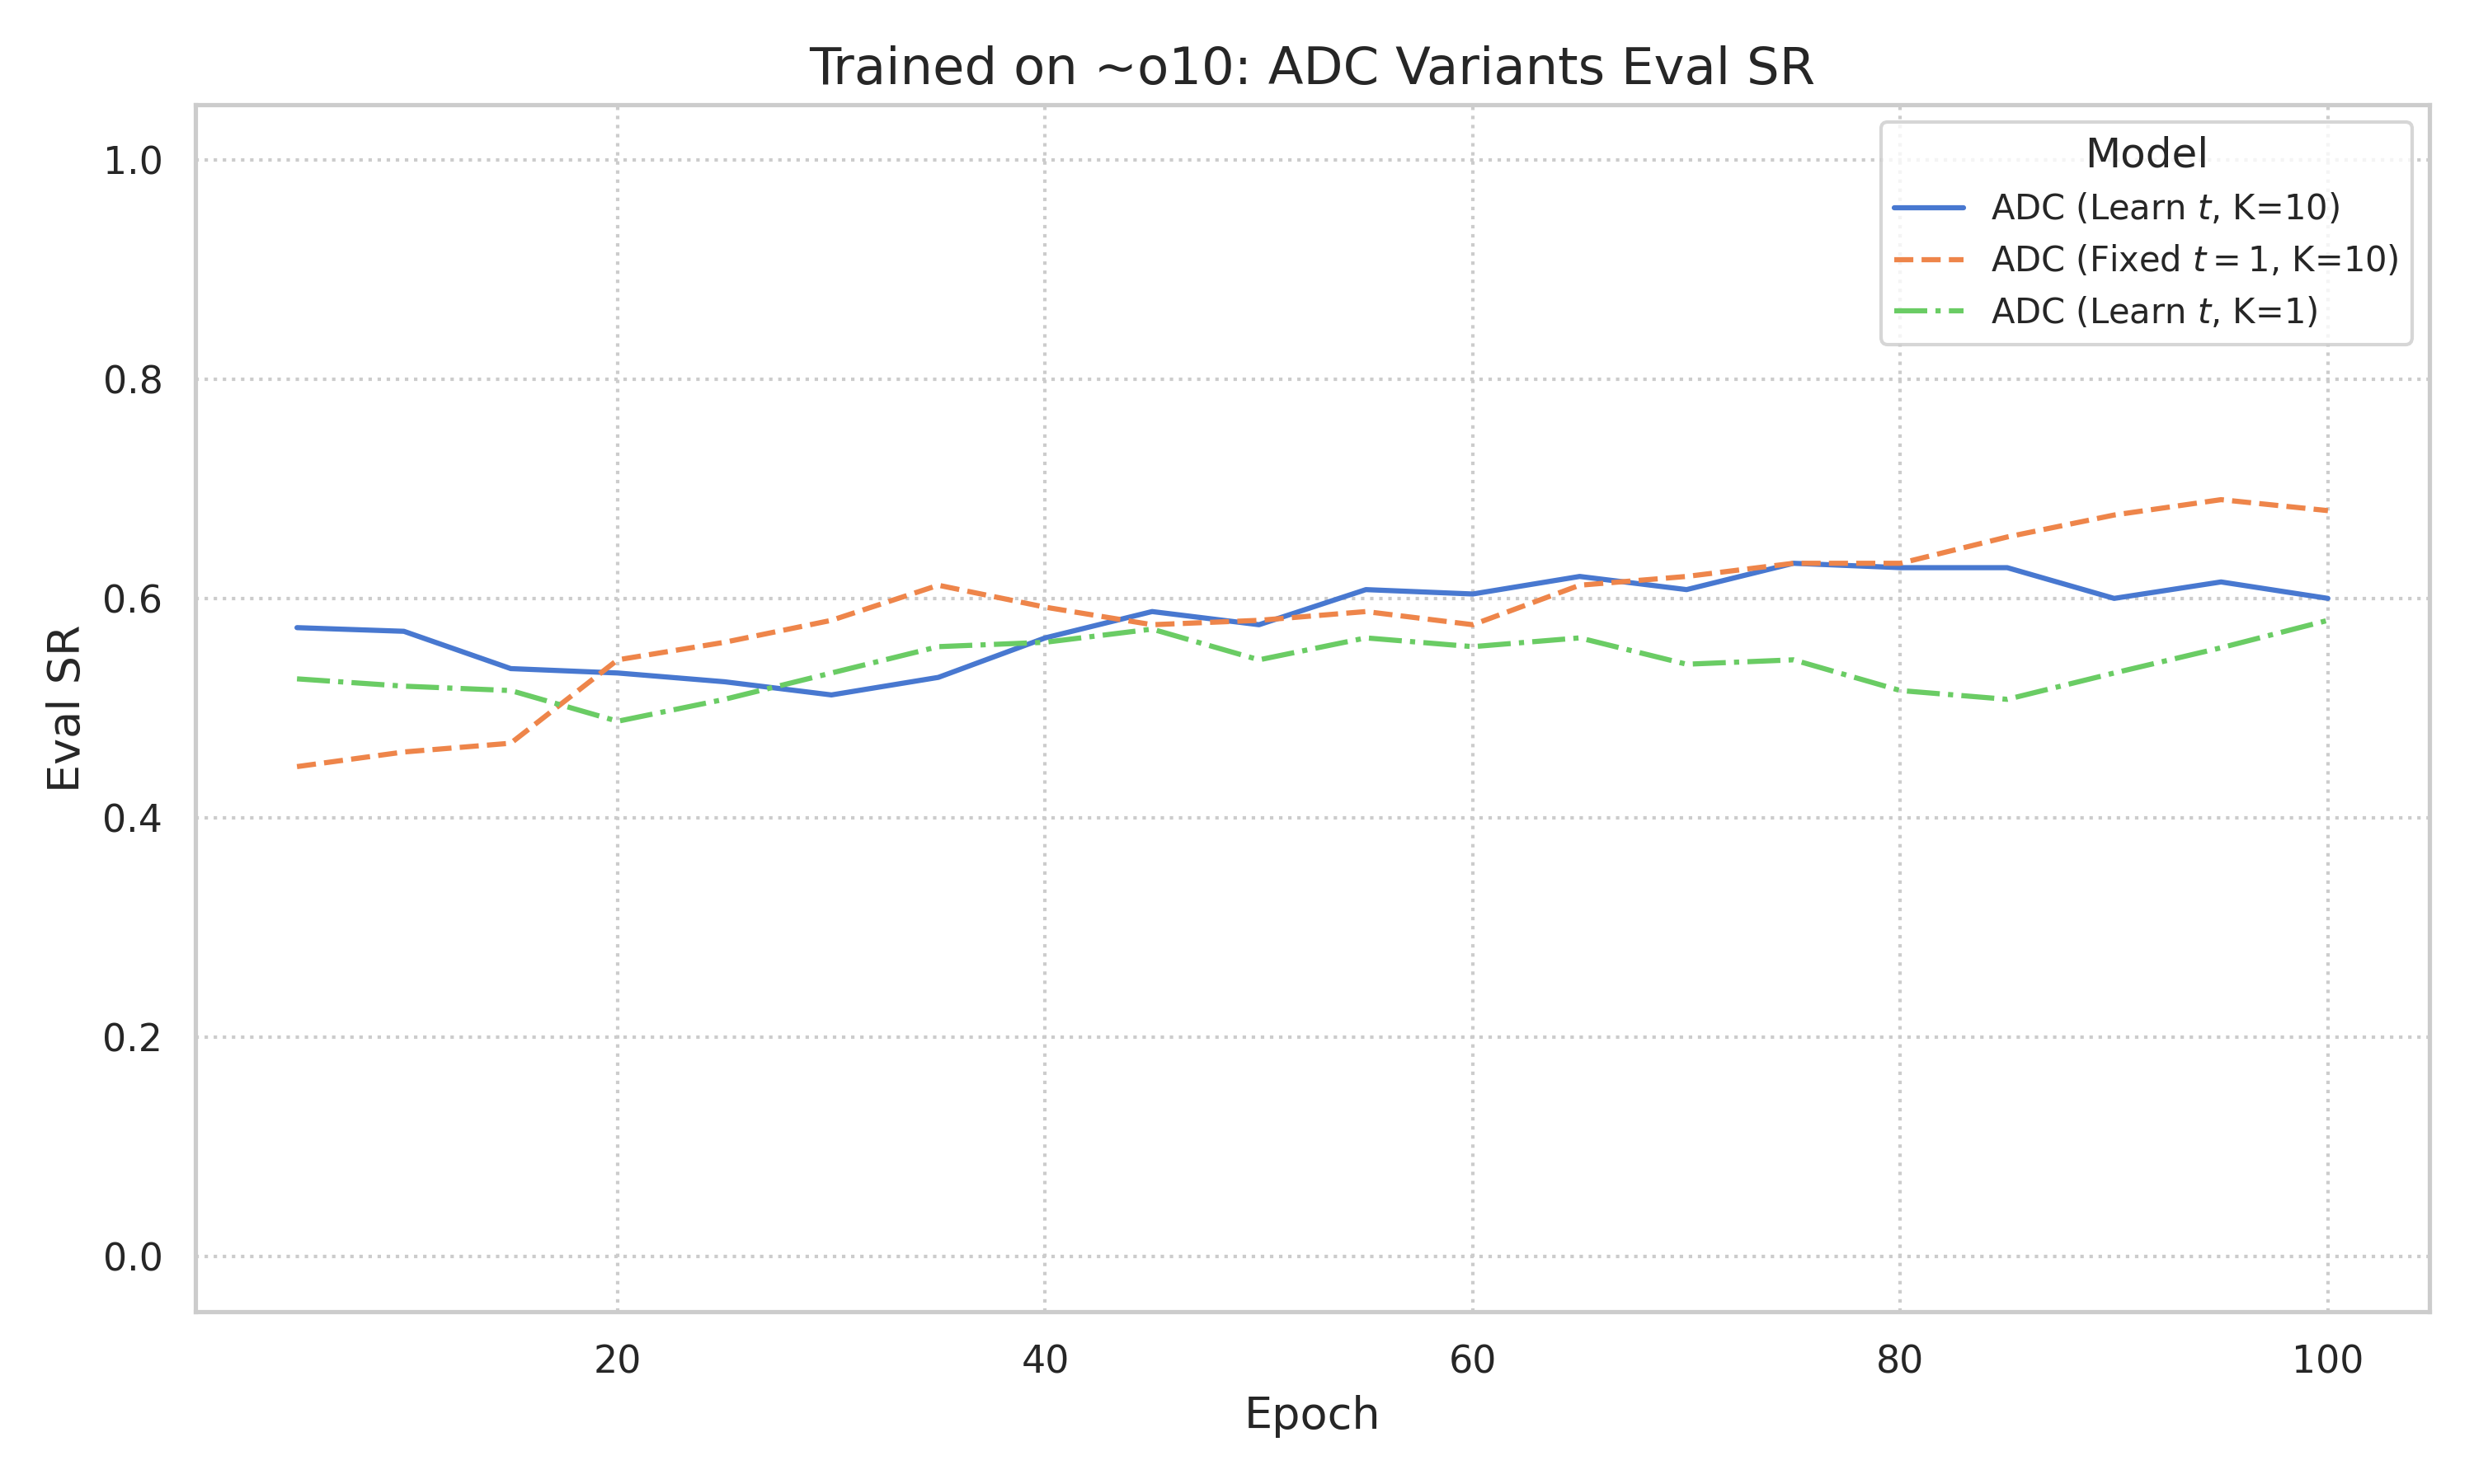
\includegraphics[width=\textwidth]{trainplotbase/TRAINED_ON_10_OBS/training_curves_focused/condition_o10/adc_variants_eval_sr.png}
        \caption{ADC Variants: Validation SR}
        \label{fig:adc_val_sr_10obs}
    \end{subfigure}

    \vspace{0.3cm} 

    % Row 2
    \begin{subfigure}[b]{0.48\textwidth}
        \centering
        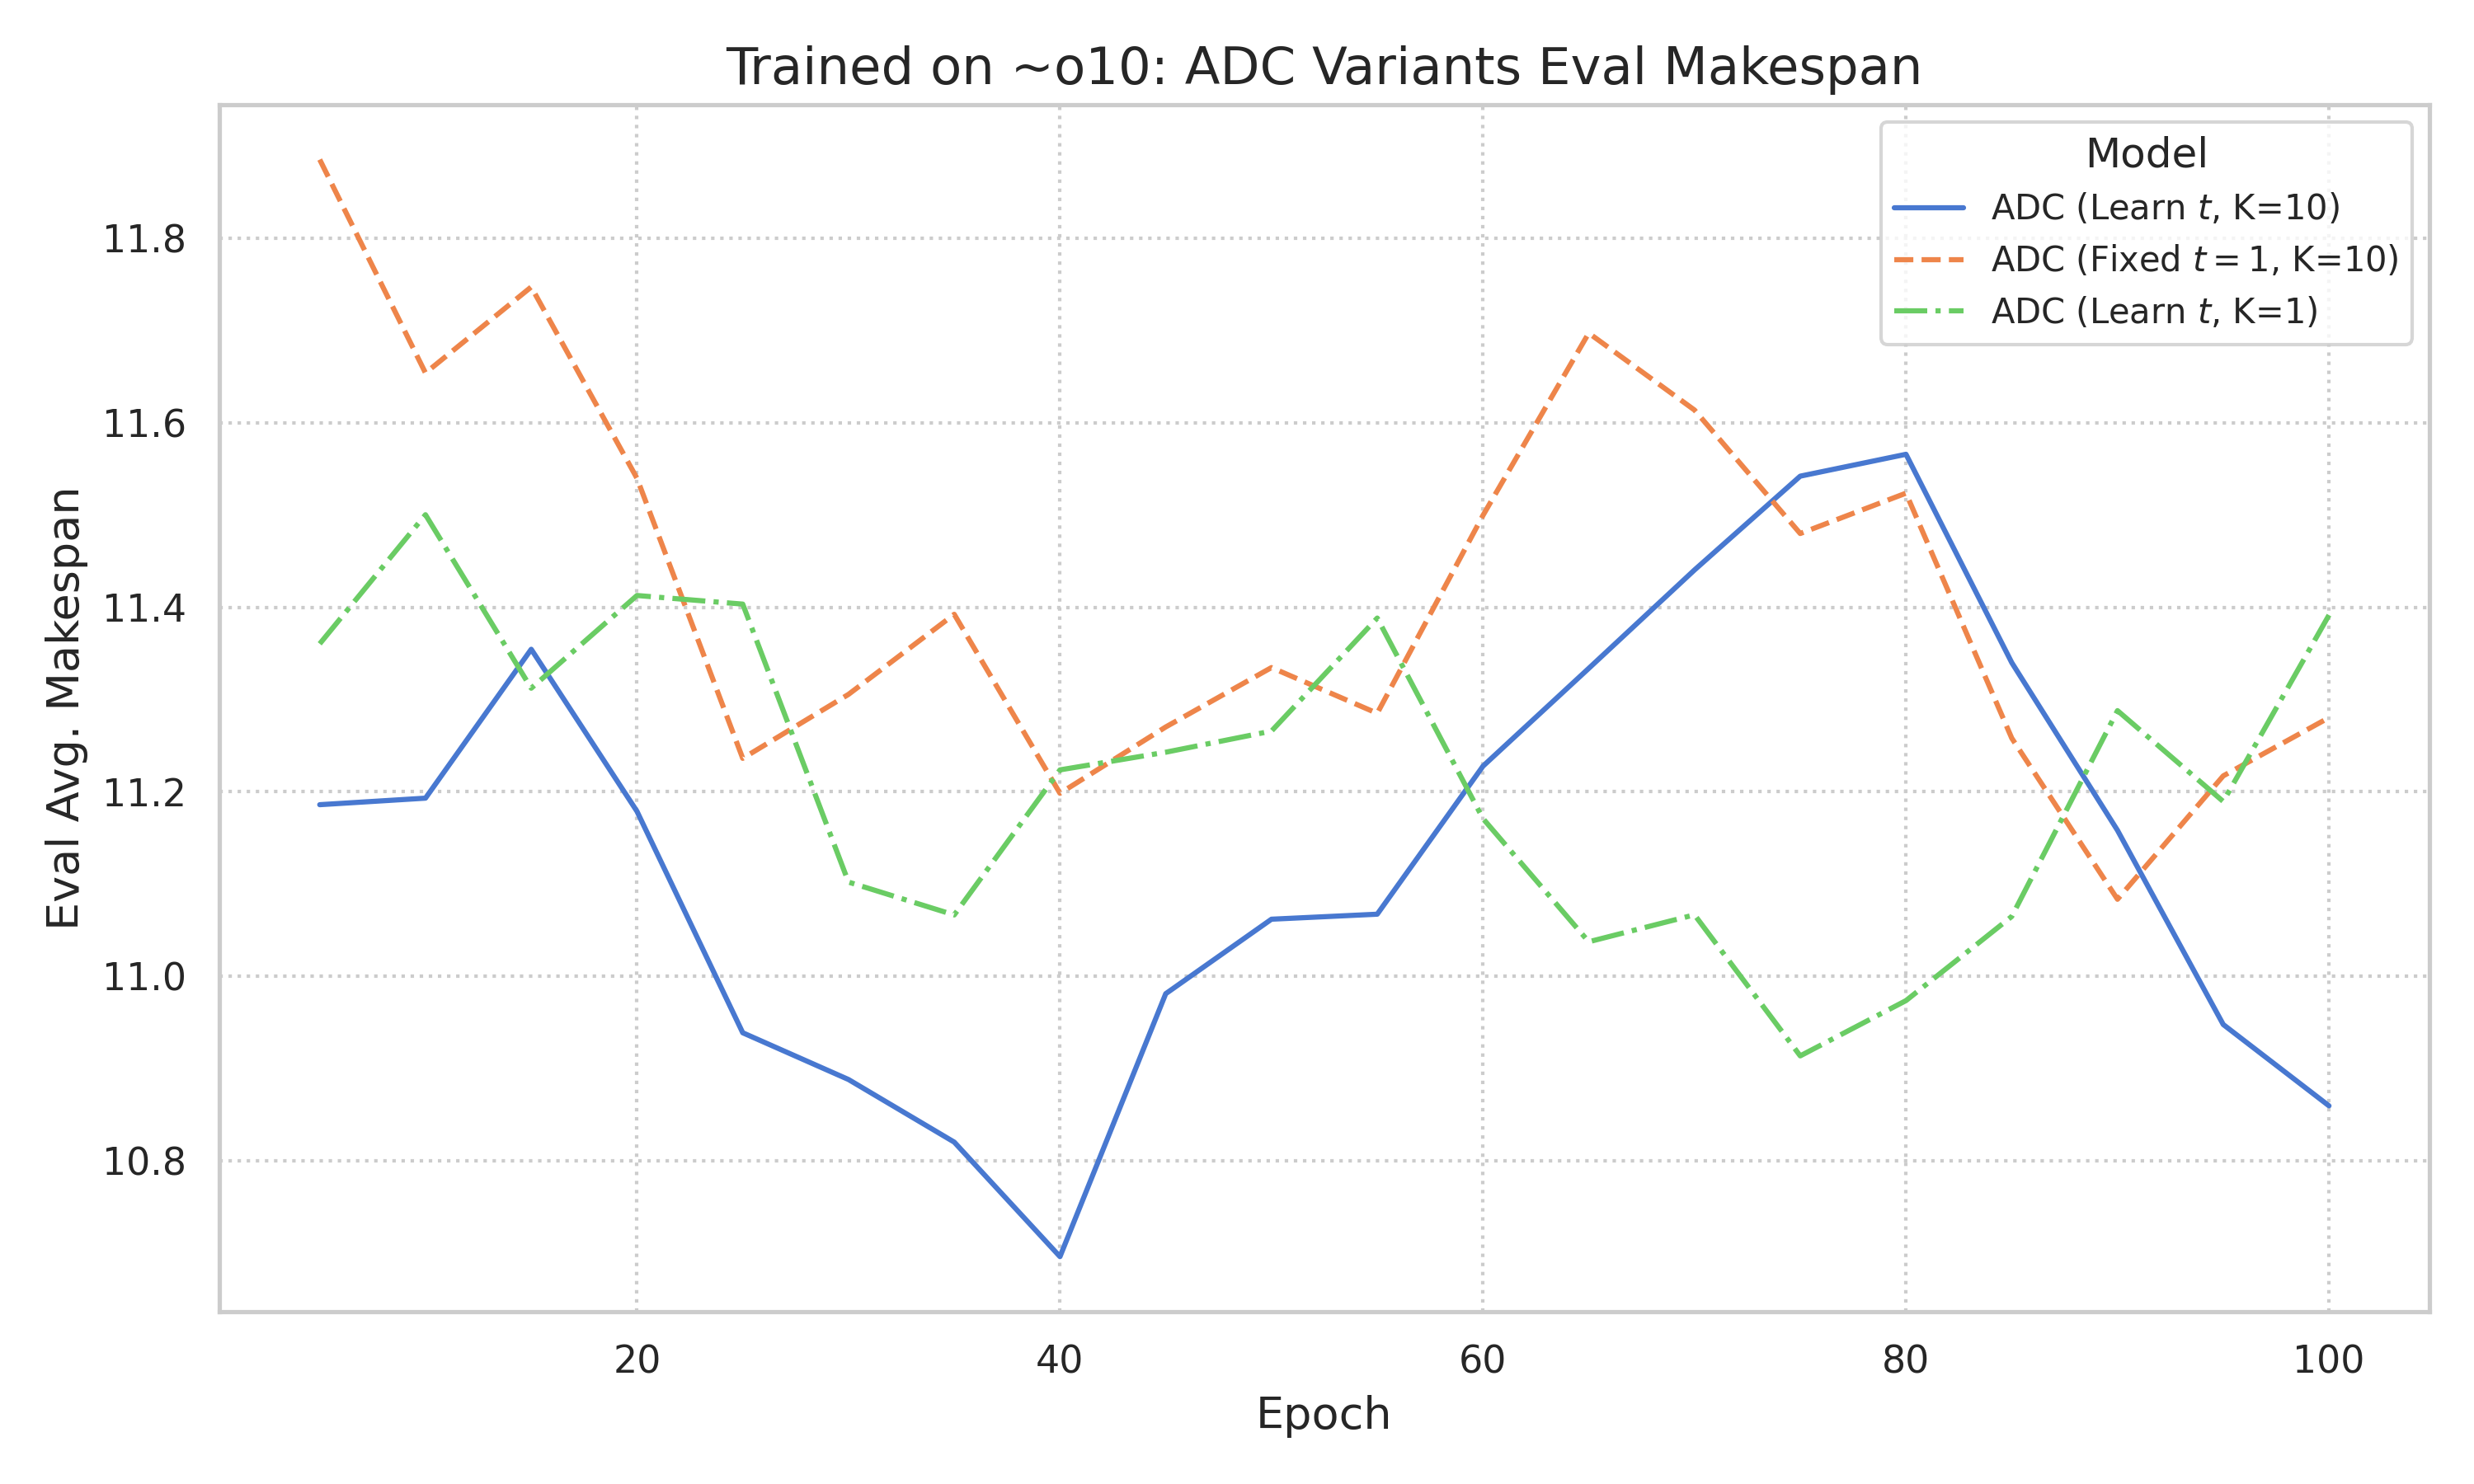
\includegraphics[width=\textwidth]{trainplotbase/TRAINED_ON_10_OBS/training_curves_focused/condition_o10/adc_variants_eval_am.png}
        \caption{ADC Variants: Validation AM}
        \label{fig:adc_val_am_10obs}
    \end{subfigure}
    \hfill
    \begin{subfigure}[b]{0.48\textwidth}
        \centering
        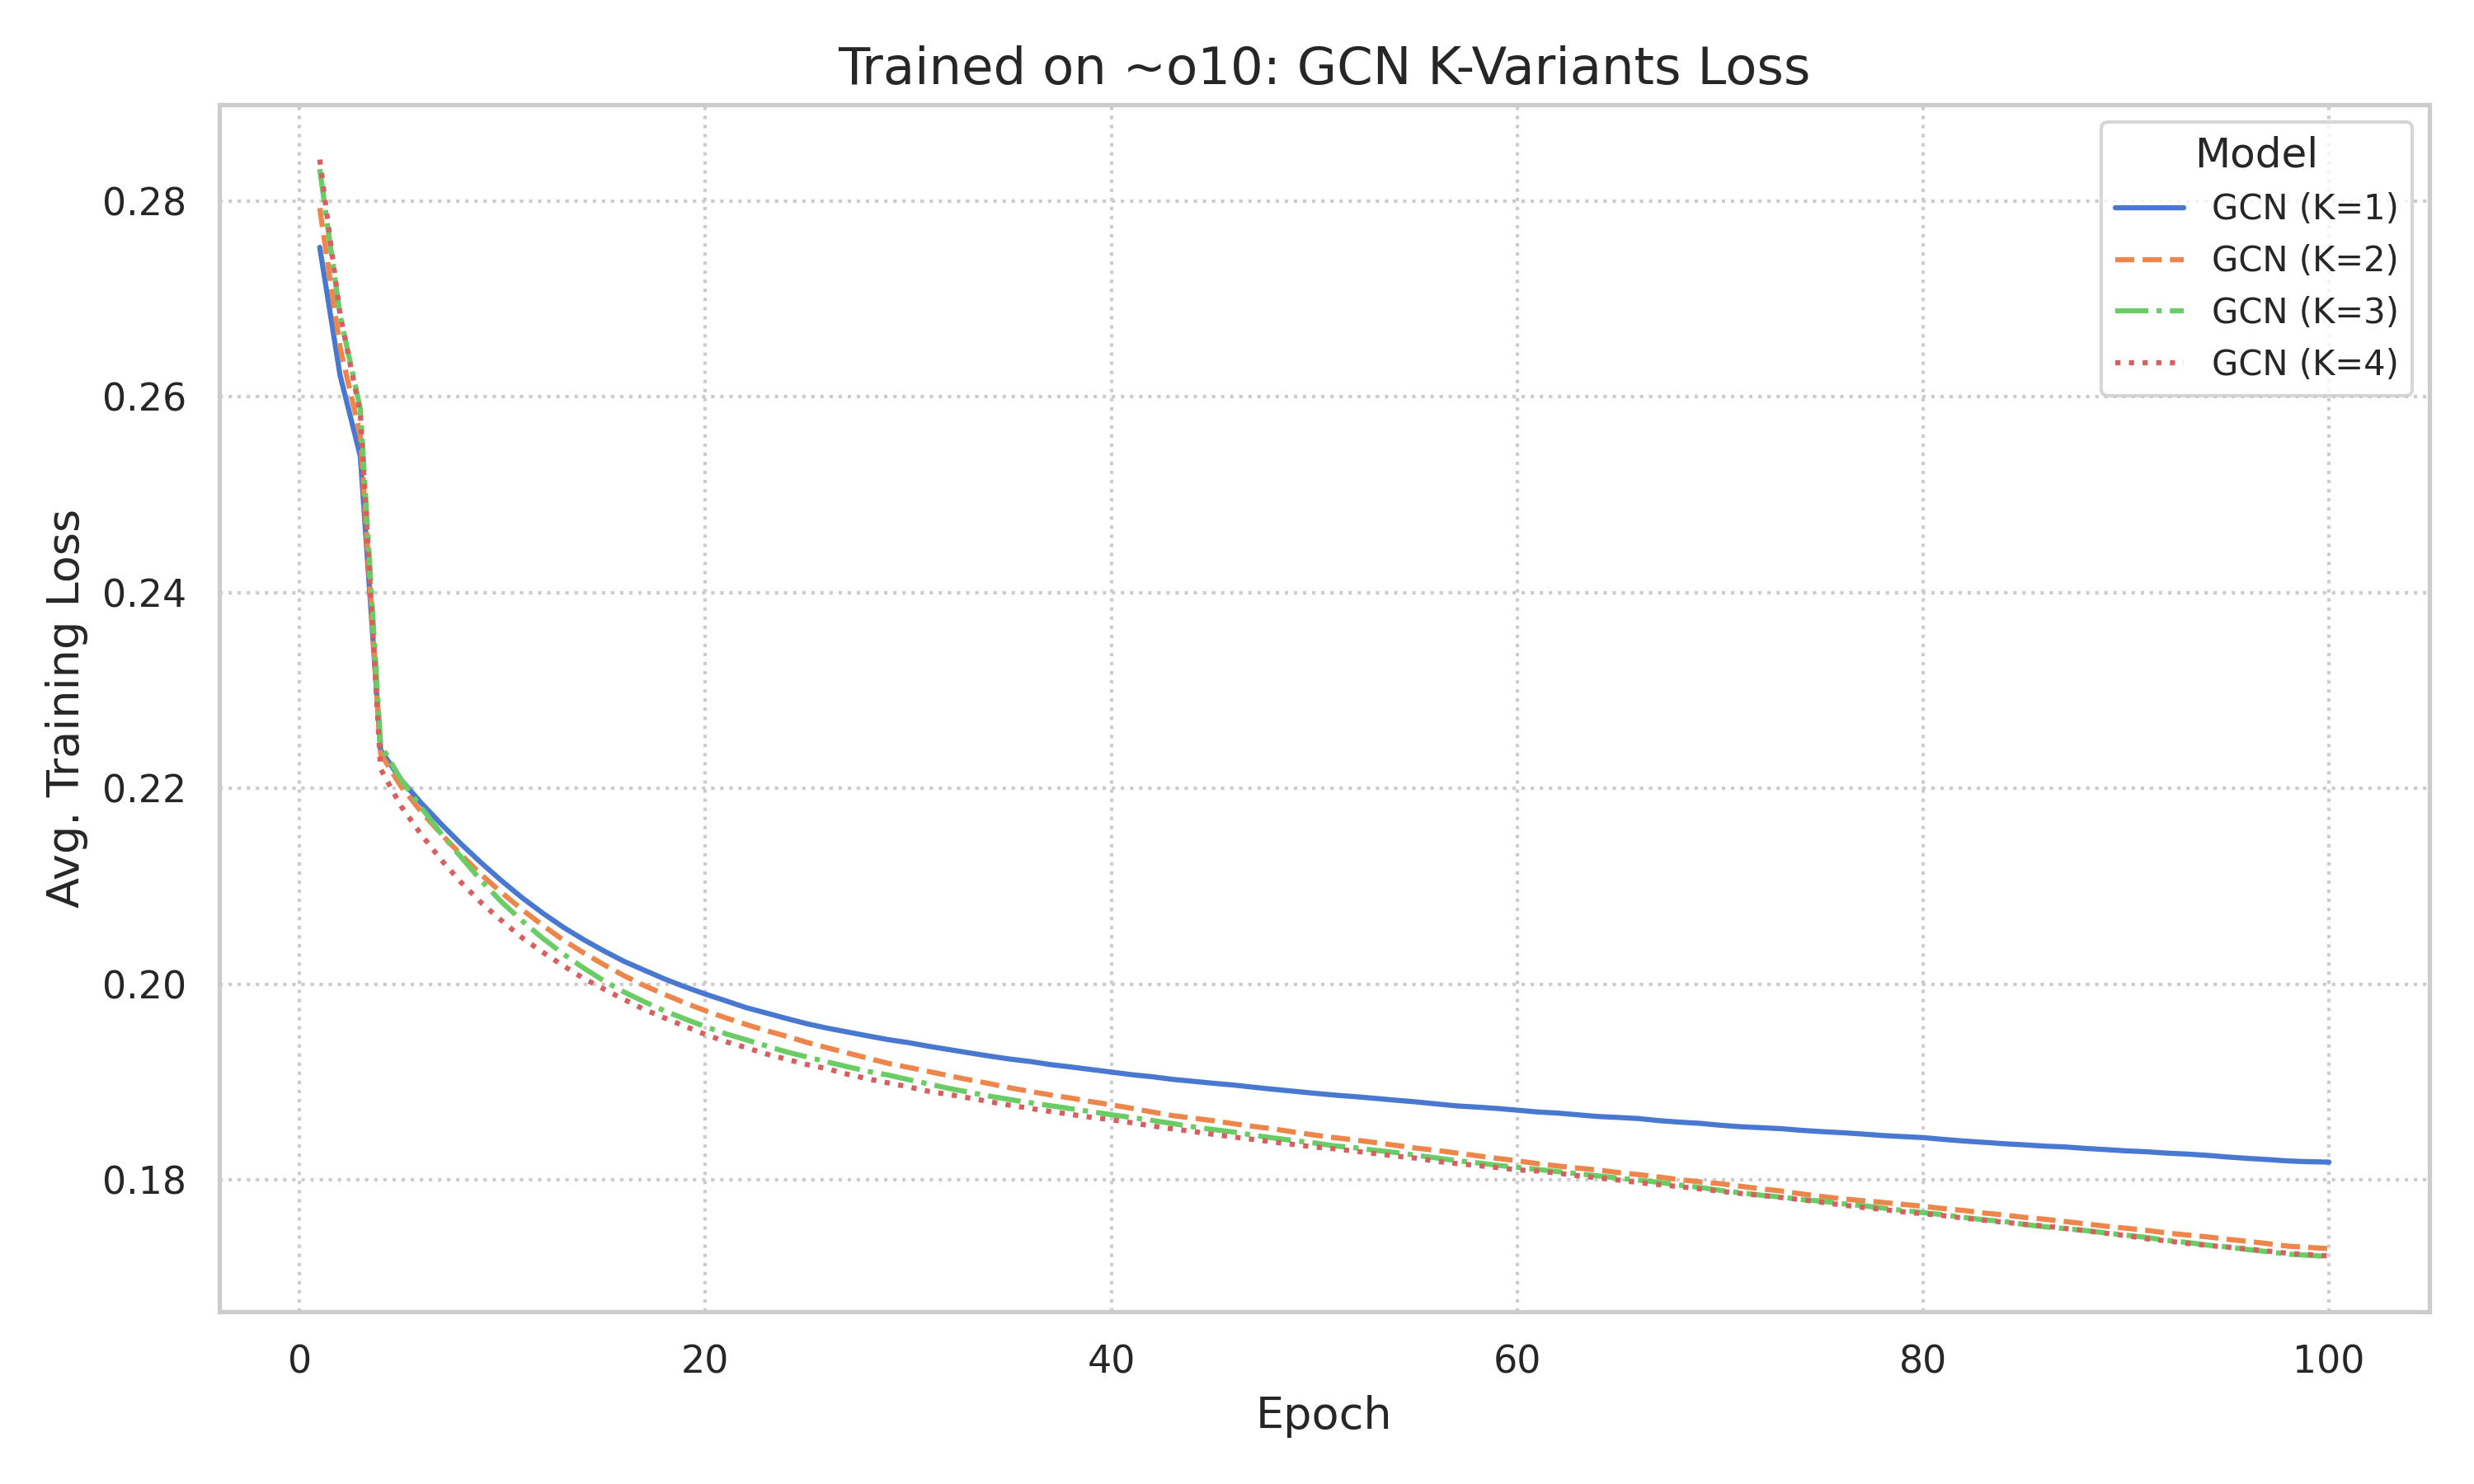
\includegraphics[width=\textwidth]{trainplotbase/TRAINED_ON_10_OBS/training_curves_focused/condition_o10/gcn_variants_train_loss.png}
        \caption{GCN Variants: Training Loss}
        \label{fig:gcn_train_loss_10obs}
    \end{subfigure}

    \vspace{0.3cm} 

    % Row 3
    \begin{subfigure}[b]{0.48\textwidth}
        \centering
        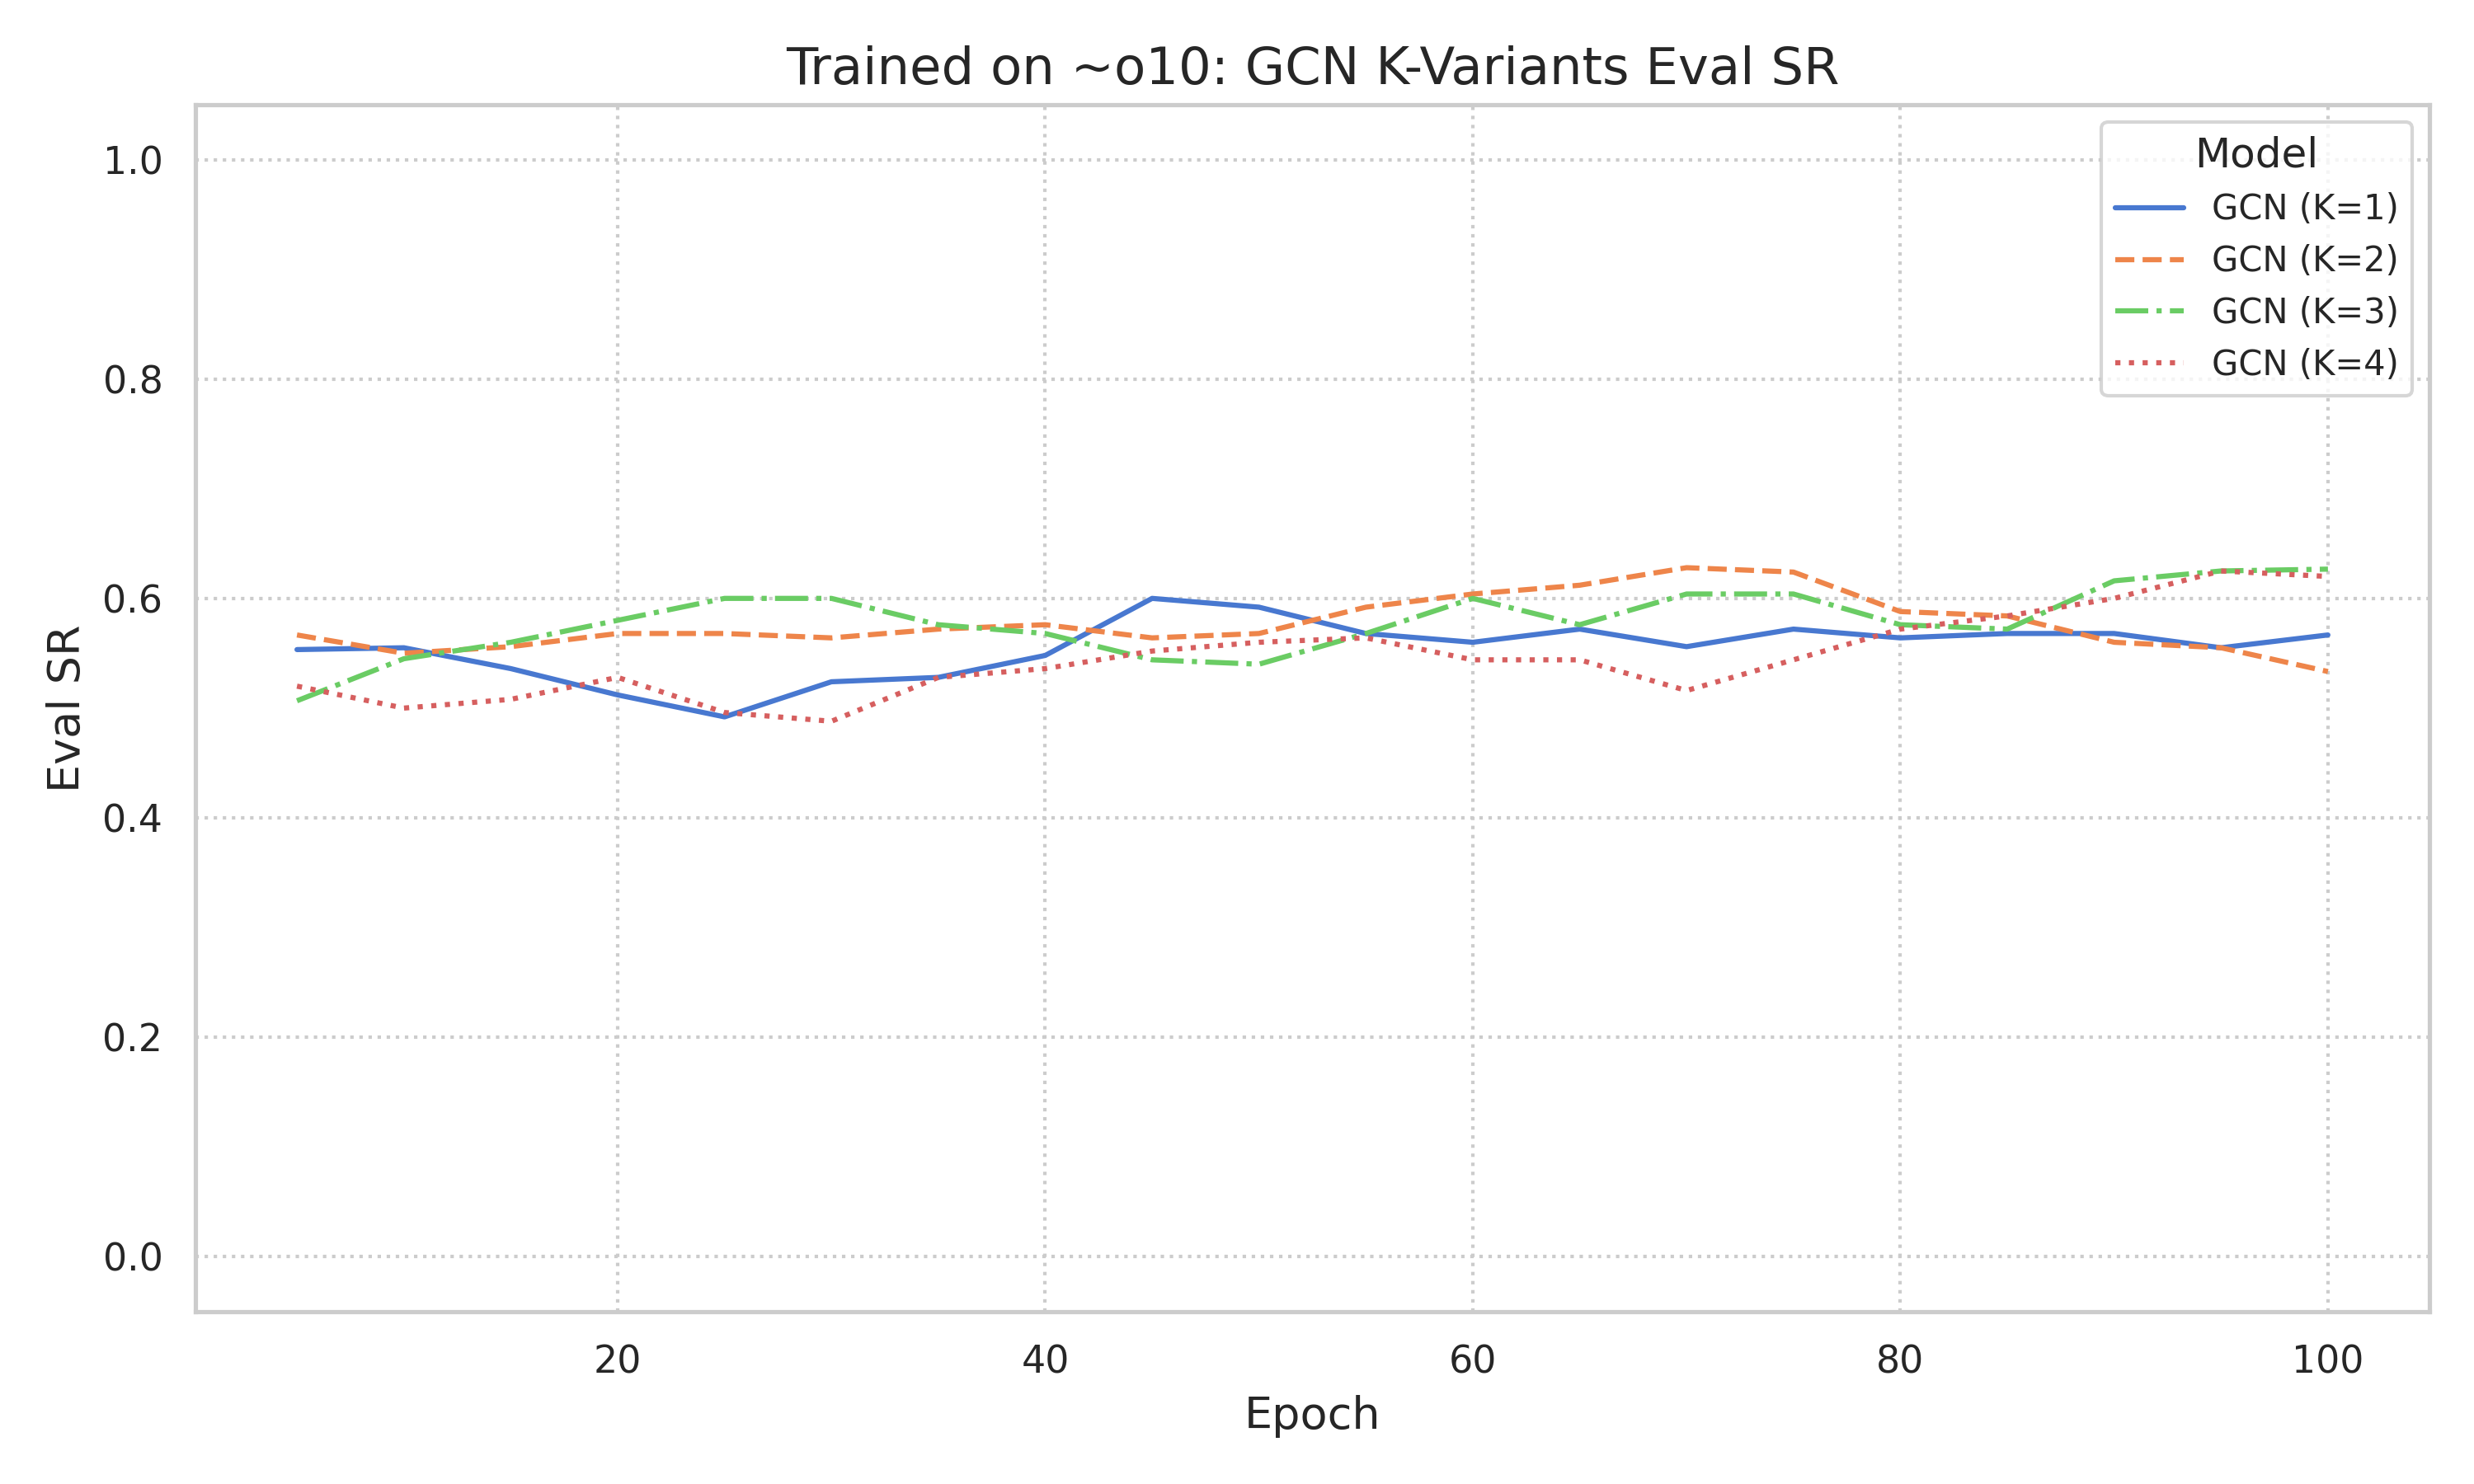
\includegraphics[width=\textwidth]{trainplotbase/TRAINED_ON_10_OBS/training_curves_focused/condition_o10/gcn_variants_eval_sr.png}
        \caption{GCN Variants: Validation SR}
        \label{fig:gcn_val_sr_10obs}
    \end{subfigure}
    \hfill
    \begin{subfigure}[b]{0.48\textwidth}
        \centering
        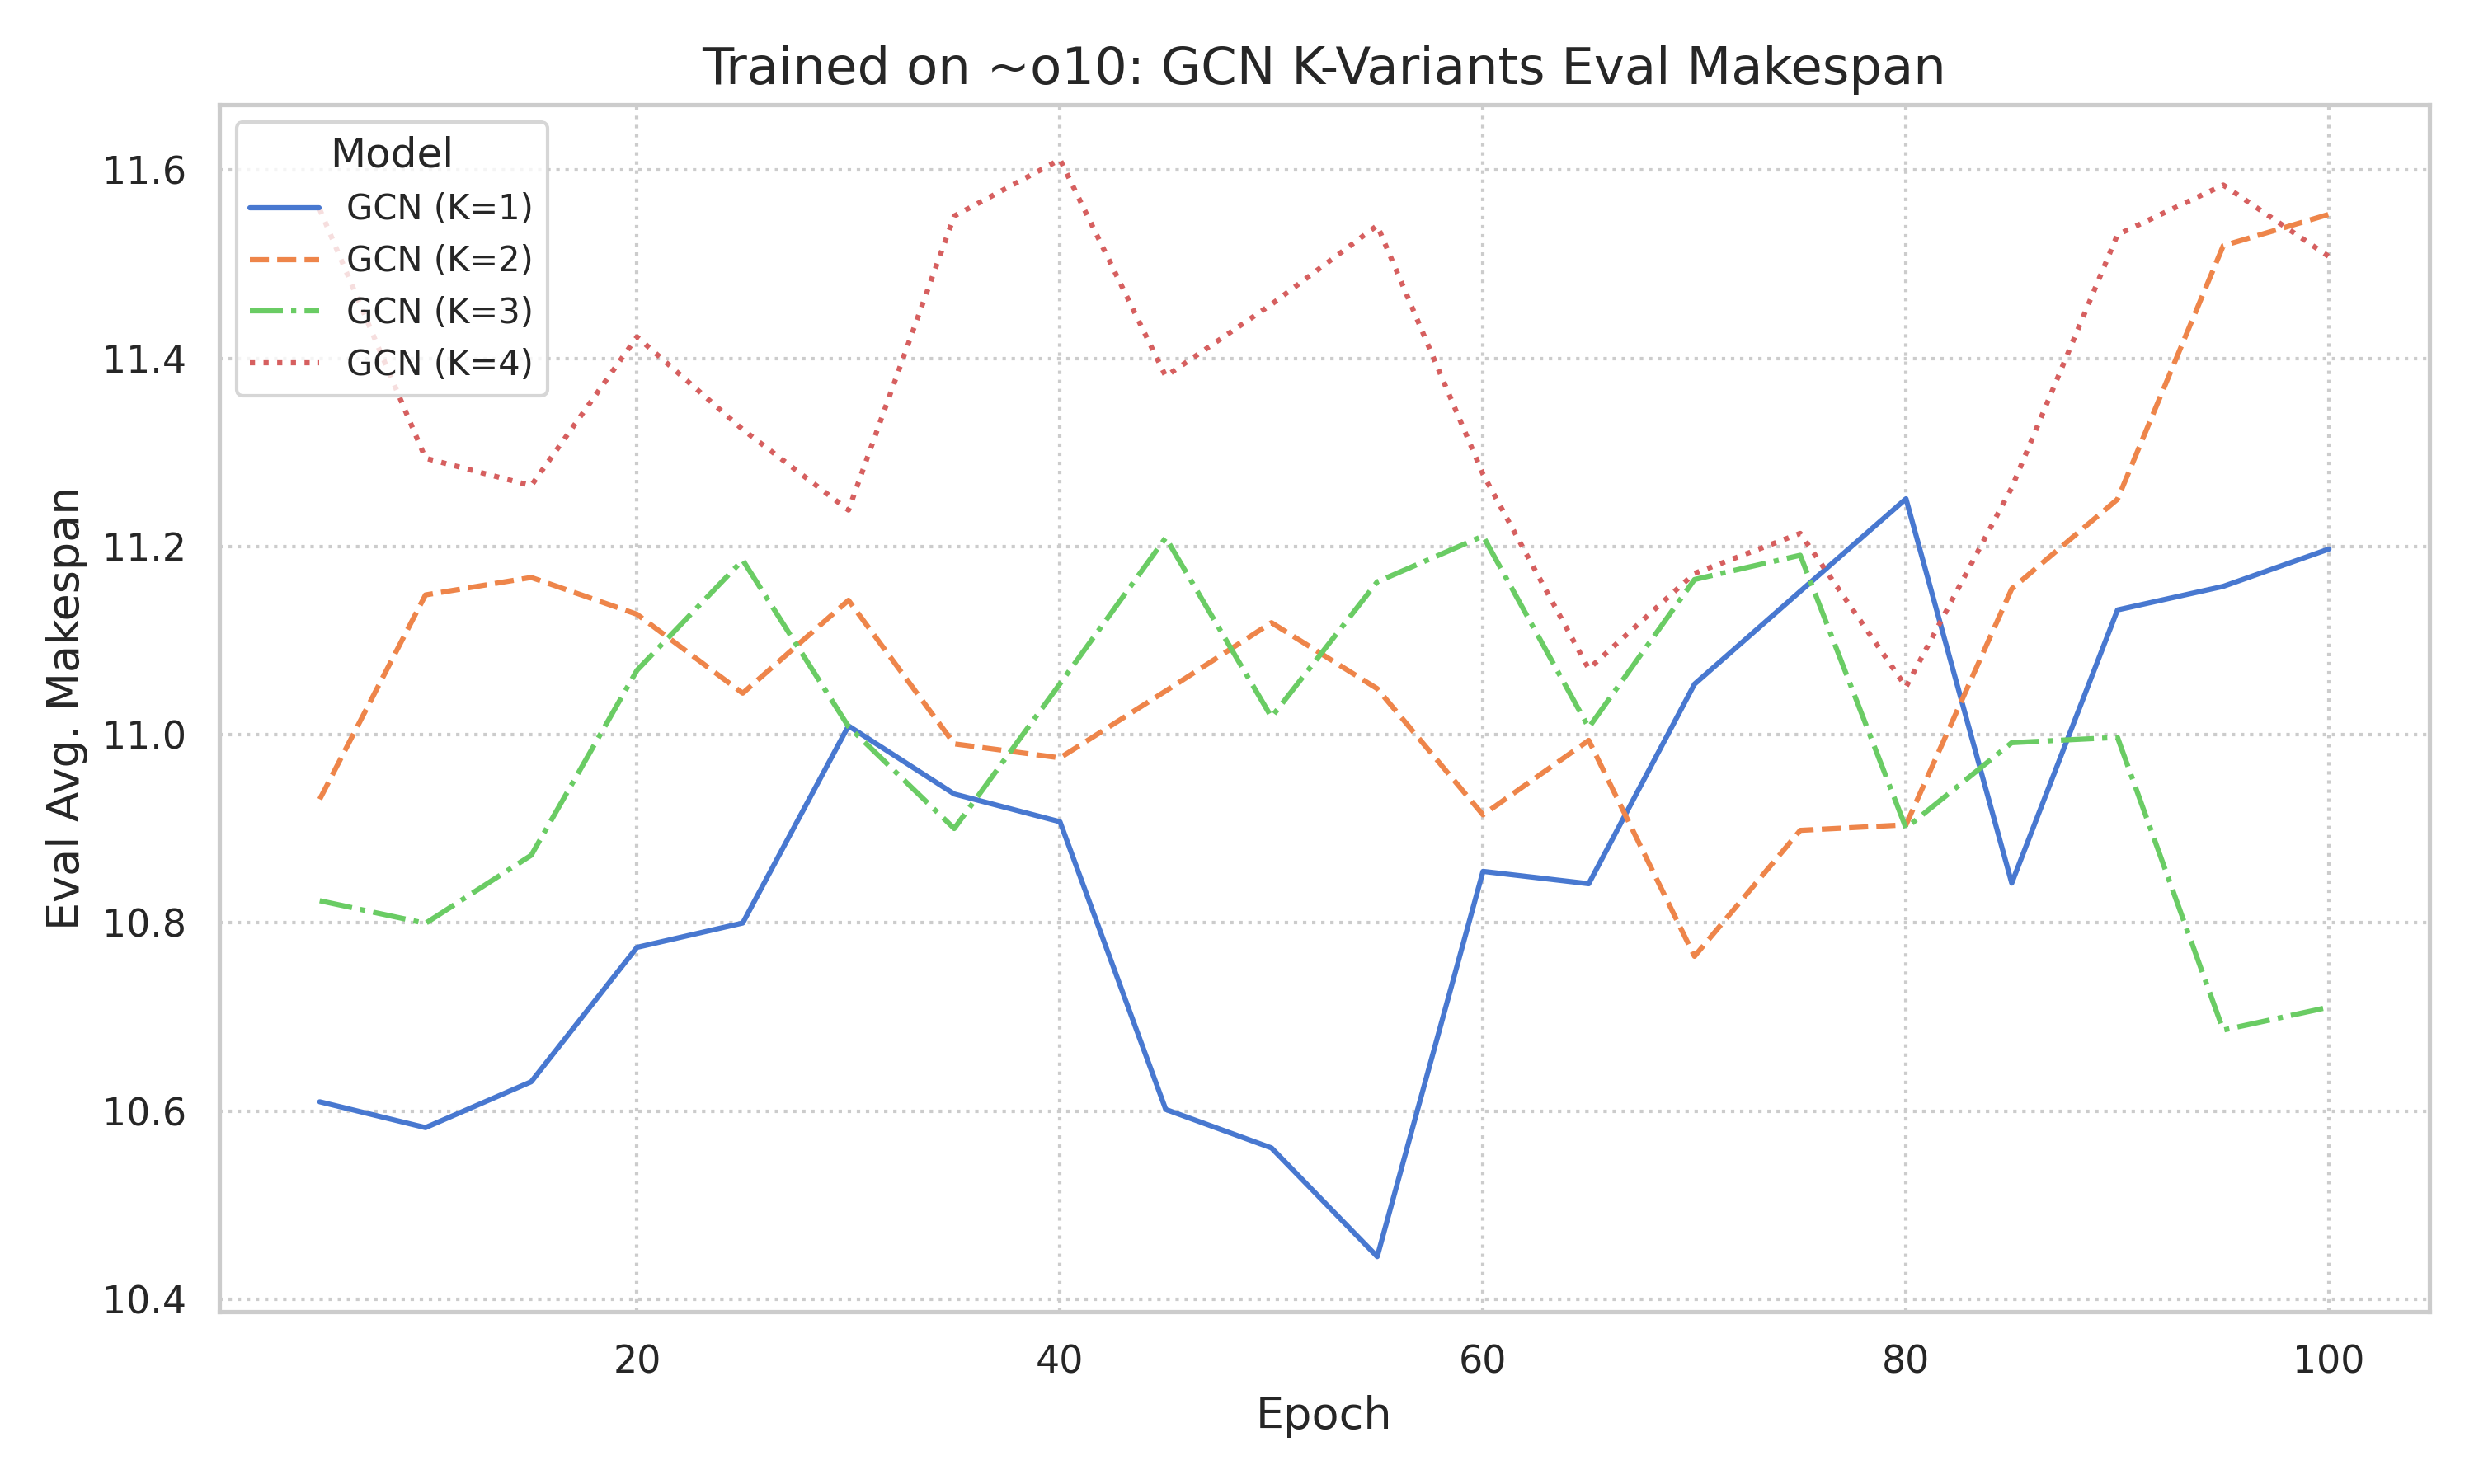
\includegraphics[width=\textwidth]{trainplotbase/TRAINED_ON_10_OBS/training_curves_focused/condition_o10/gcn_variants_eval_am.png}
        \caption{GCN Variants: Validation AM}
        \label{fig:gcn_val_am_10obs}
    \end{subfigure}

    \caption{Training progress for models trained on the 10\% obstacle density dataset. The plots display: (a) ADC Training Loss, (b) ADC Validation SR, (c) ADC Validation AM, (d) GCN Training Loss, (e) GCN Validation SR, and (f) GCN Validation AM. }
    \label{fig:training_curves_10obs_improved}
\end{figure}
\newpage

\subsection{Training on 20\% Obstacle Density Dataset}
\label{subsec:training_20obs}
The training procedure was repeated for models using the dataset generated with 20\% obstacle density. The corresponding training curves are presented in Figure~\ref{fig:training_curves_20obs_improved}.

\begin{figure}[htbp]
    \centering
    % ADC Variants - Trained on 20% Obstacles
    \begin{subfigure}[b]{0.48\textwidth}
        \centering
        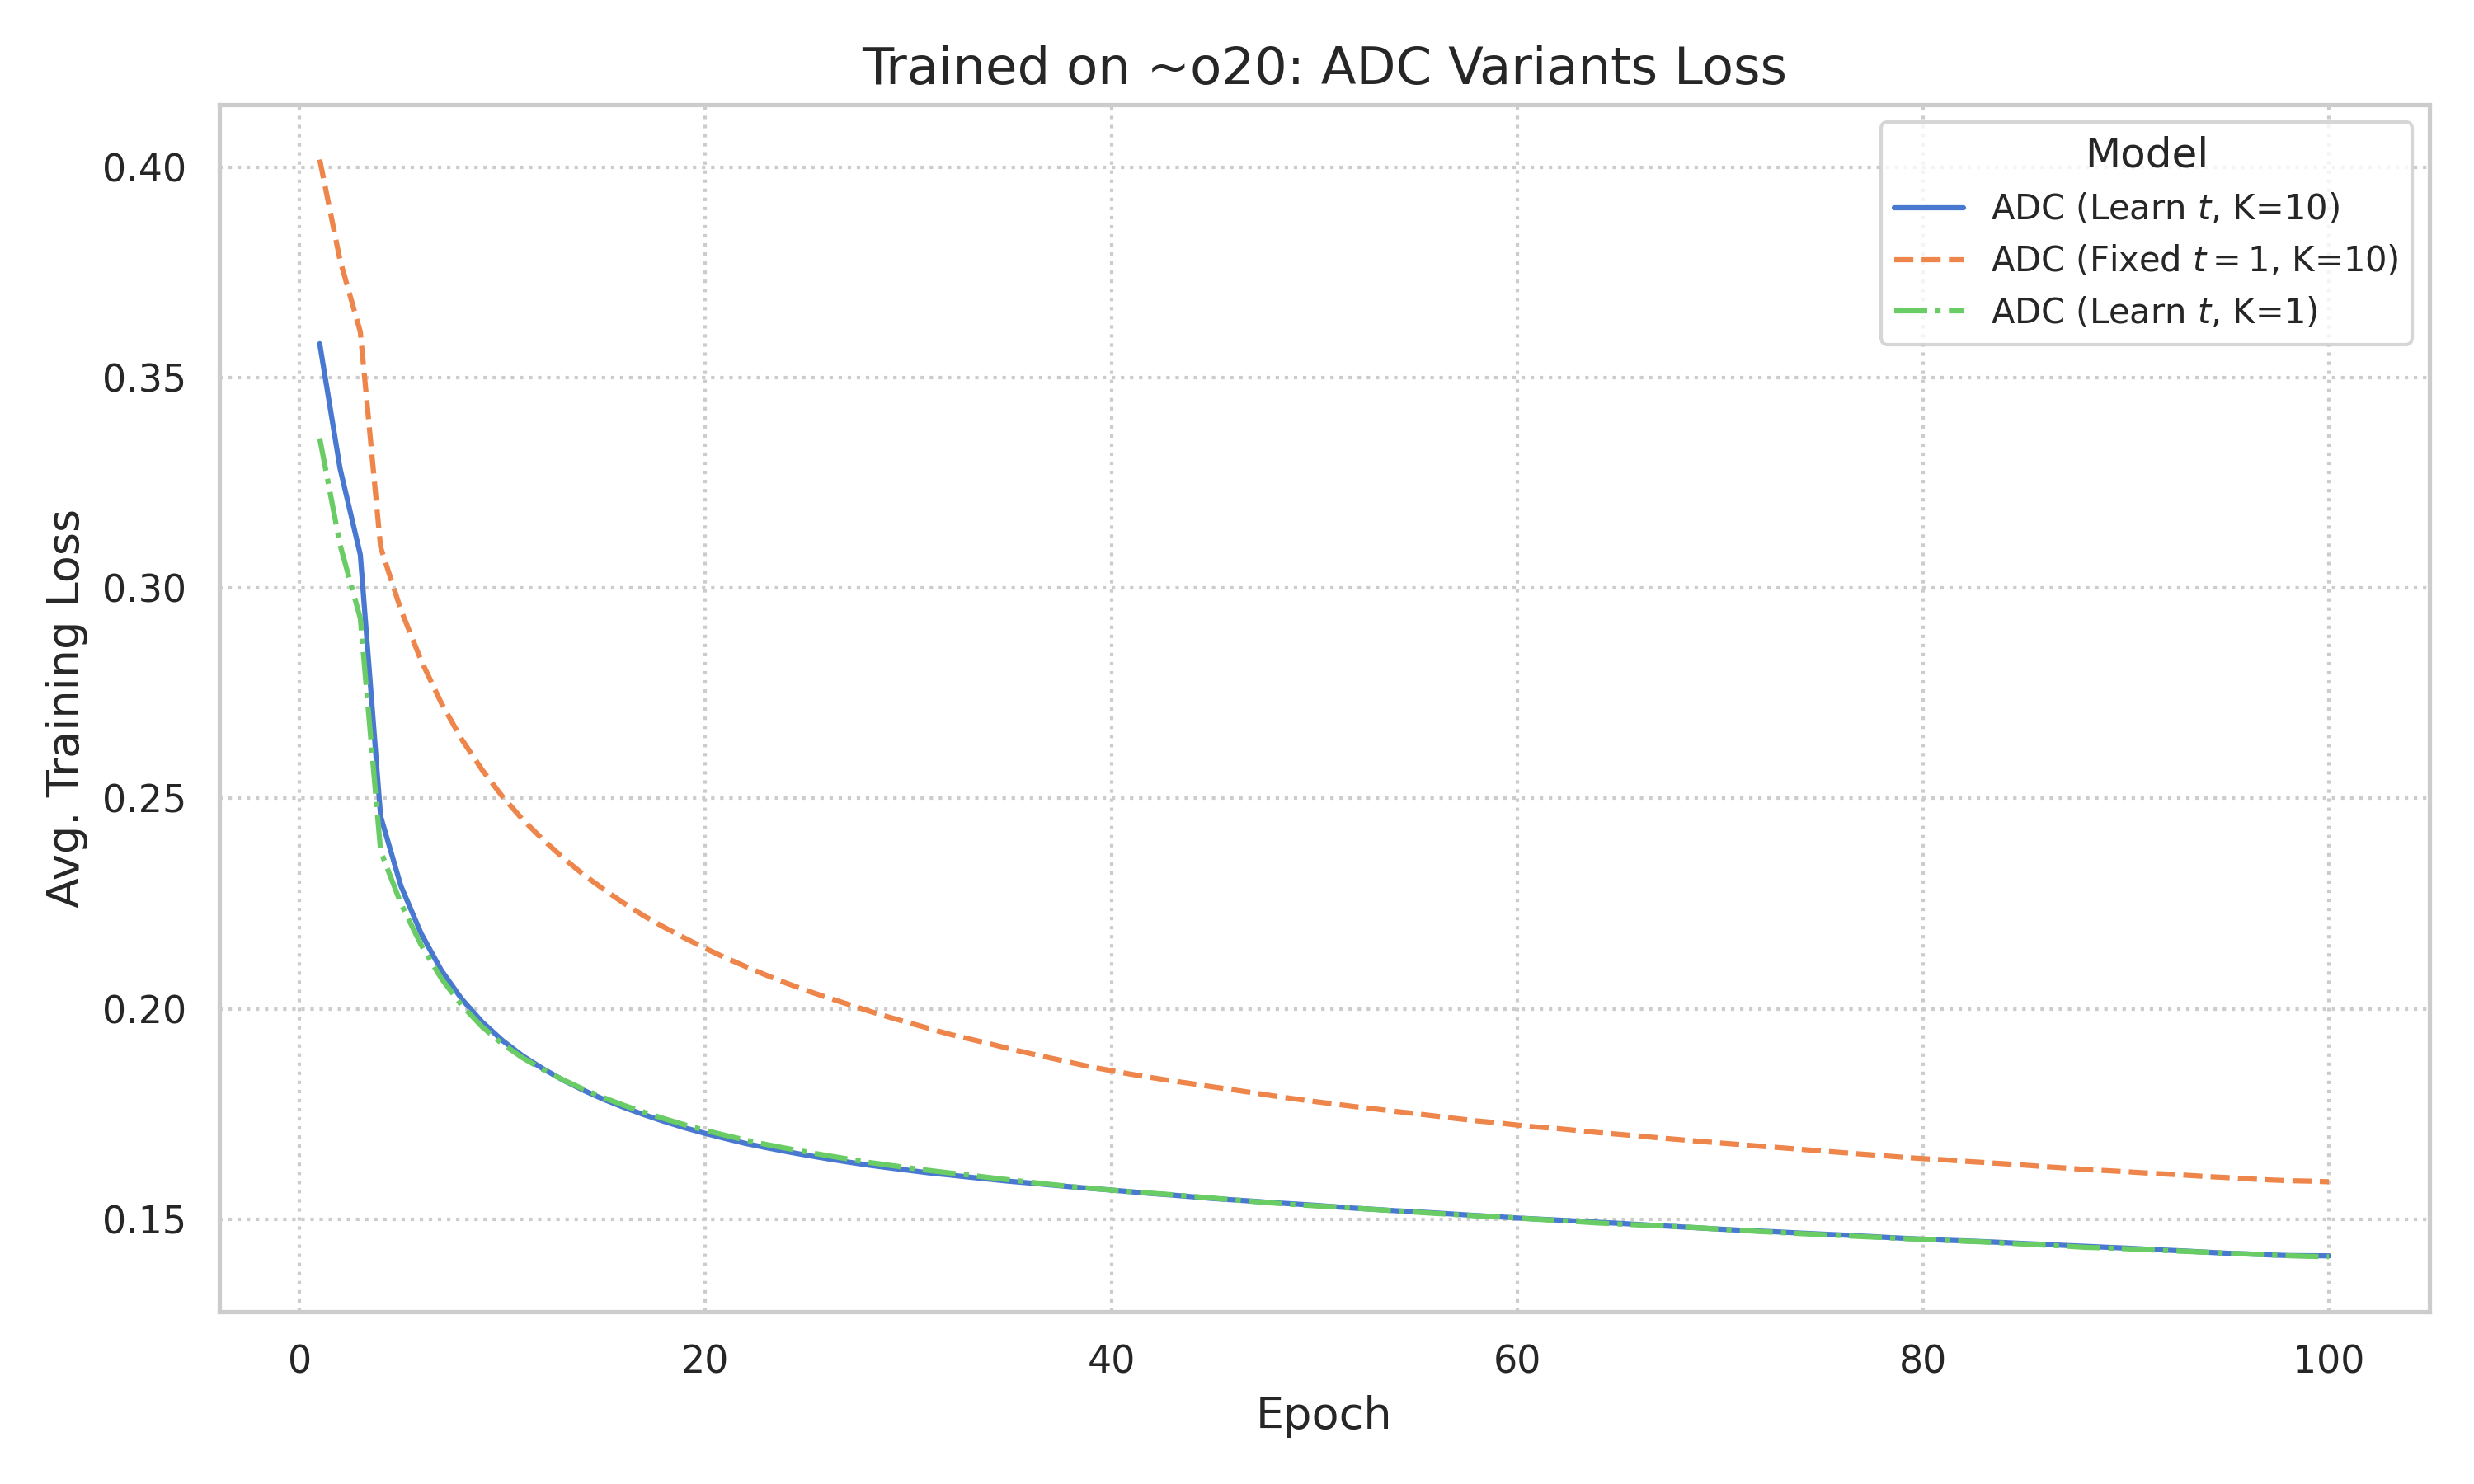
\includegraphics[width=\textwidth]{trainplotbase/TRAINED_ON_20_OBS/training_curves_focused/condition_o20/adc_variants_train_loss.png} % UPDATE PATH
        \caption{ADC Variants: Training Loss (20\% Obst.)}
        \label{fig:adc_train_loss_20obs}
    \end{subfigure}
    \hfill
    \begin{subfigure}[b]{0.48\textwidth}
        \centering
        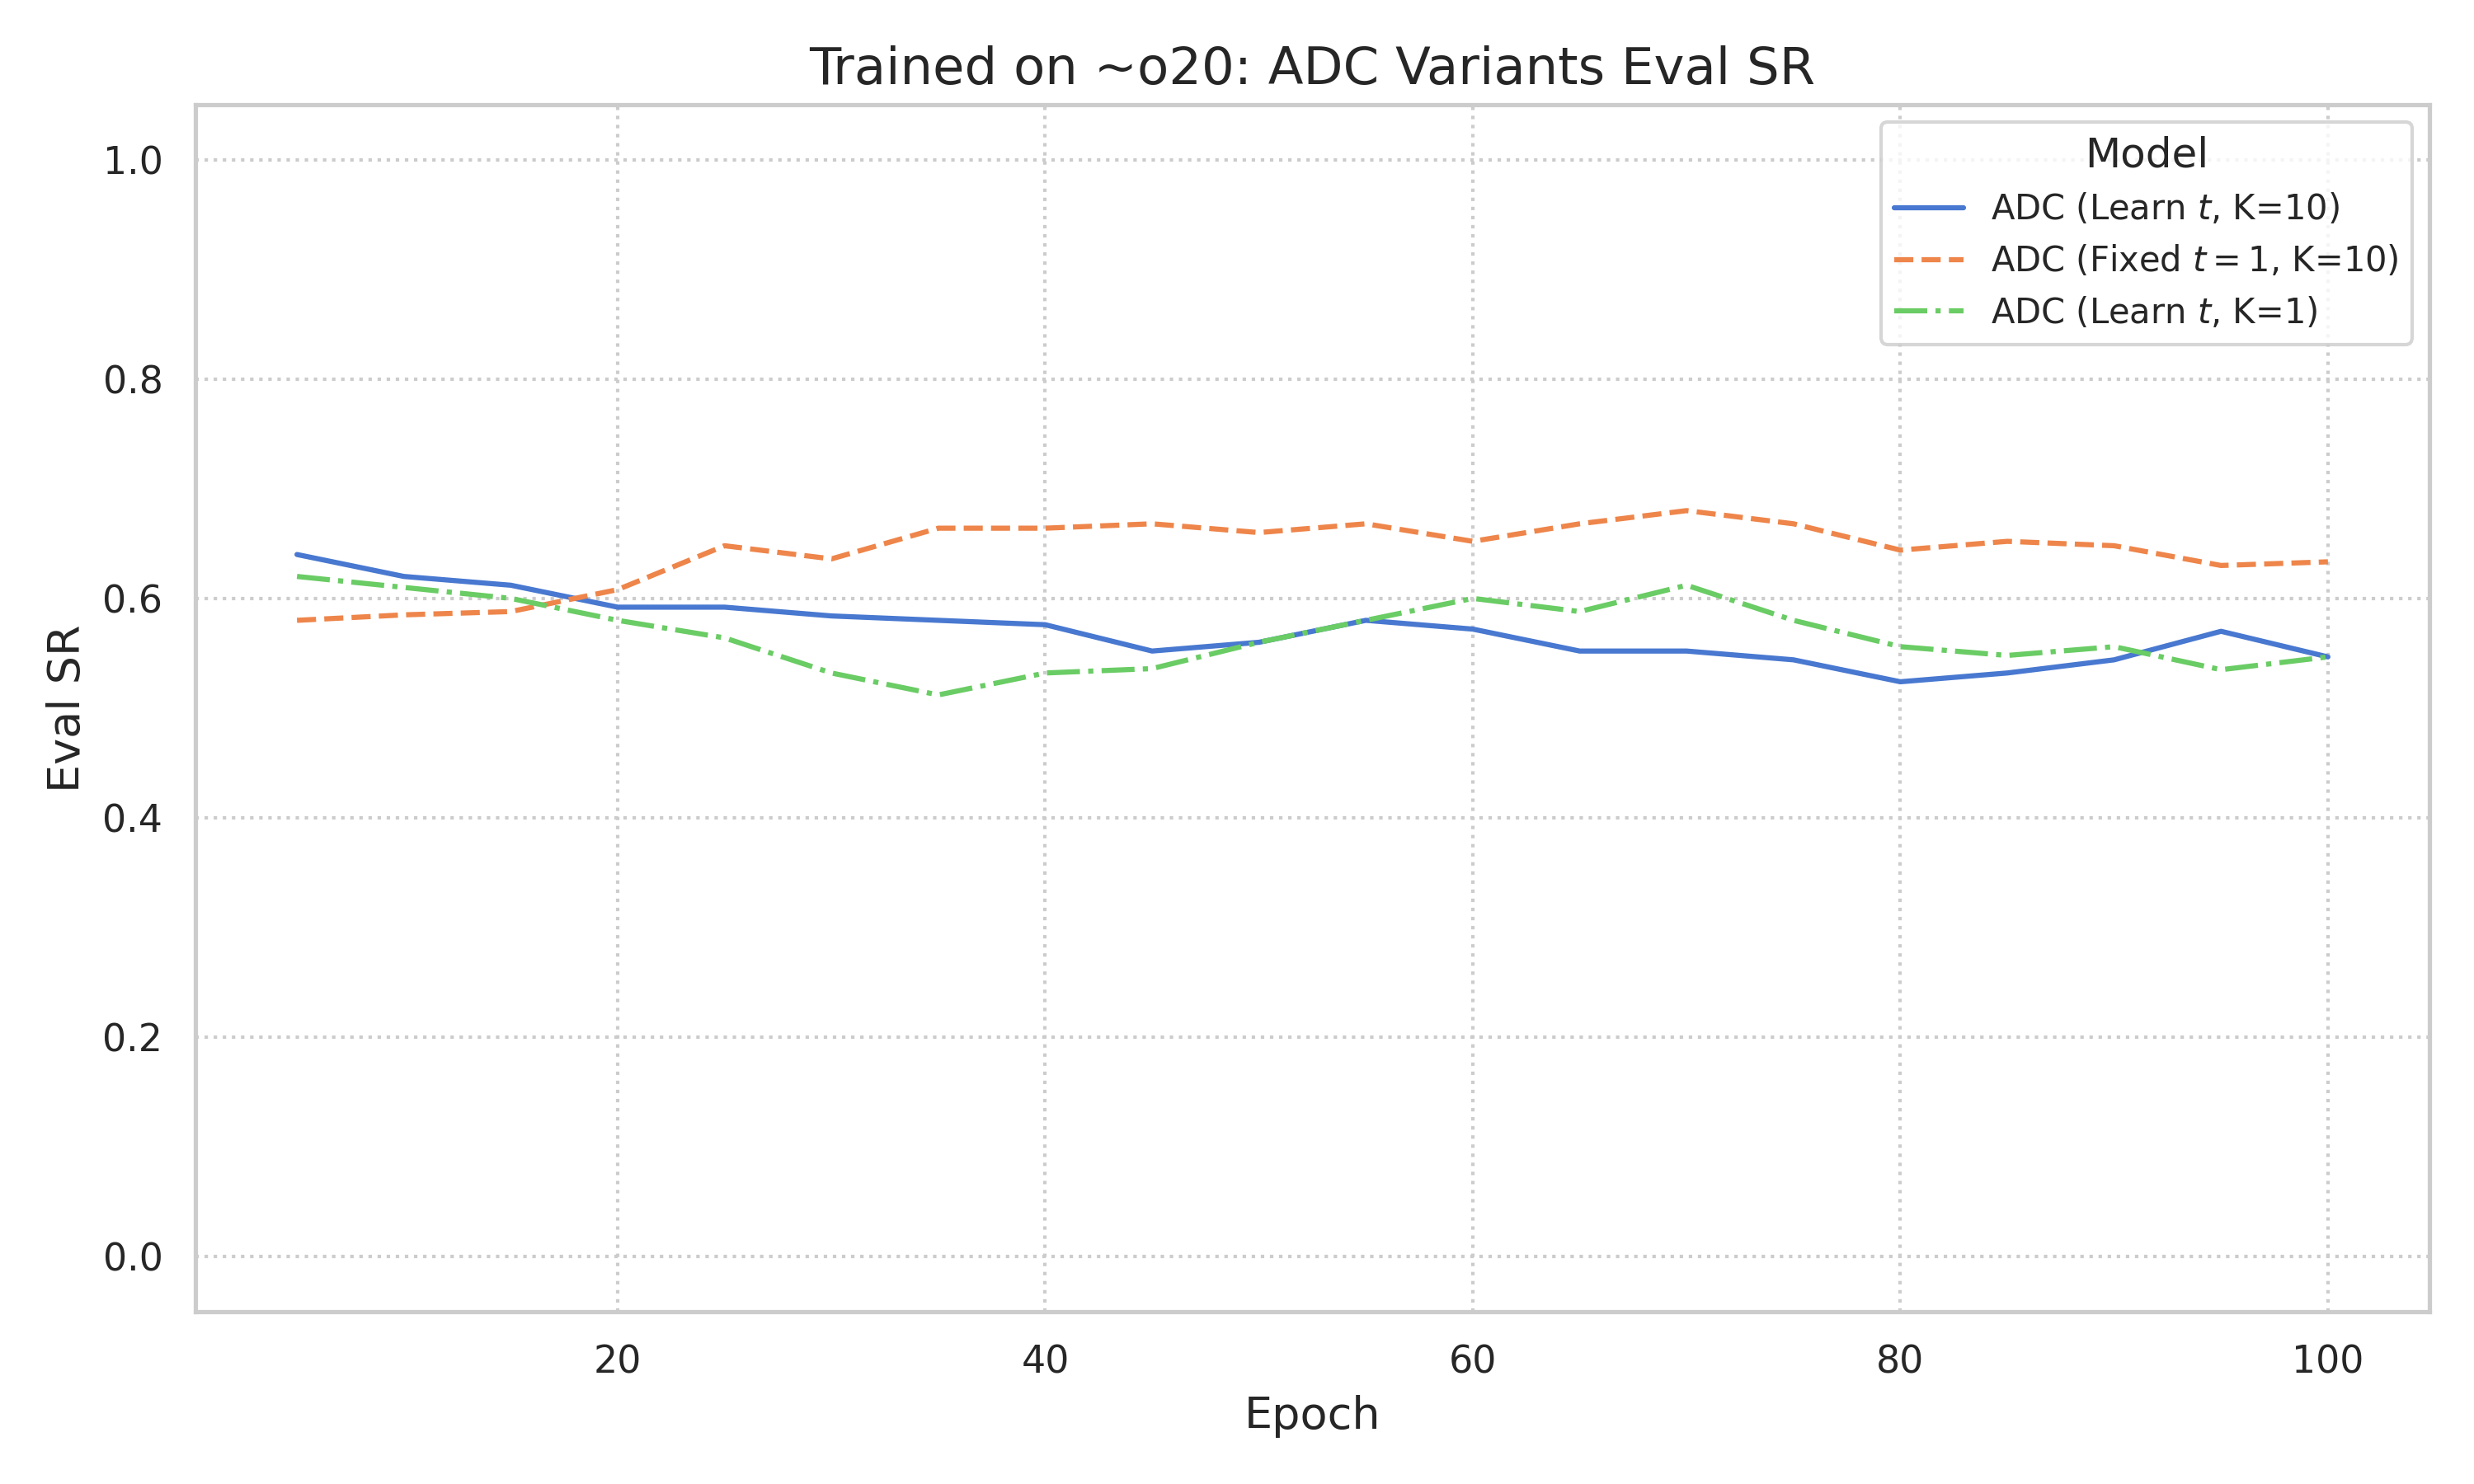
\includegraphics[width=\textwidth]{trainplotbase/TRAINED_ON_20_OBS/training_curves_focused/condition_o20/adc_variants_eval_sr.png} % UPDATE PATH
        \caption{ADC Variants: Validation SR (20\% Obst.)}
        \label{fig:adc_val_sr_20obs}
    \end{subfigure}

    \vspace{0.3cm}

    % Row 2
    \begin{subfigure}[b]{0.48\textwidth}
        \centering
        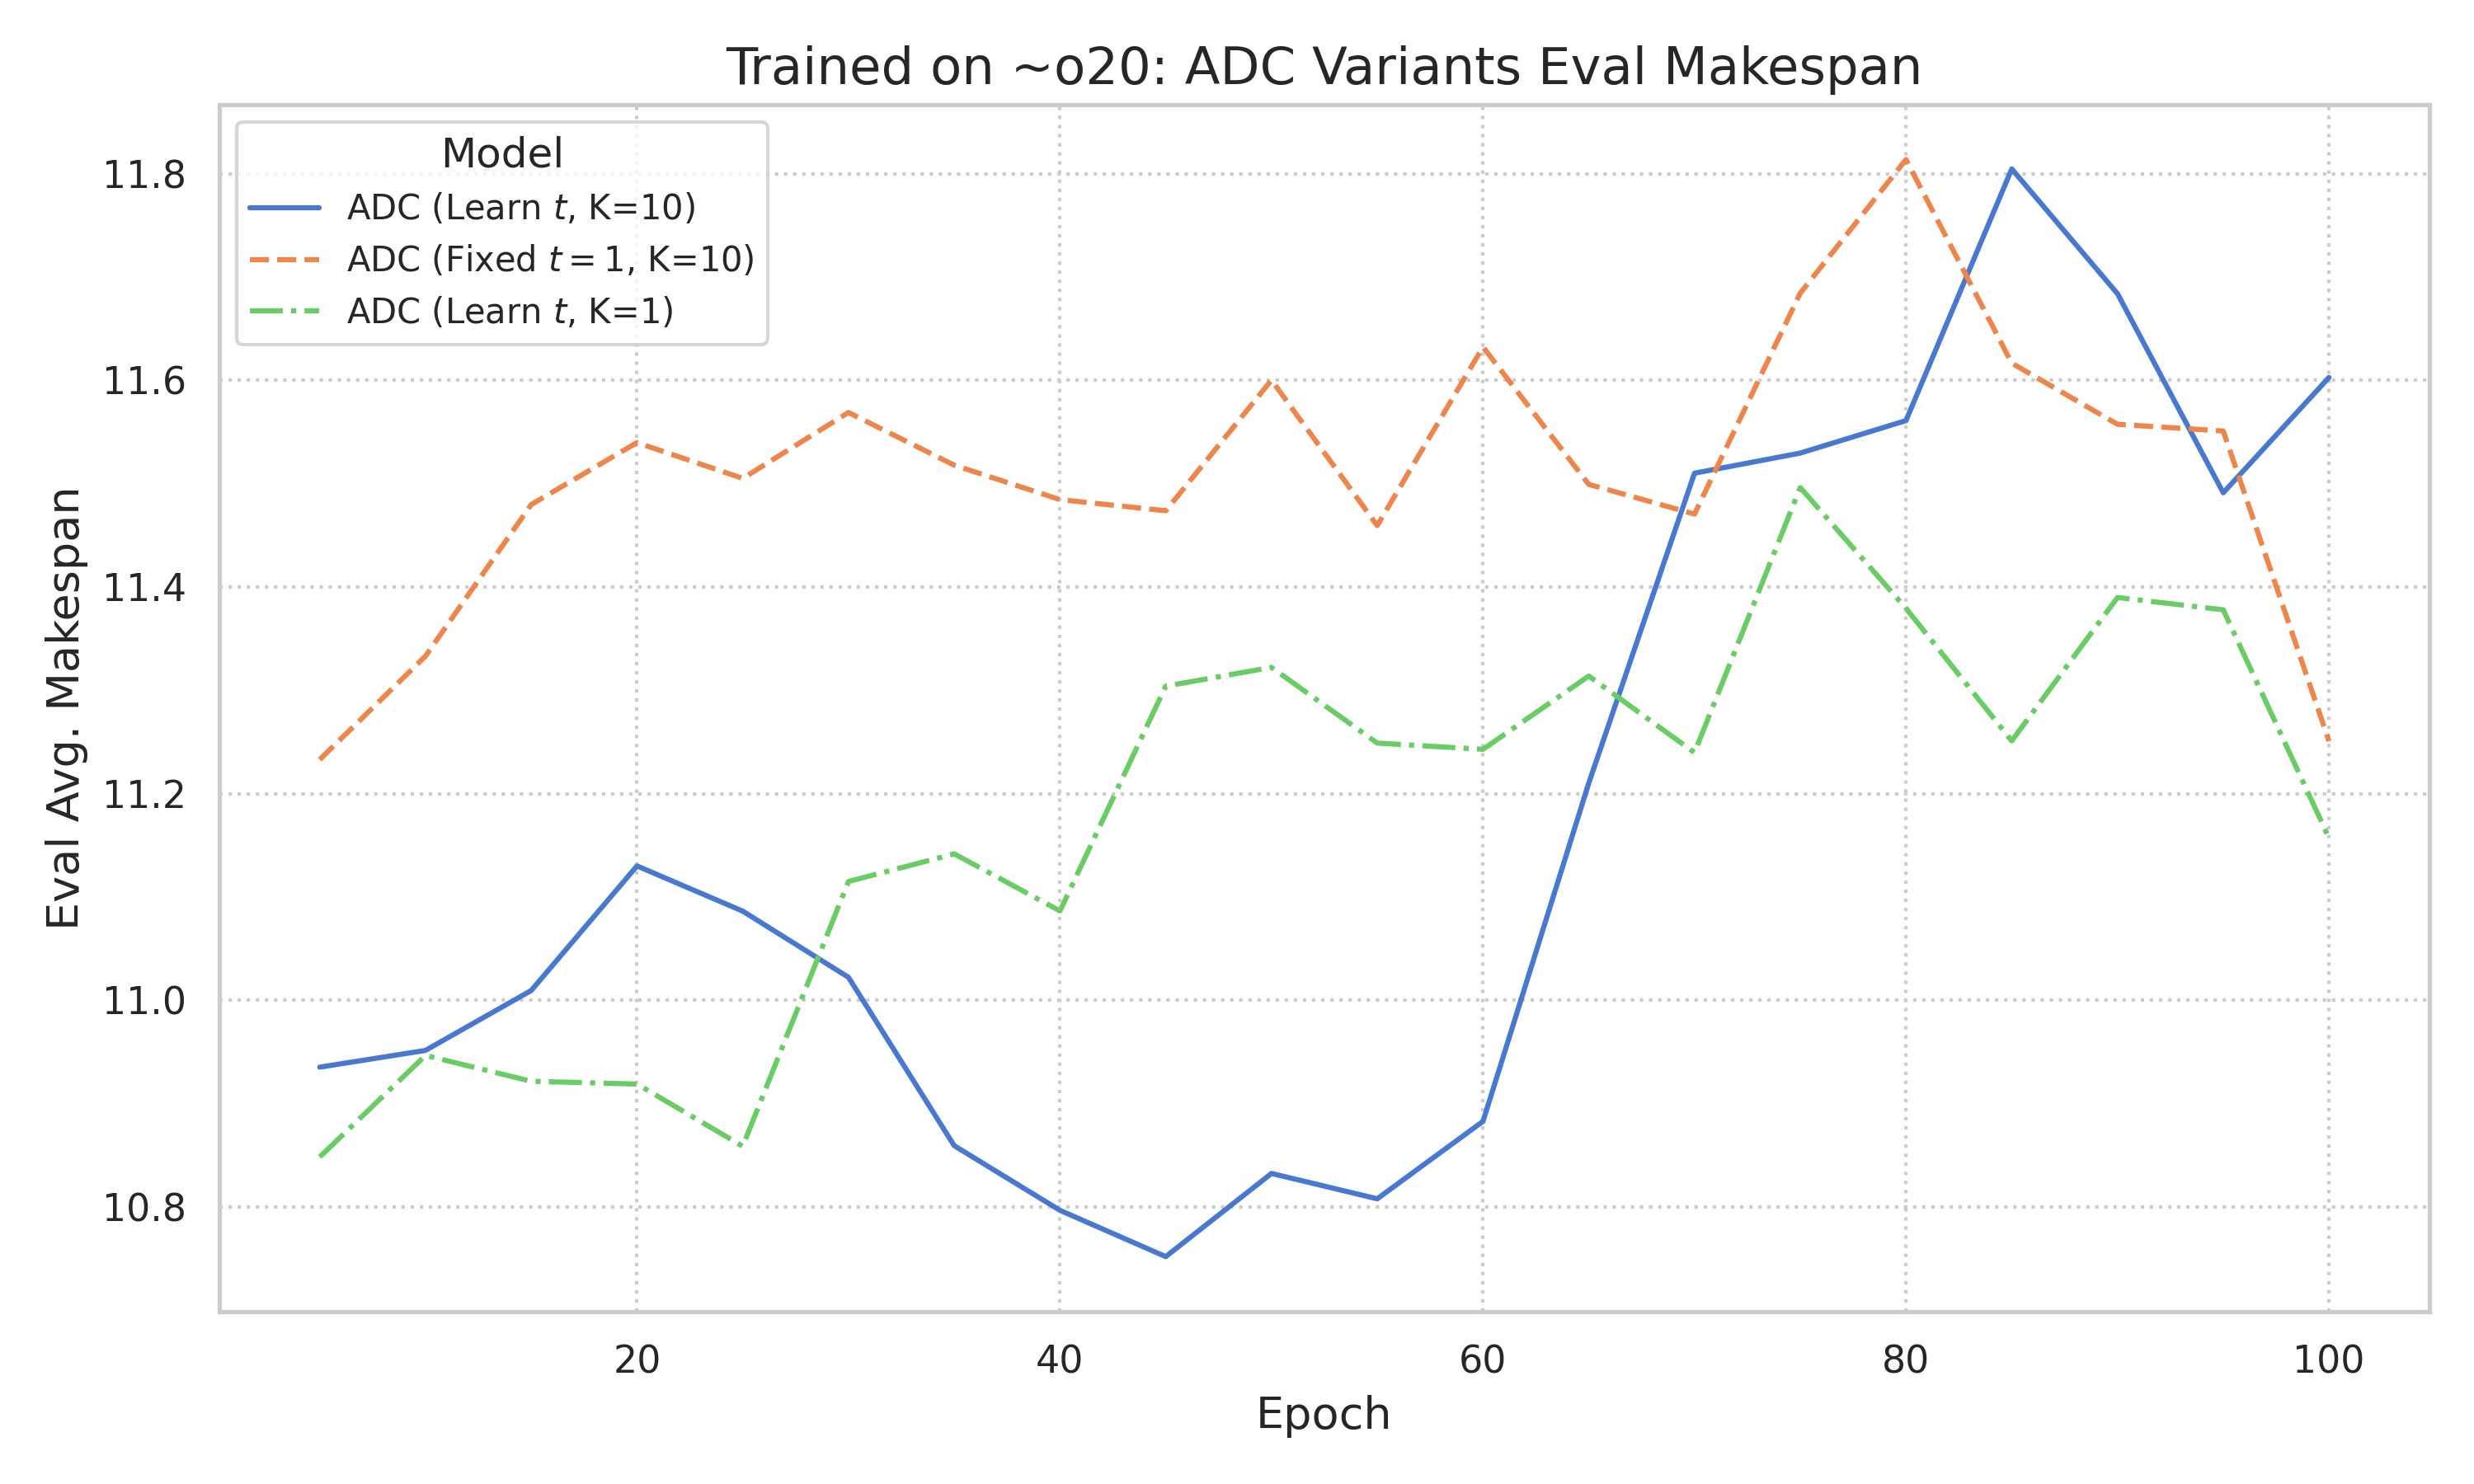
\includegraphics[width=\textwidth]{trainplotbase/TRAINED_ON_20_OBS/training_curves_focused/condition_o20/adc_variants_eval_am.png} % UPDATE PATH
        \caption{ADC Variants: Validation AM (20\% Obst.)}
        \label{fig:adc_val_am_20obs}
    \end{subfigure}
    \hfill
    \begin{subfigure}[b]{0.48\textwidth}
        \centering
        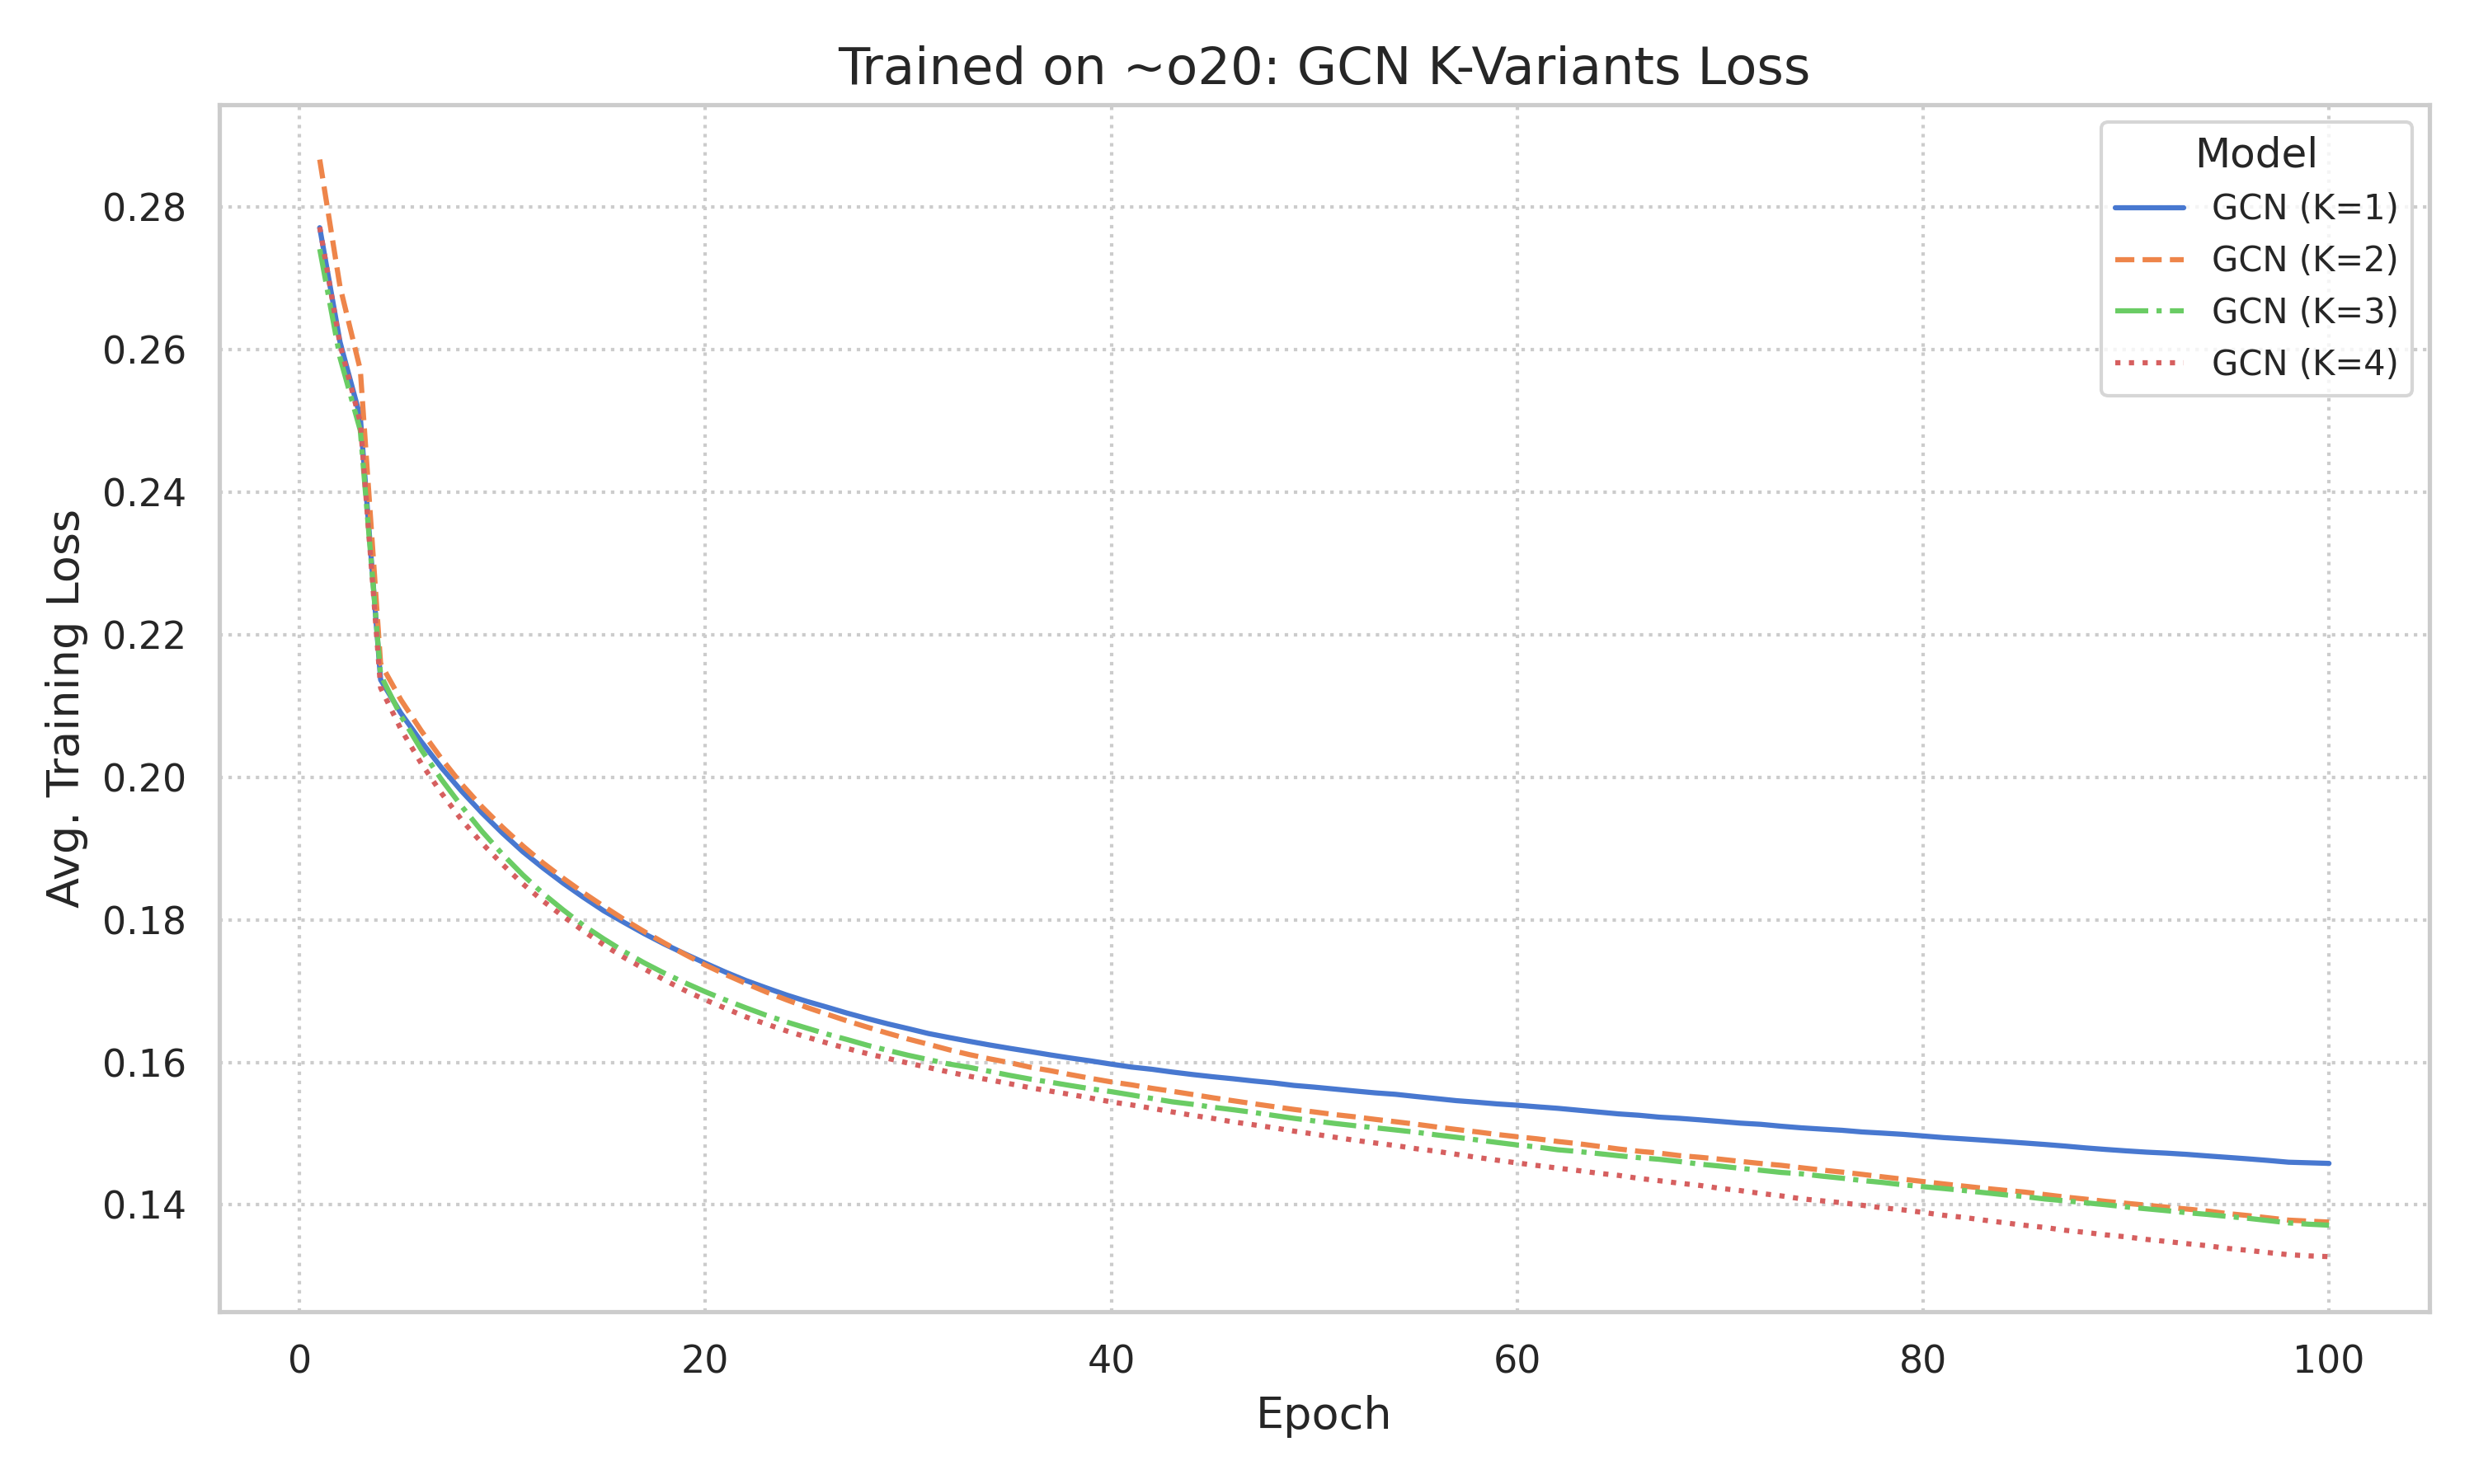
\includegraphics[width=\textwidth]{trainplotbase/TRAINED_ON_20_OBS/training_curves_focused/condition_o20/gcn_variants_train_loss.png} % UPDATE PATH
        \caption{GCN Variants: Training Loss (20\% Obst.)}
        \label{fig:gcn_train_loss_20obs}
    \end{subfigure}

    \vspace{0.3cm}

    % Row 3
    \begin{subfigure}[b]{0.48\textwidth}
        \centering
        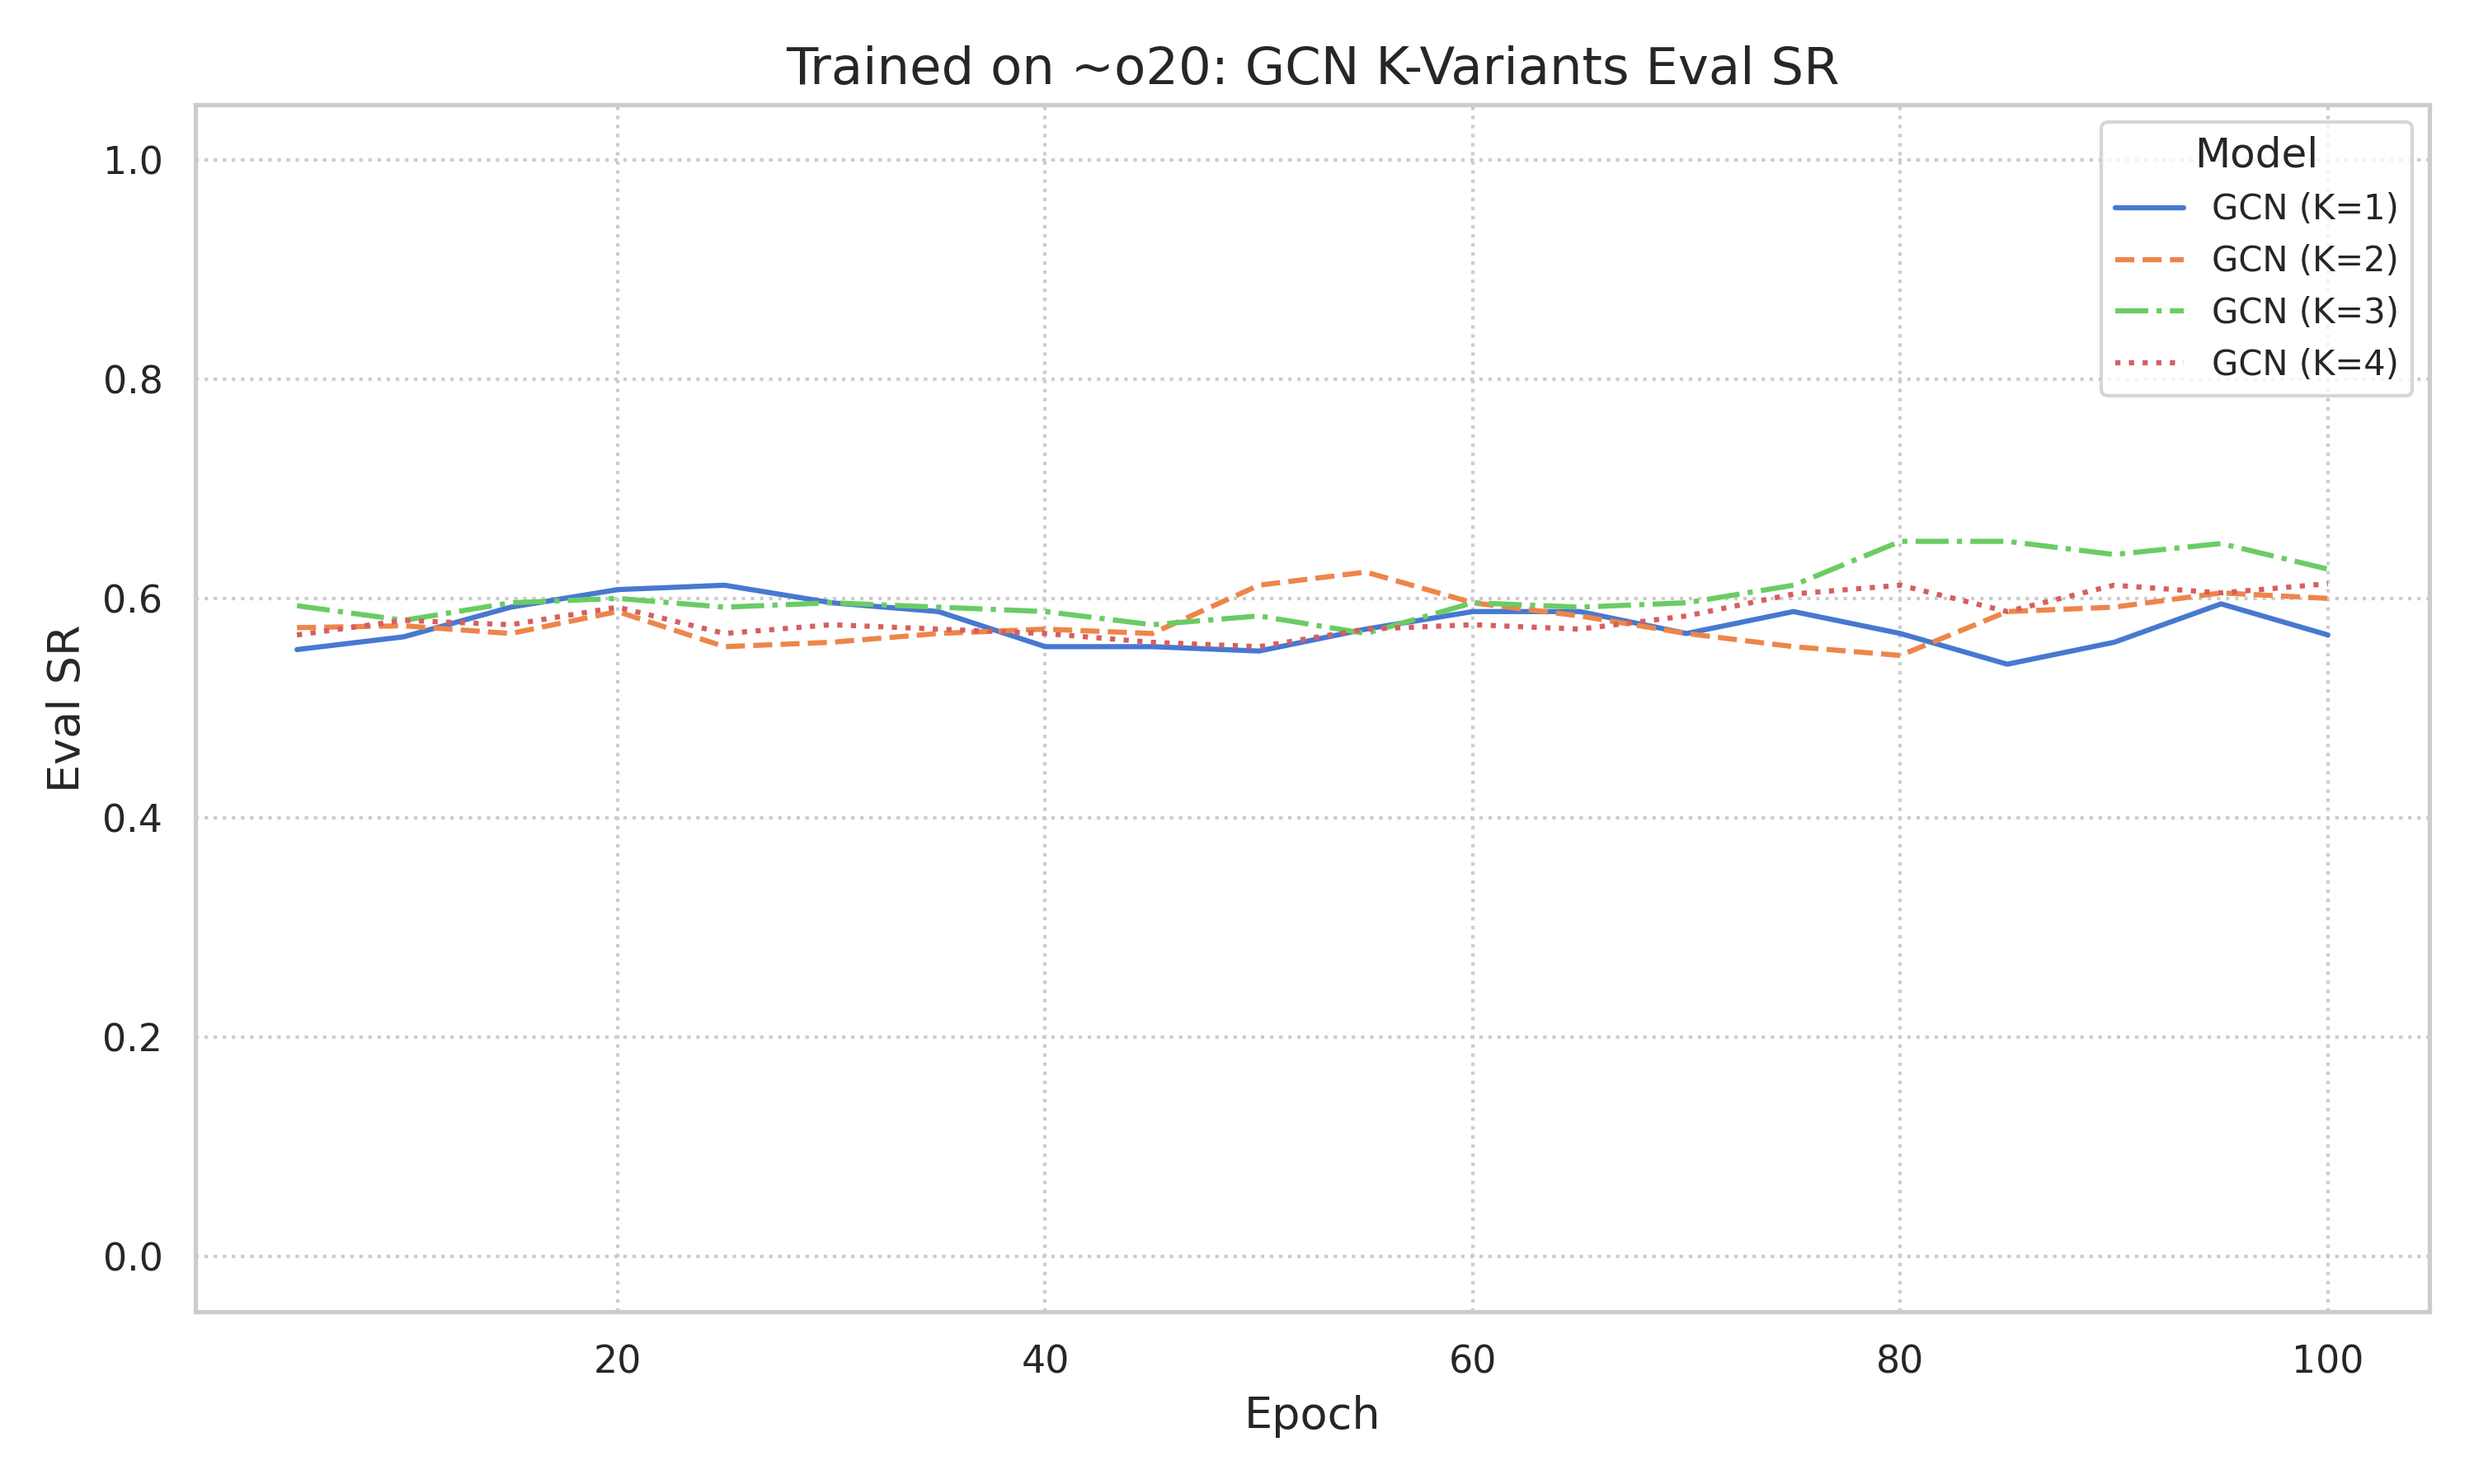
\includegraphics[width=\textwidth]{trainplotbase/TRAINED_ON_20_OBS/training_curves_focused/condition_o20/gcn_variants_eval_sr.png} % UPDATE PATH
        \caption{GCN Variants: Validation SR (20\% Obst.)}
        \label{fig:gcn_val_sr_20obs}
    \end{subfigure}
    \hfill
    \begin{subfigure}[b]{0.48\textwidth}
        \centering
        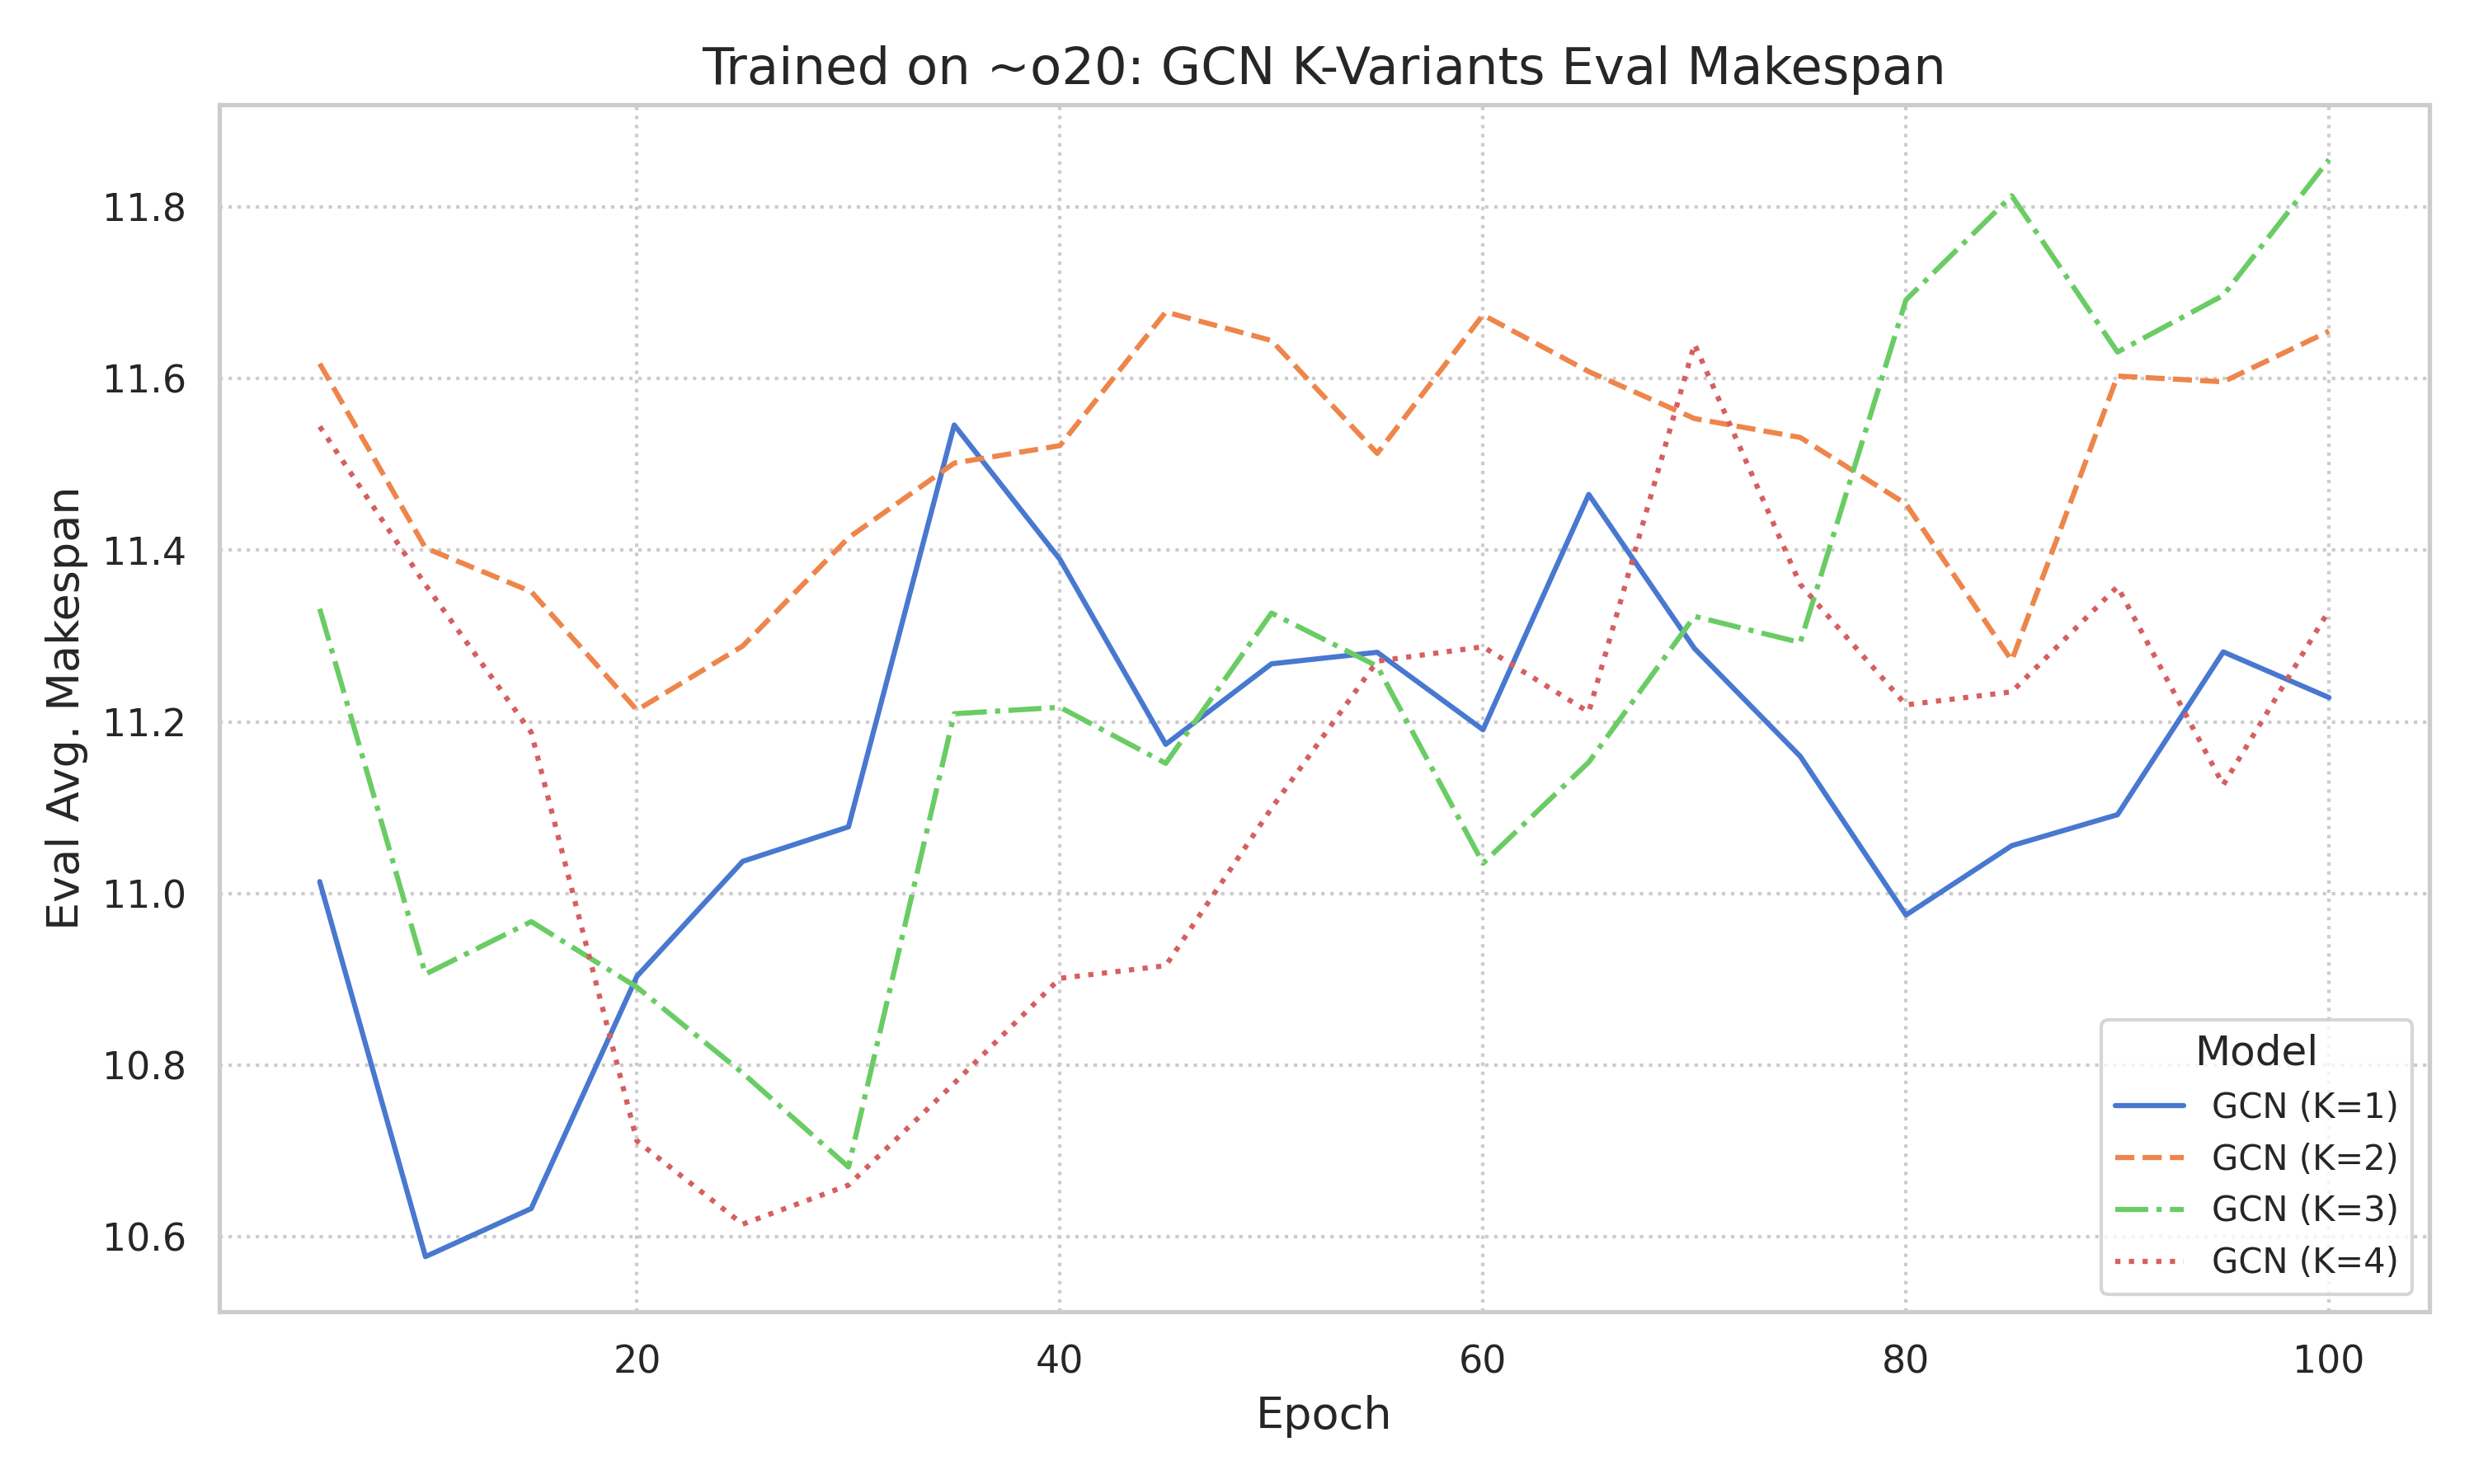
\includegraphics[width=\textwidth]{trainplotbase/TRAINED_ON_20_OBS/training_curves_focused/condition_o20/gcn_variants_eval_am.png} % UPDATE PATH
        \caption{GCN Variants: Validation AM (20\% Obst.)}
        \label{fig:gcn_val_am_20obs}
    \end{subfigure}

    \caption{Training progress for models trained on the 20\% obstacle density dataset. Layout and metrics are consistent with Figure~\ref{fig:training_curves_10obs_improved}.}
    \label{fig:training_curves_20obs_improved}
\end{figure}


\subsection{Training on 30\% Obstacle Density Dataset}
\label{subsec:training_30obs}
Finally, models were trained on the most challenging dataset with 30\% obstacle density. Figure~\ref{fig:training_curves_30obs_improved} shows the training progression for these models.

\begin{figure}[htbp]
    \centering
    % ADC Variants - Trained on 30% Obstacles
    \begin{subfigure}[b]{0.48\textwidth}
        \centering
        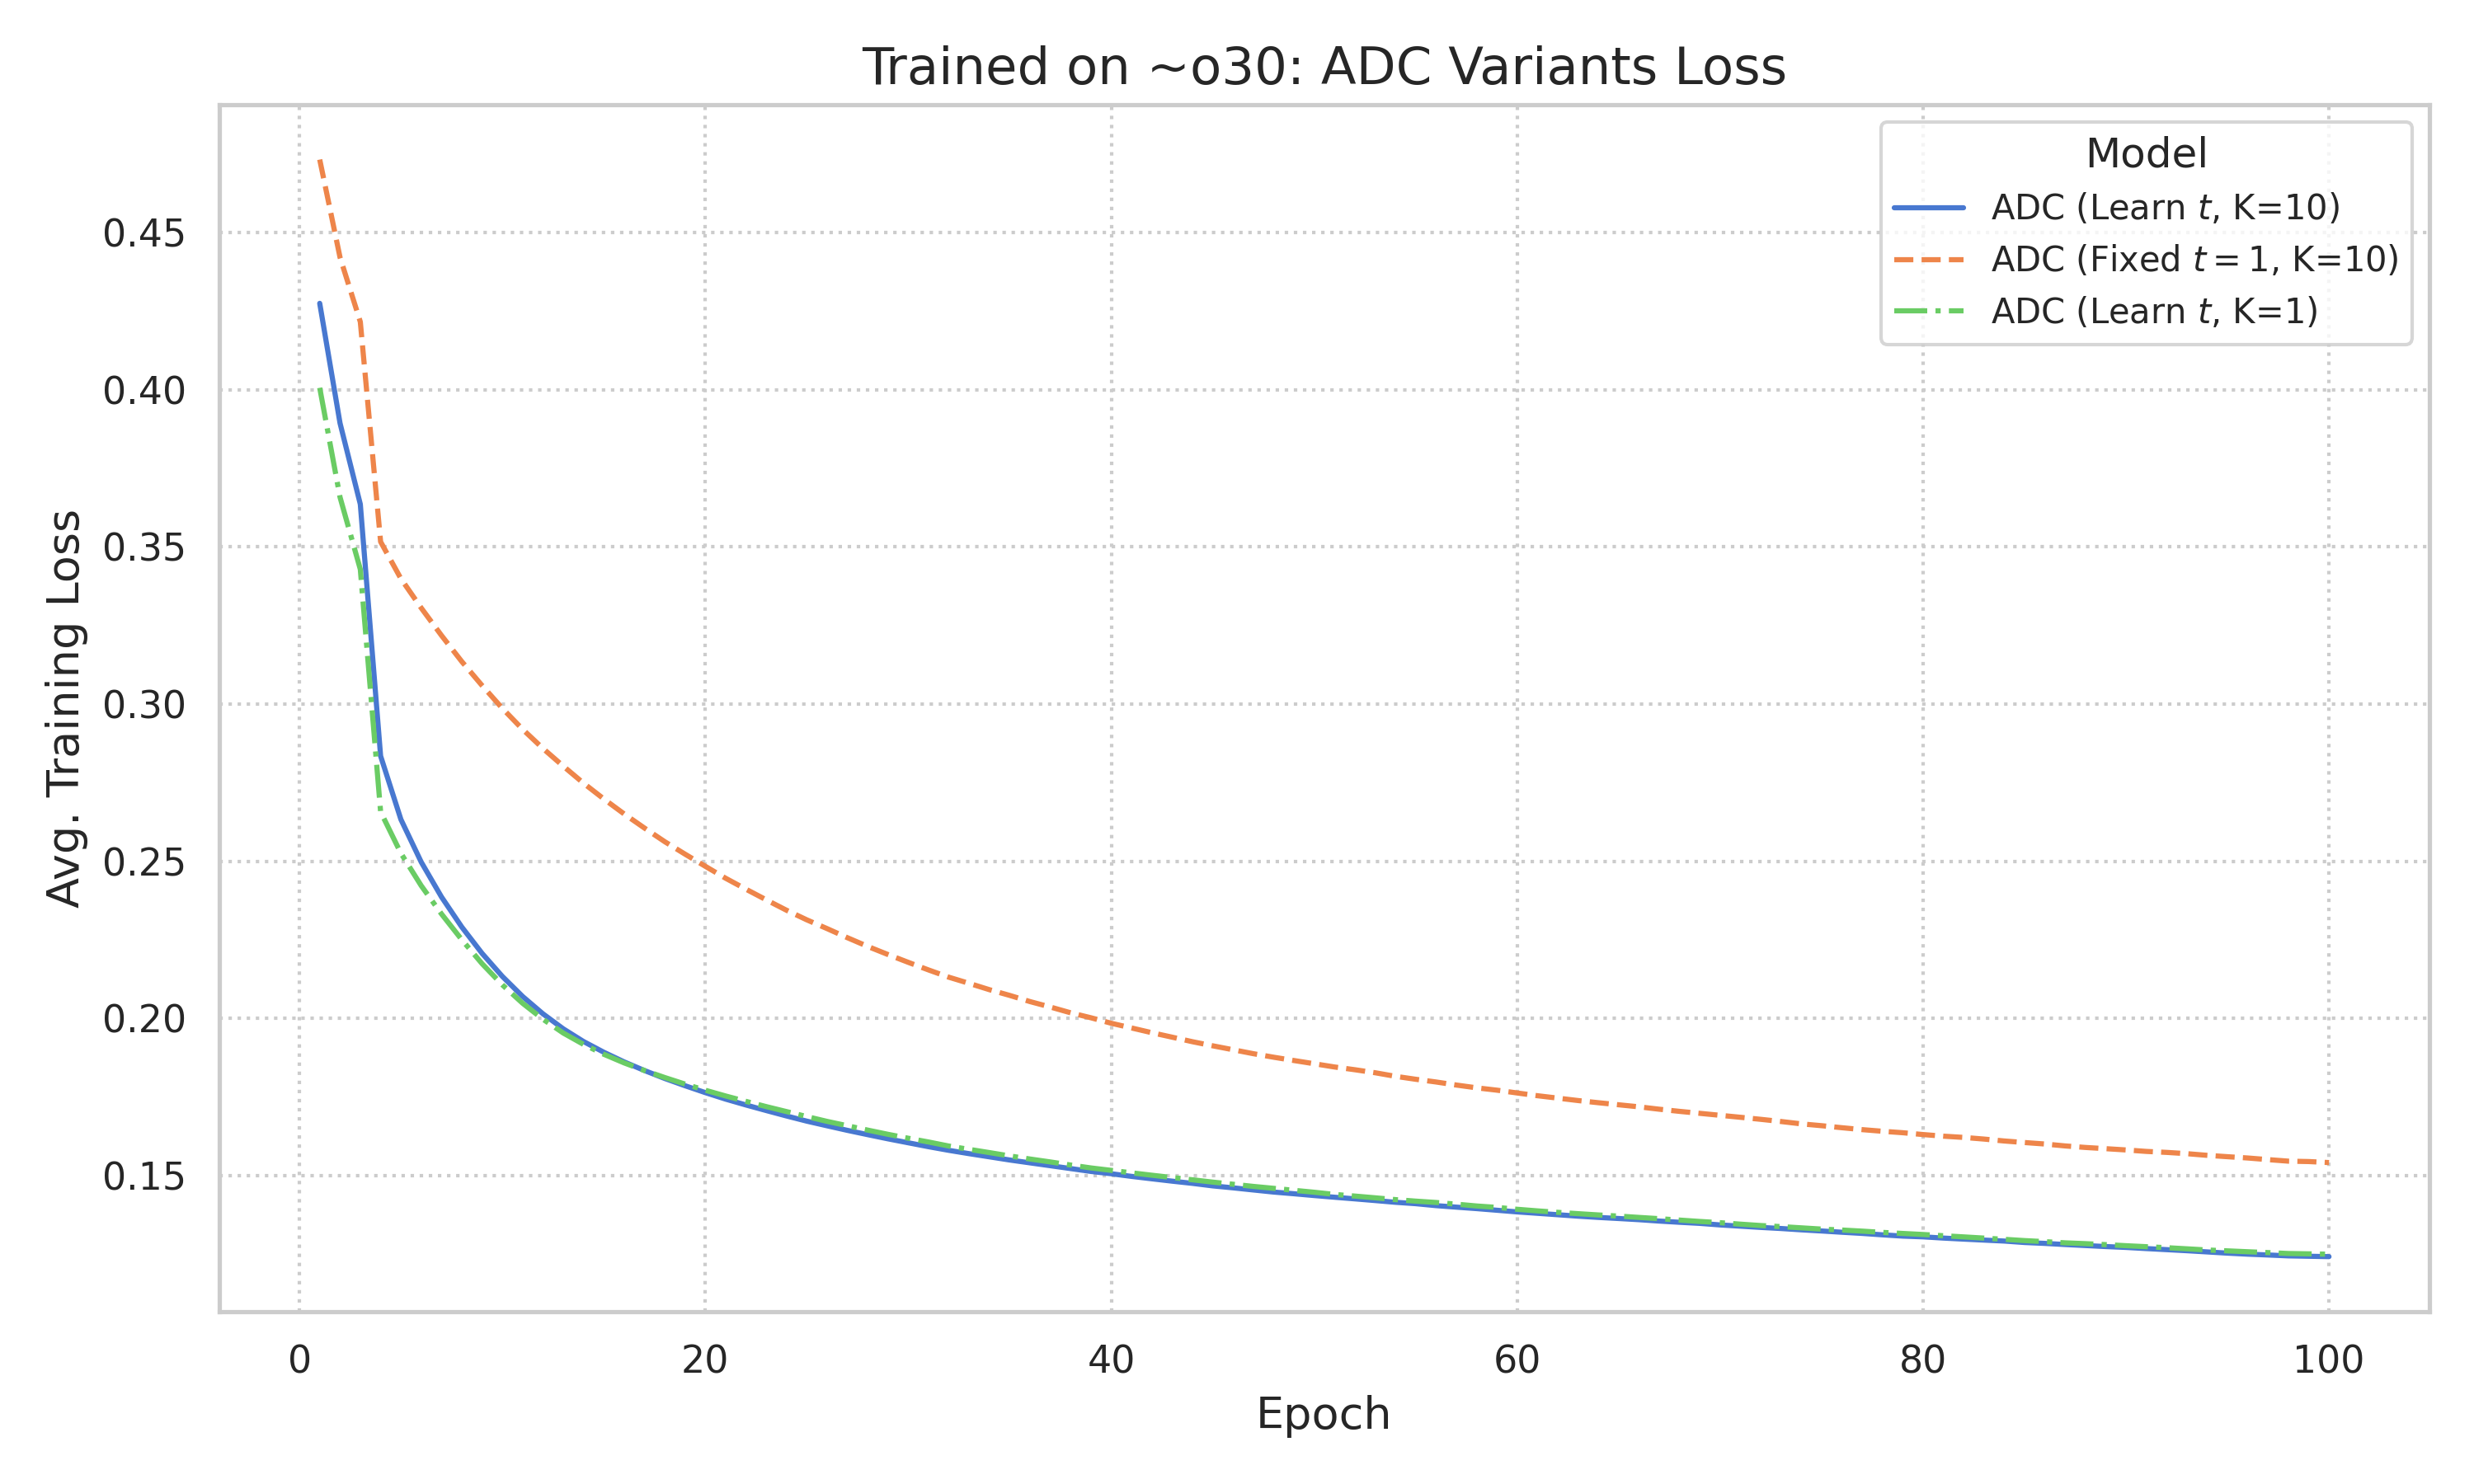
\includegraphics[width=\textwidth]{trainplotbase/TRAINED_ON_30_OBS/training_curves_focused/condition_o30/adc_variants_train_loss.png} % UPDATE PATH
        \caption{ADC Variants: Training Loss (30\% Obst.)}
        \label{fig:adc_train_loss_30obs}
    \end{subfigure}
    \hfill
    \begin{subfigure}[b]{0.48\textwidth}
        \centering
        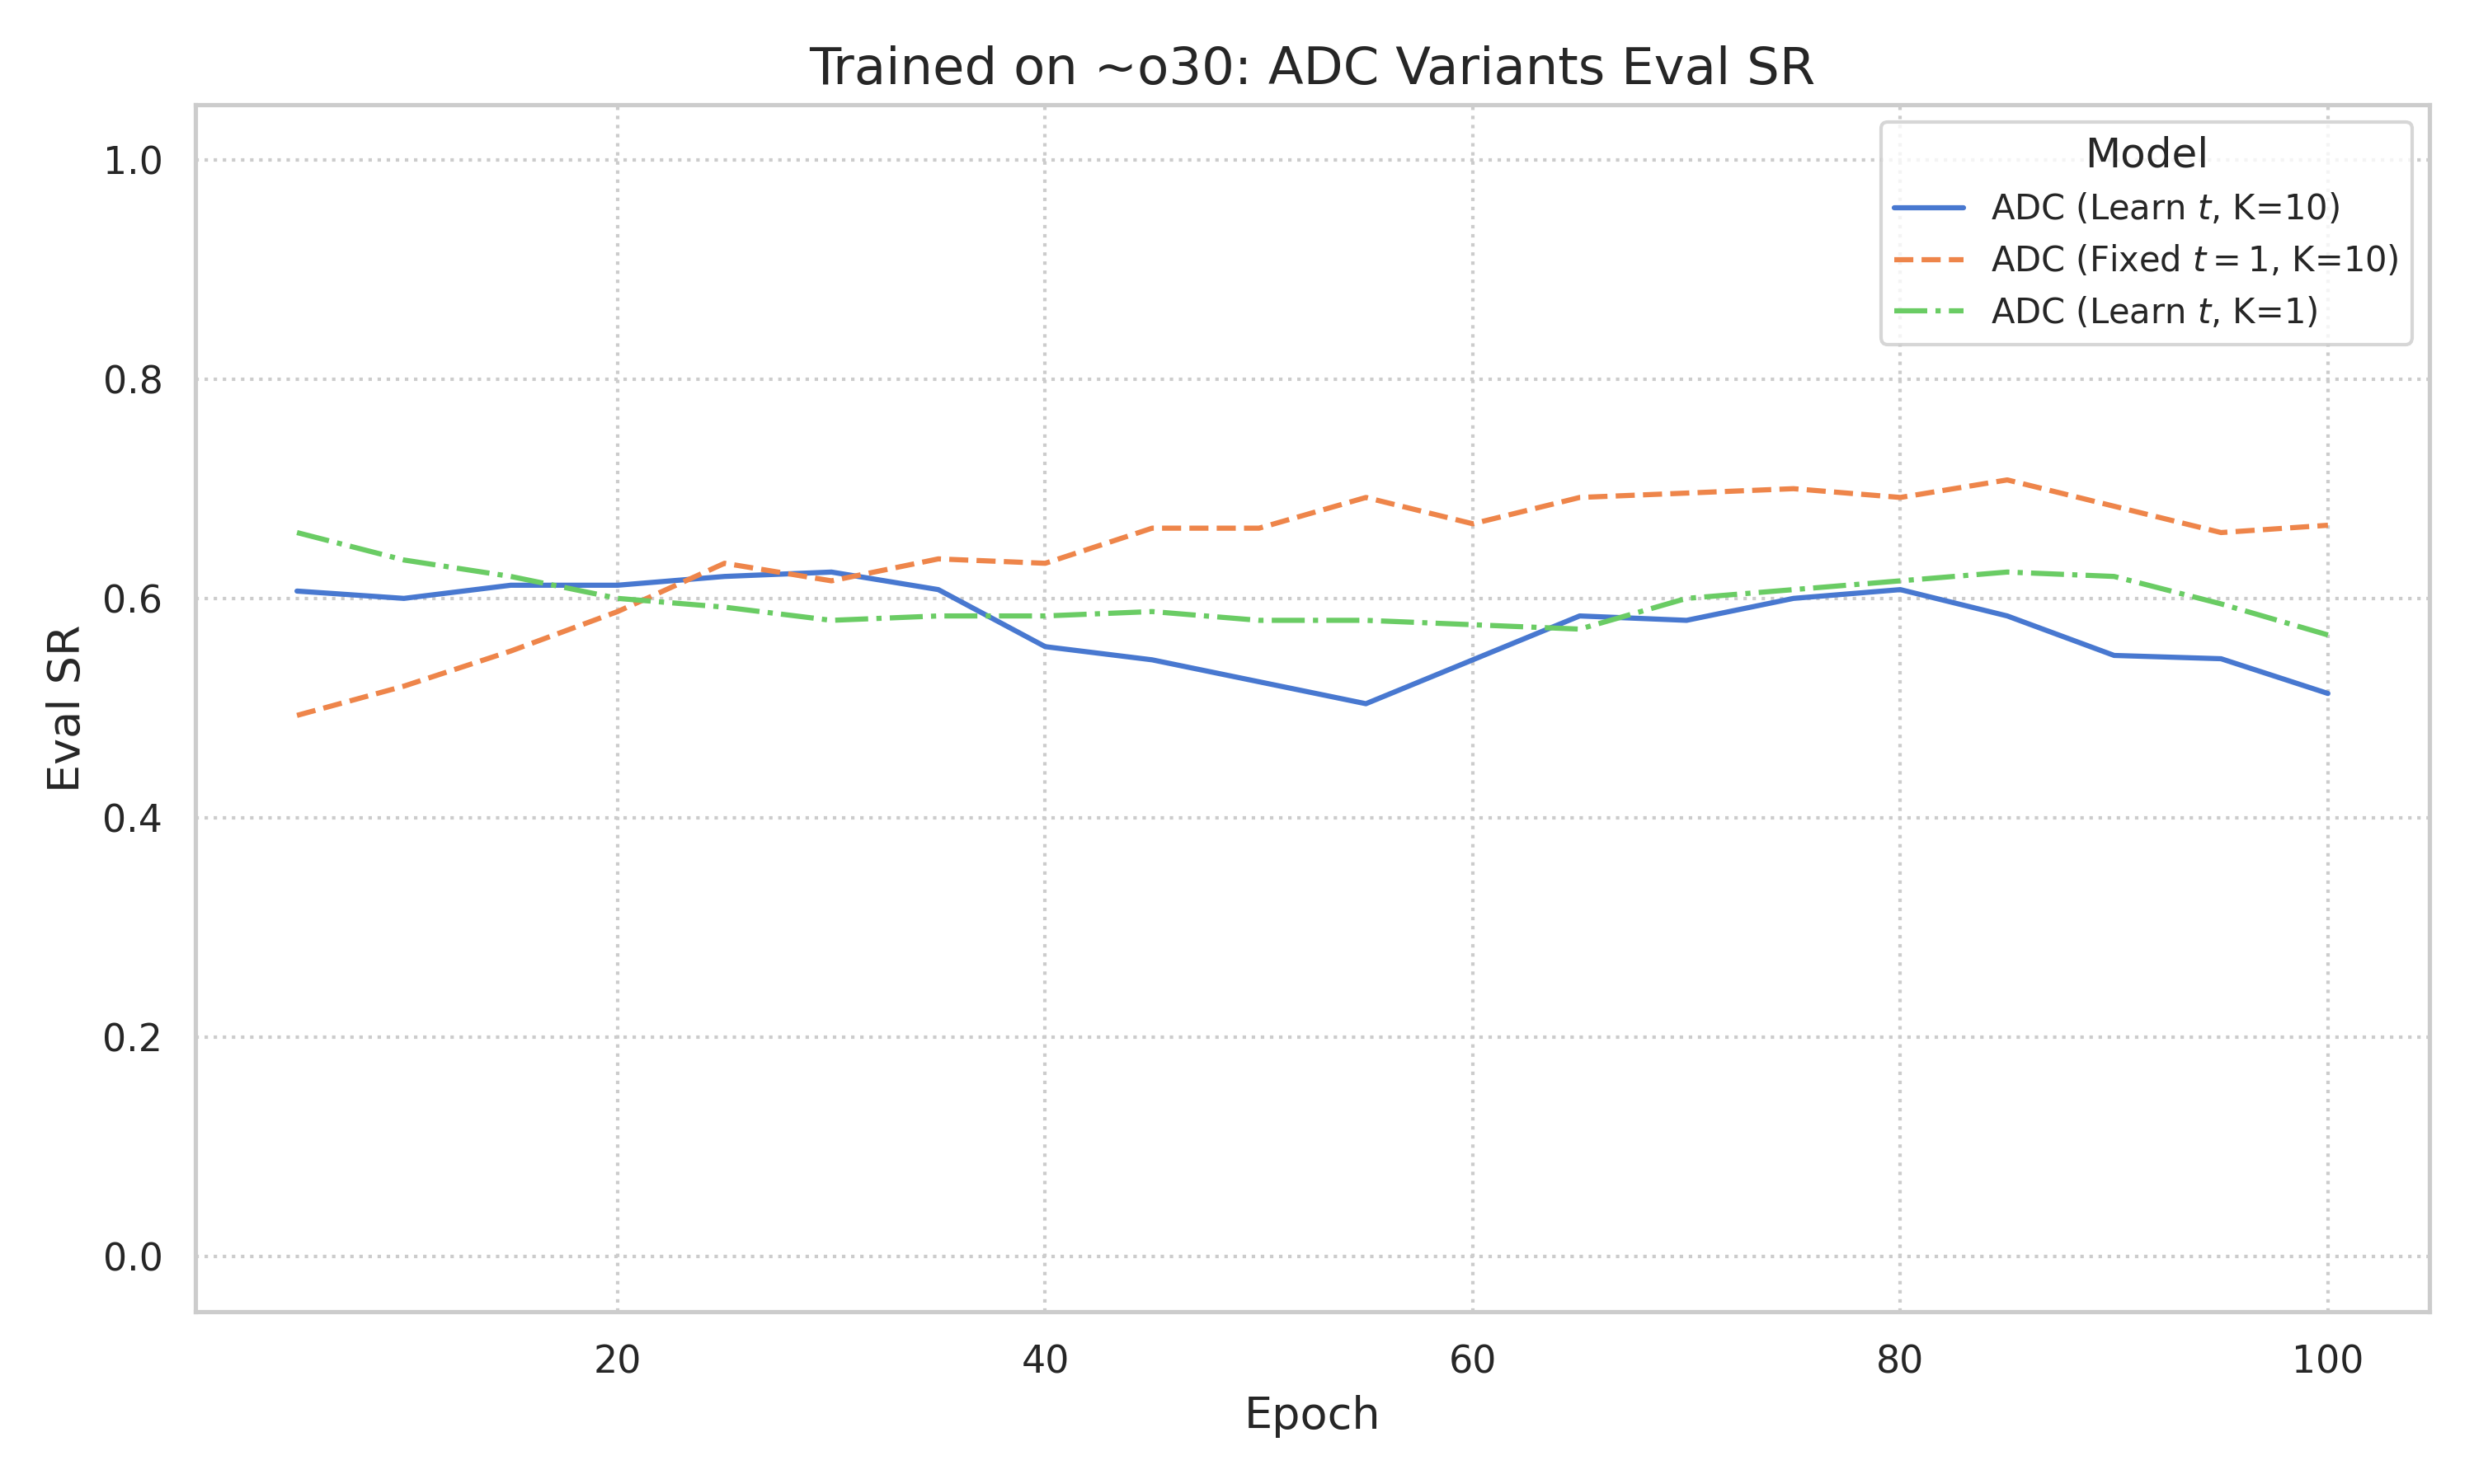
\includegraphics[width=\textwidth]{trainplotbase/TRAINED_ON_30_OBS/training_curves_focused/condition_o30/adc_variants_eval_sr.png} % UPDATE PATH
        \caption{ADC Variants: Validation SR (30\% Obst.)}
        \label{fig:adc_val_sr_30obs}
    \end{subfigure}

    \vspace{0.3cm}

    % Row 2
    \begin{subfigure}[b]{0.48\textwidth}
        \centering
        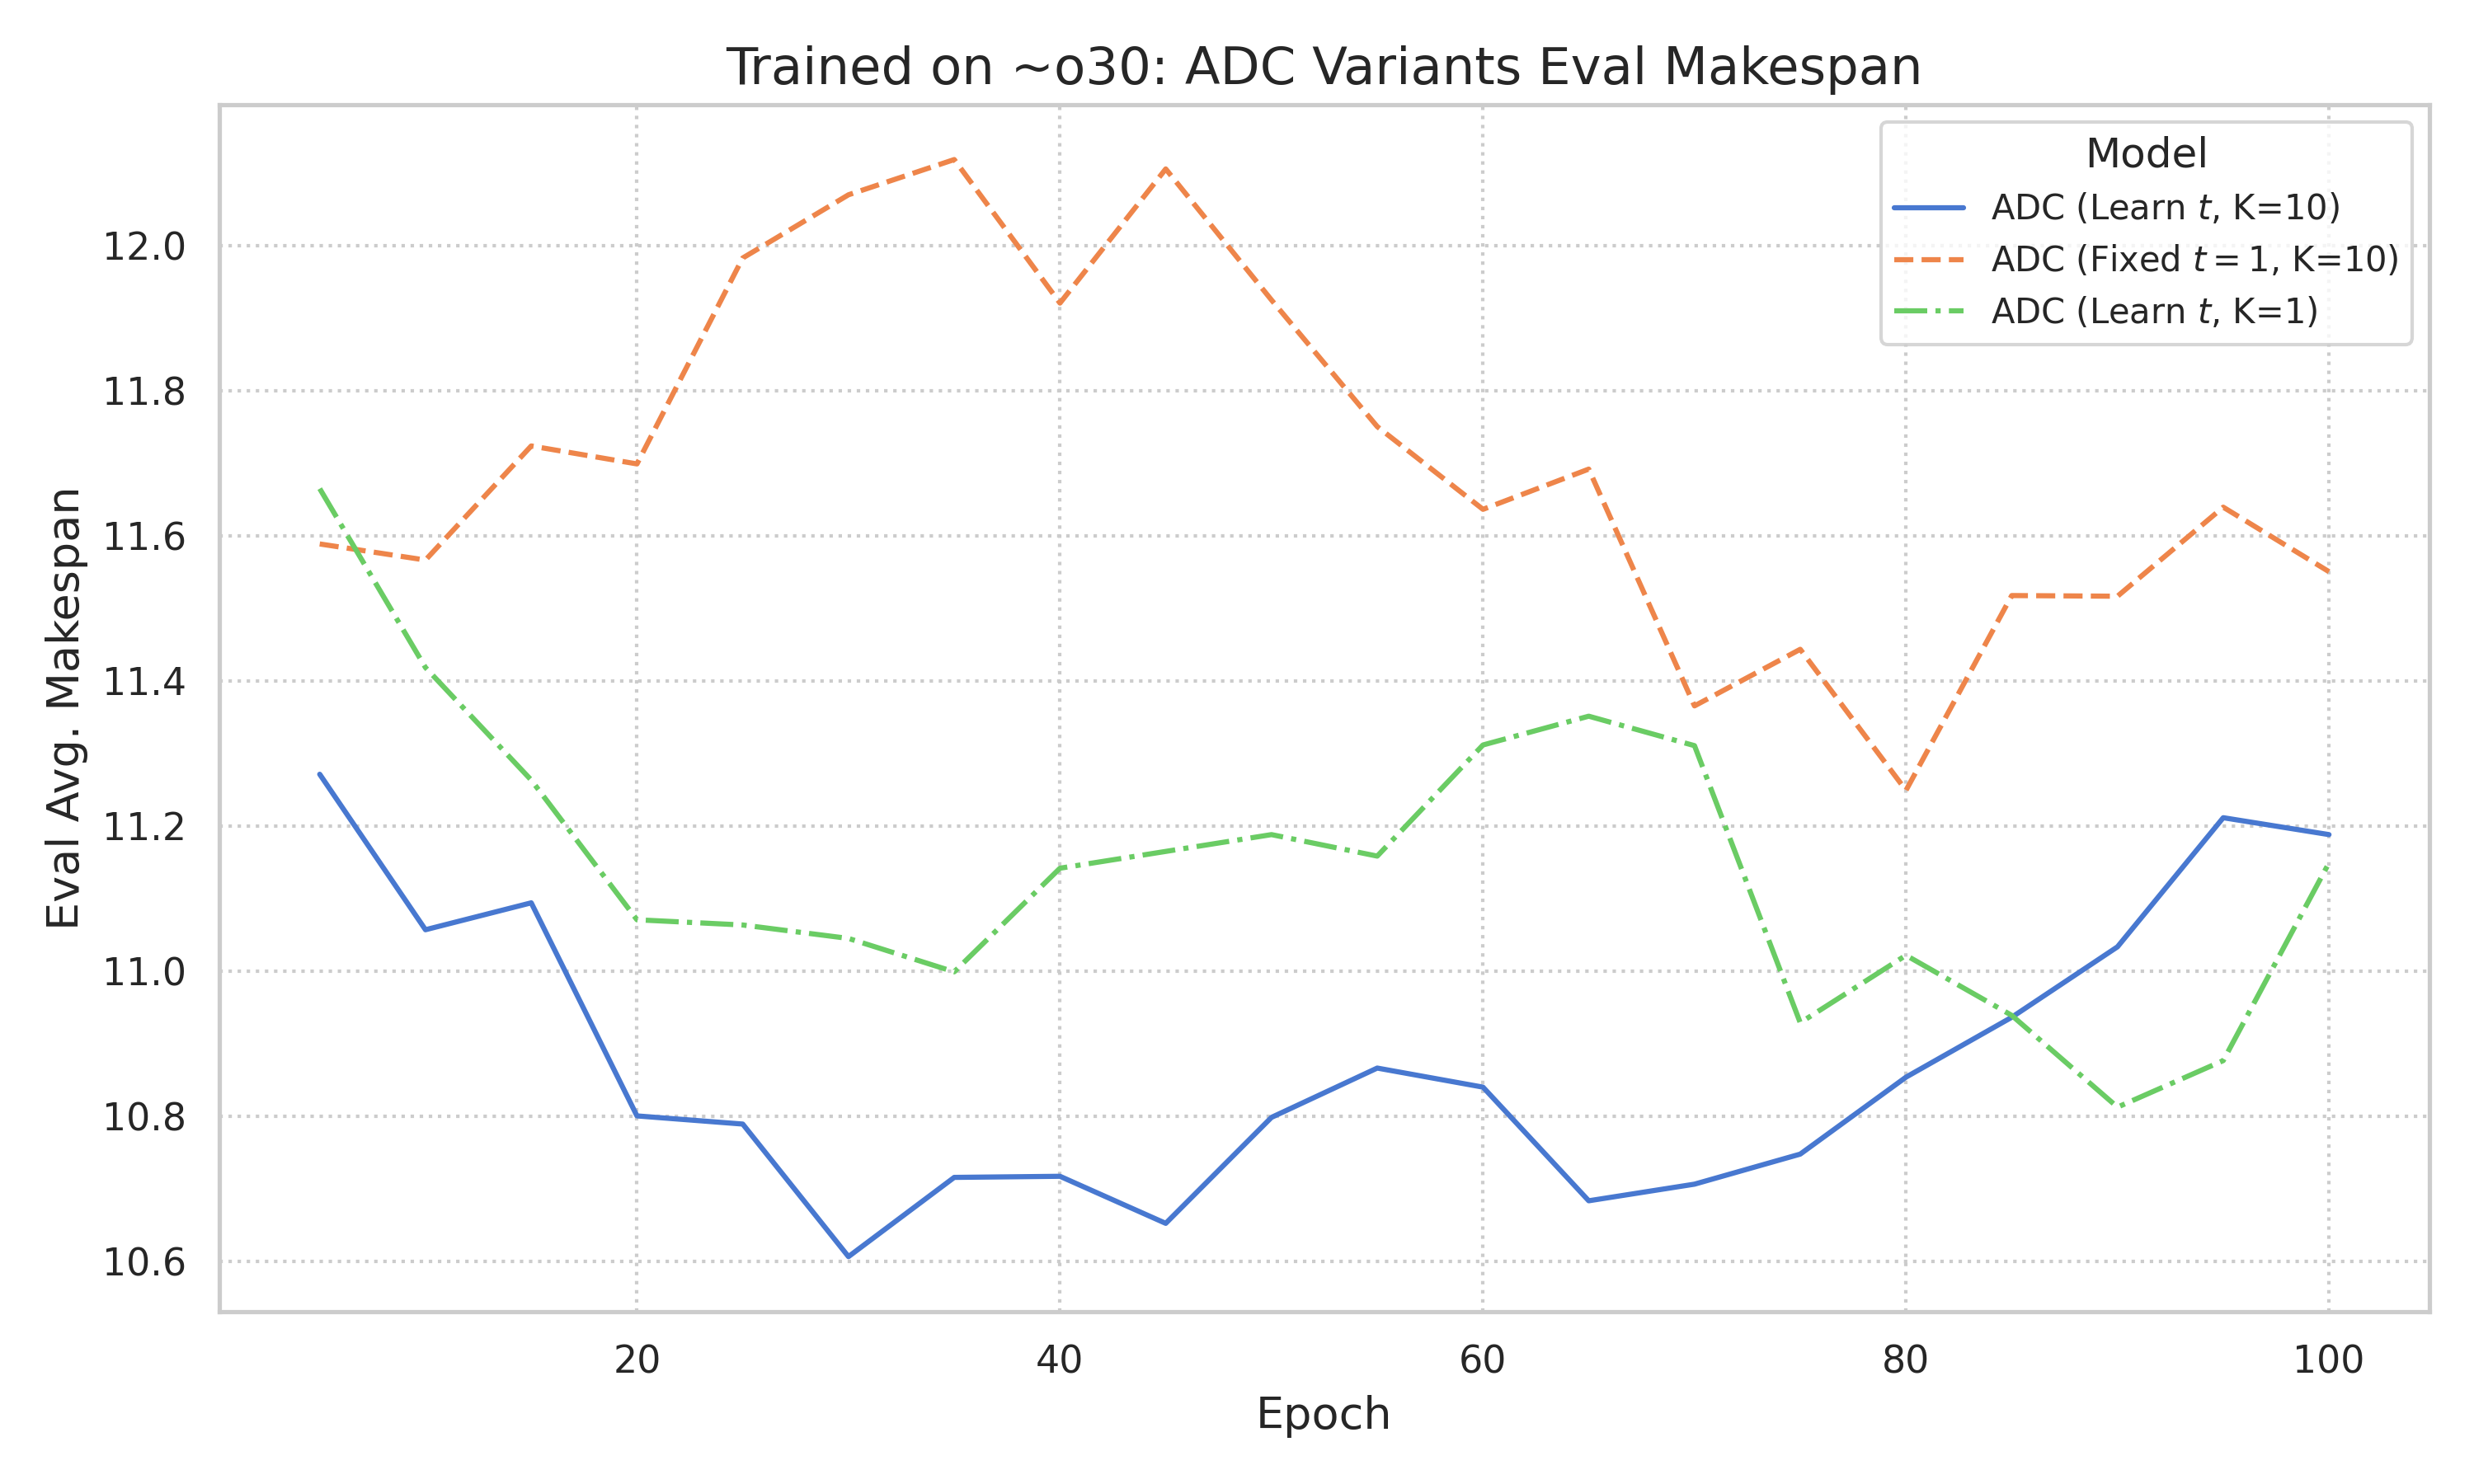
\includegraphics[width=\textwidth]{trainplotbase/TRAINED_ON_30_OBS/training_curves_focused/condition_o30/adc_variants_eval_am.png} % UPDATE PATH
        \caption{ADC Variants: Validation AM (30\% Obst.)}
        \label{fig:adc_val_am_30obs}
    \end{subfigure}
    \hfill
    \begin{subfigure}[b]{0.48\textwidth}
        \centering
        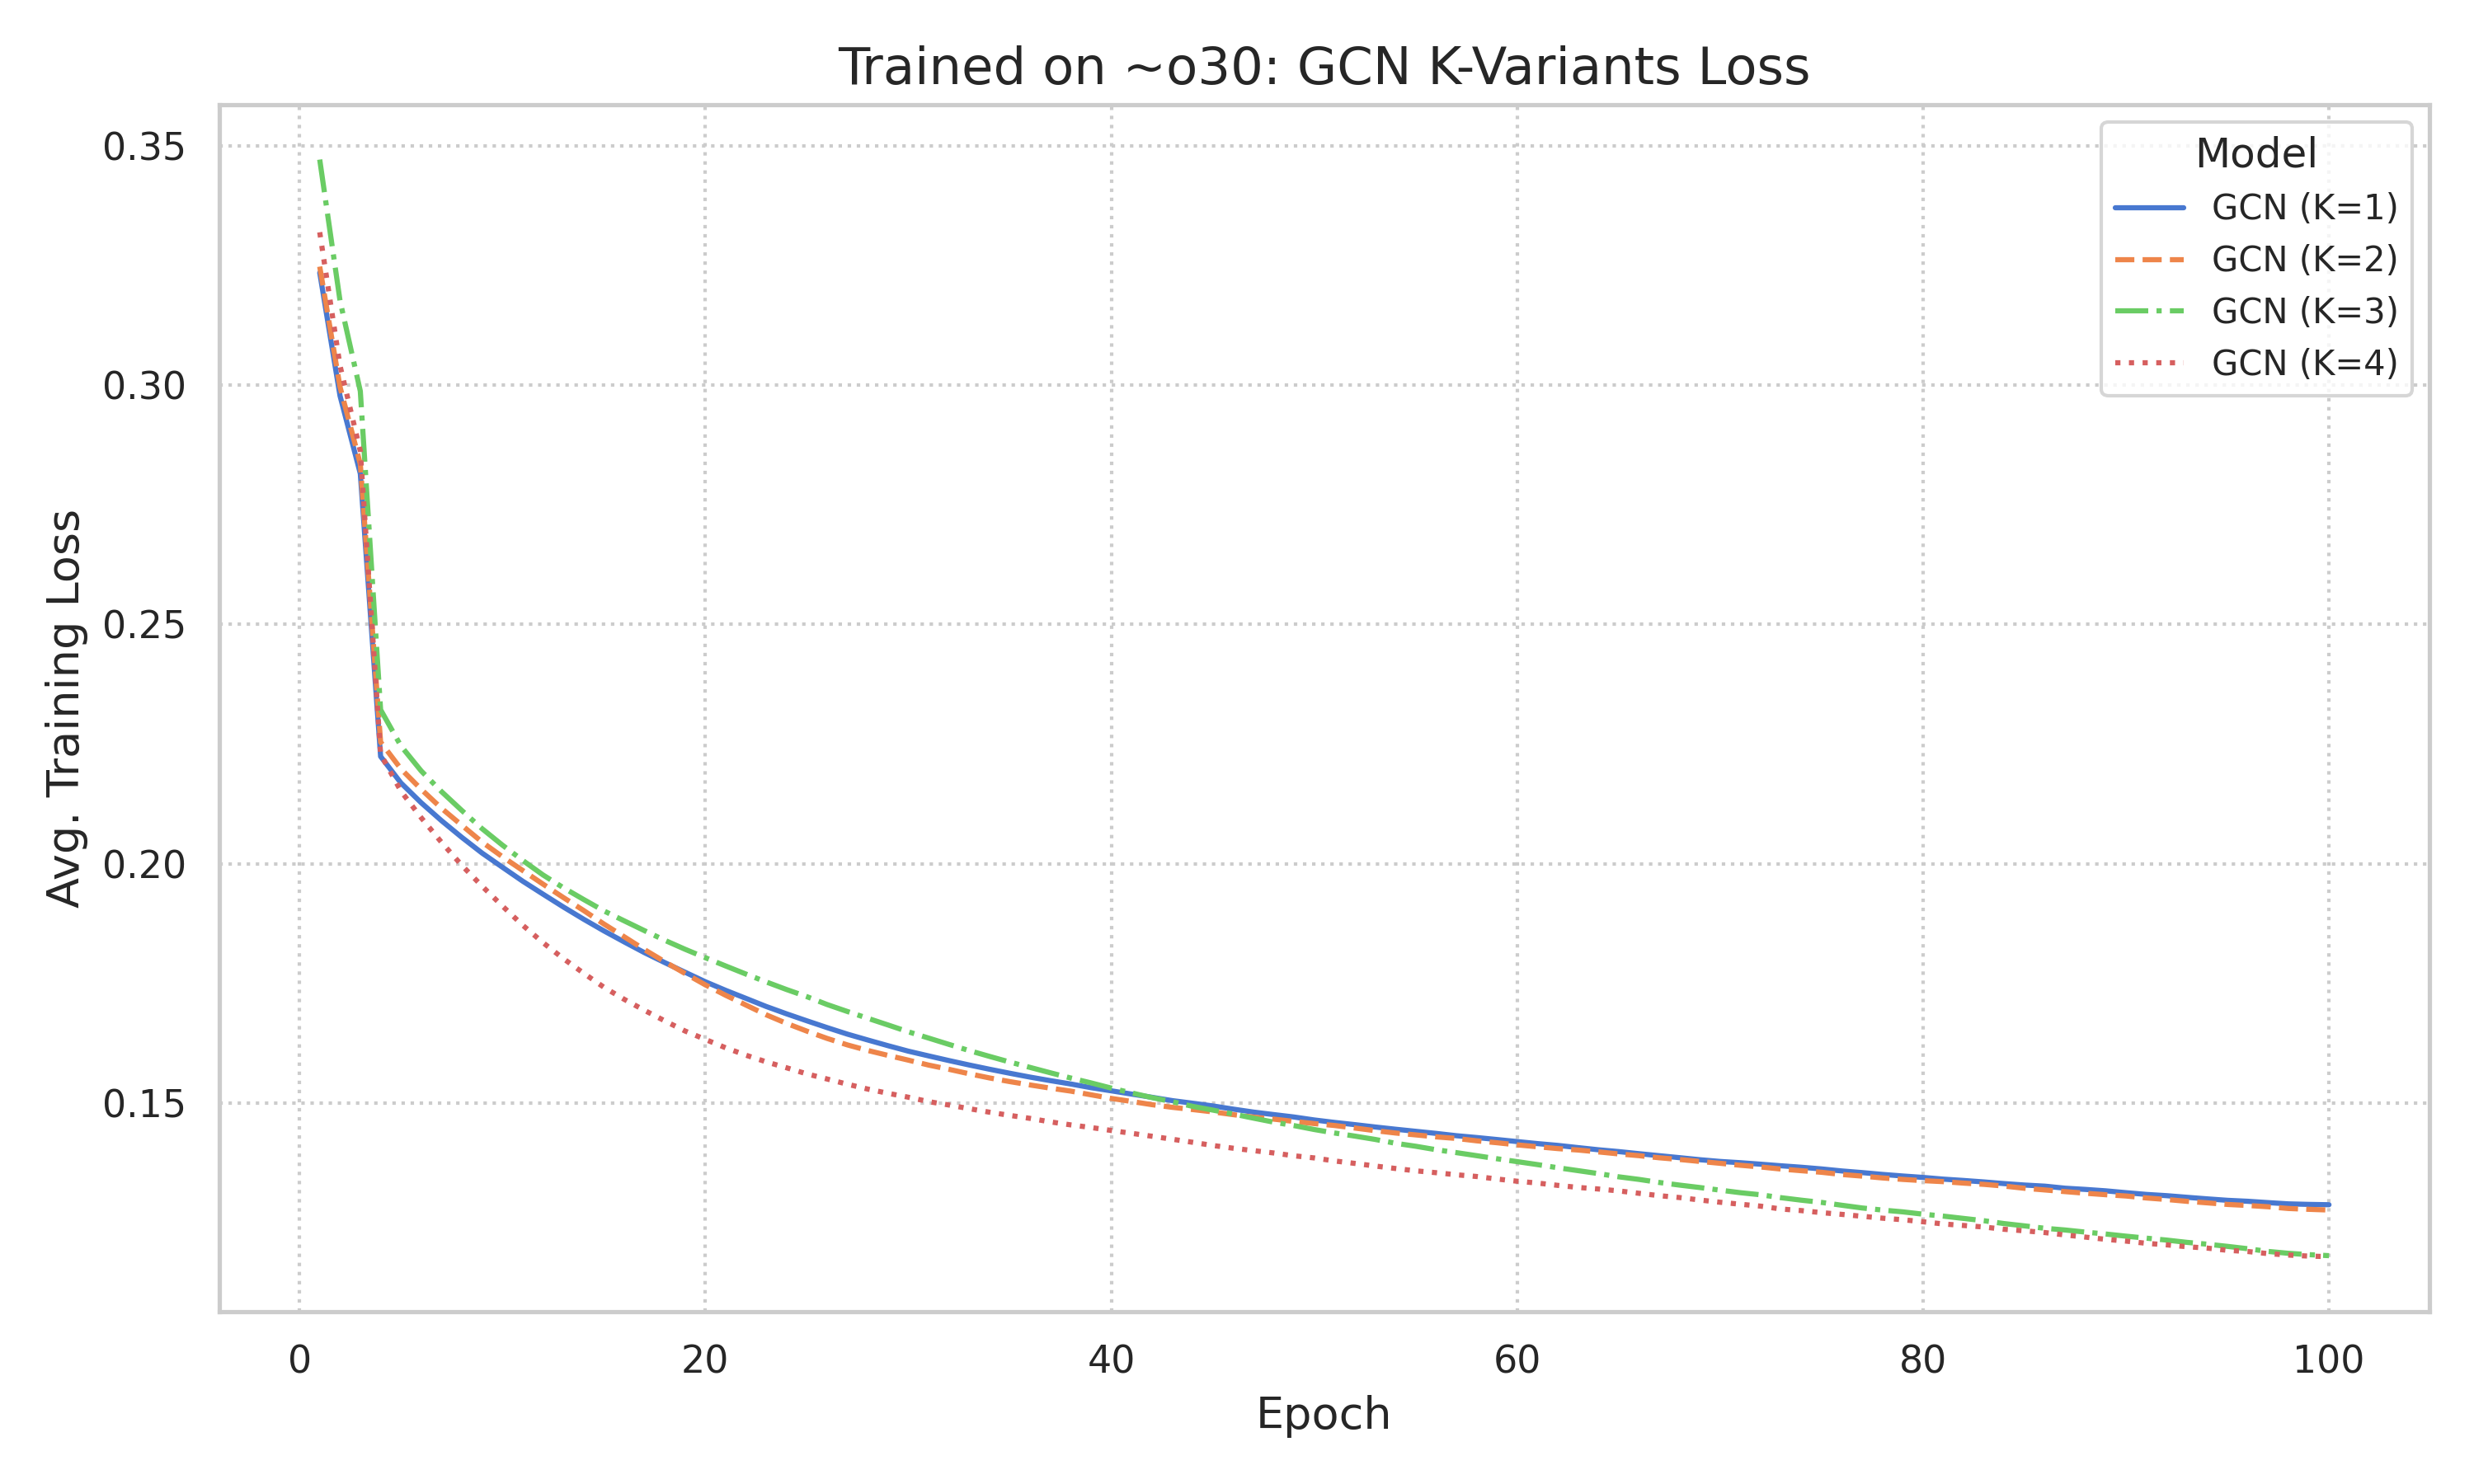
\includegraphics[width=\textwidth]{trainplotbase/TRAINED_ON_30_OBS/training_curves_focused/condition_o30/gcn_variants_train_loss.png} % UPDATE PATH
        \caption{GCN Variants: Training Loss (30\% Obst.)}
        \label{fig:gcn_train_loss_30obs}
    \end{subfigure}

    \vspace{0.3cm}

    % Row 3
    \begin{subfigure}[b]{0.48\textwidth}
        \centering
        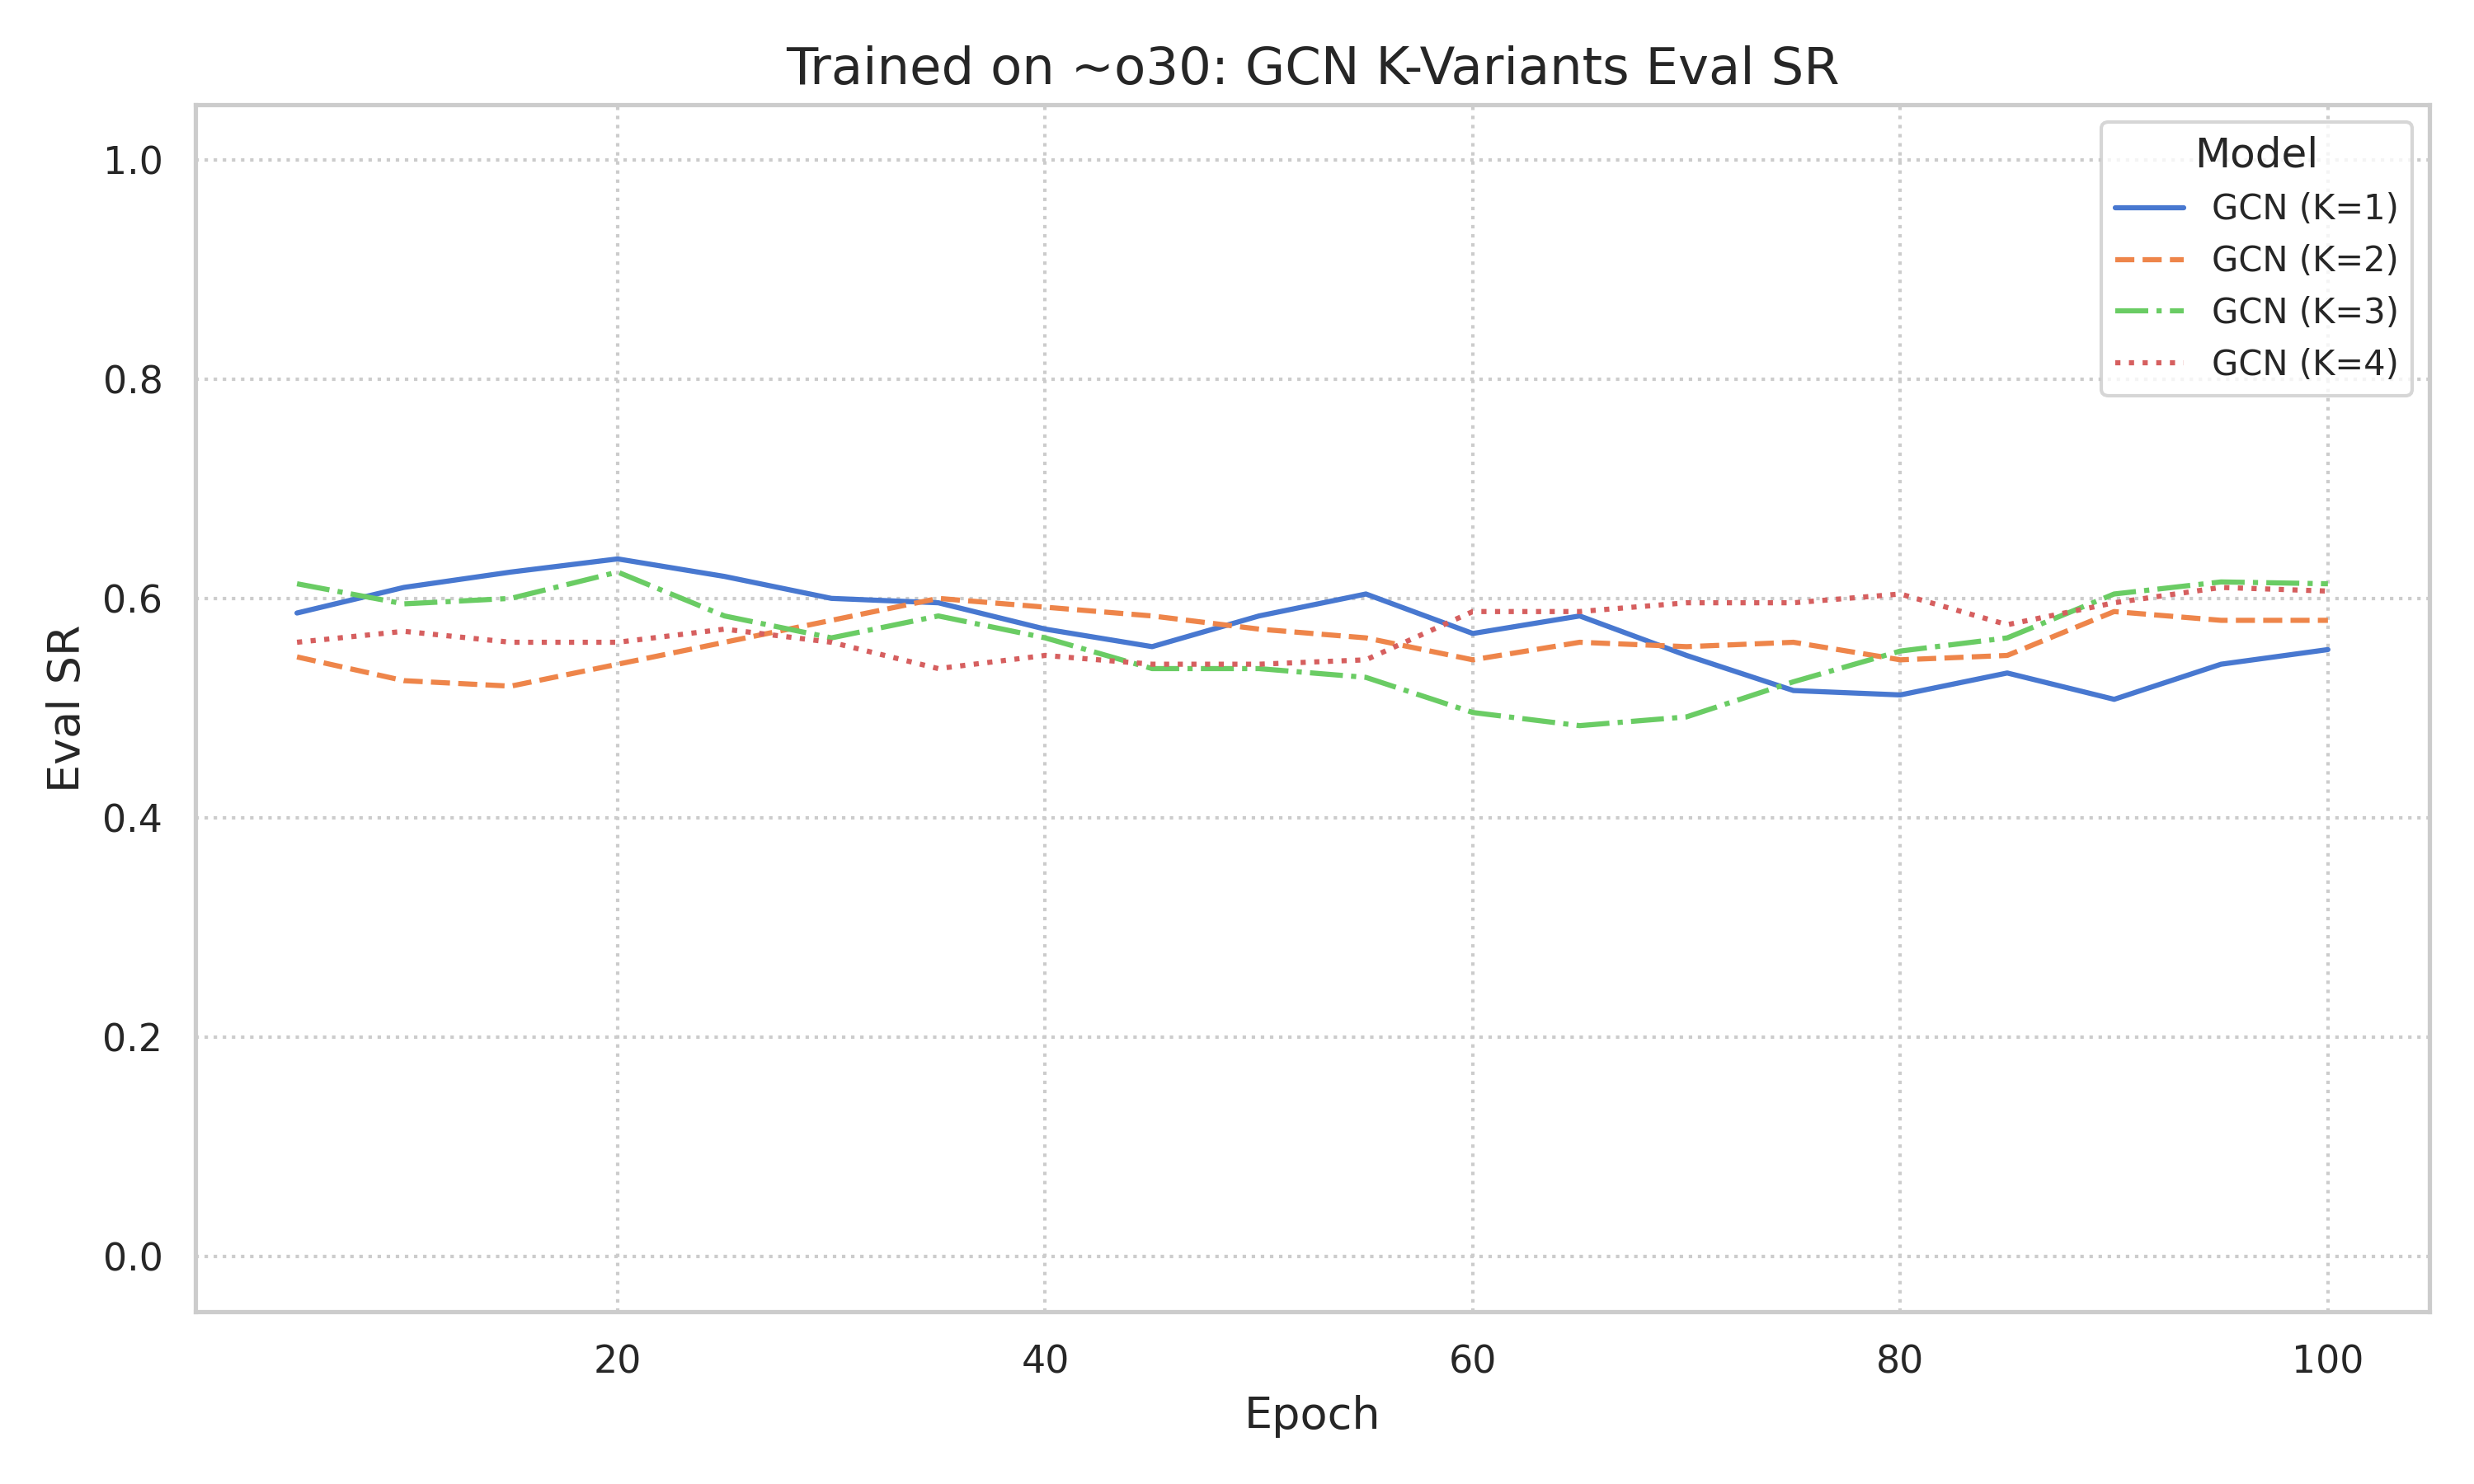
\includegraphics[width=\textwidth]{trainplotbase/TRAINED_ON_30_OBS/training_curves_focused/condition_o30/gcn_variants_eval_sr.png} % UPDATE PATH
        \caption{GCN Variants: Validation SR (30\% Obst.)}
        \label{fig:gcn_val_sr_30obs}
    \end{subfigure}
    \hfill
    \begin{subfigure}[b]{0.48\textwidth}
        \centering
        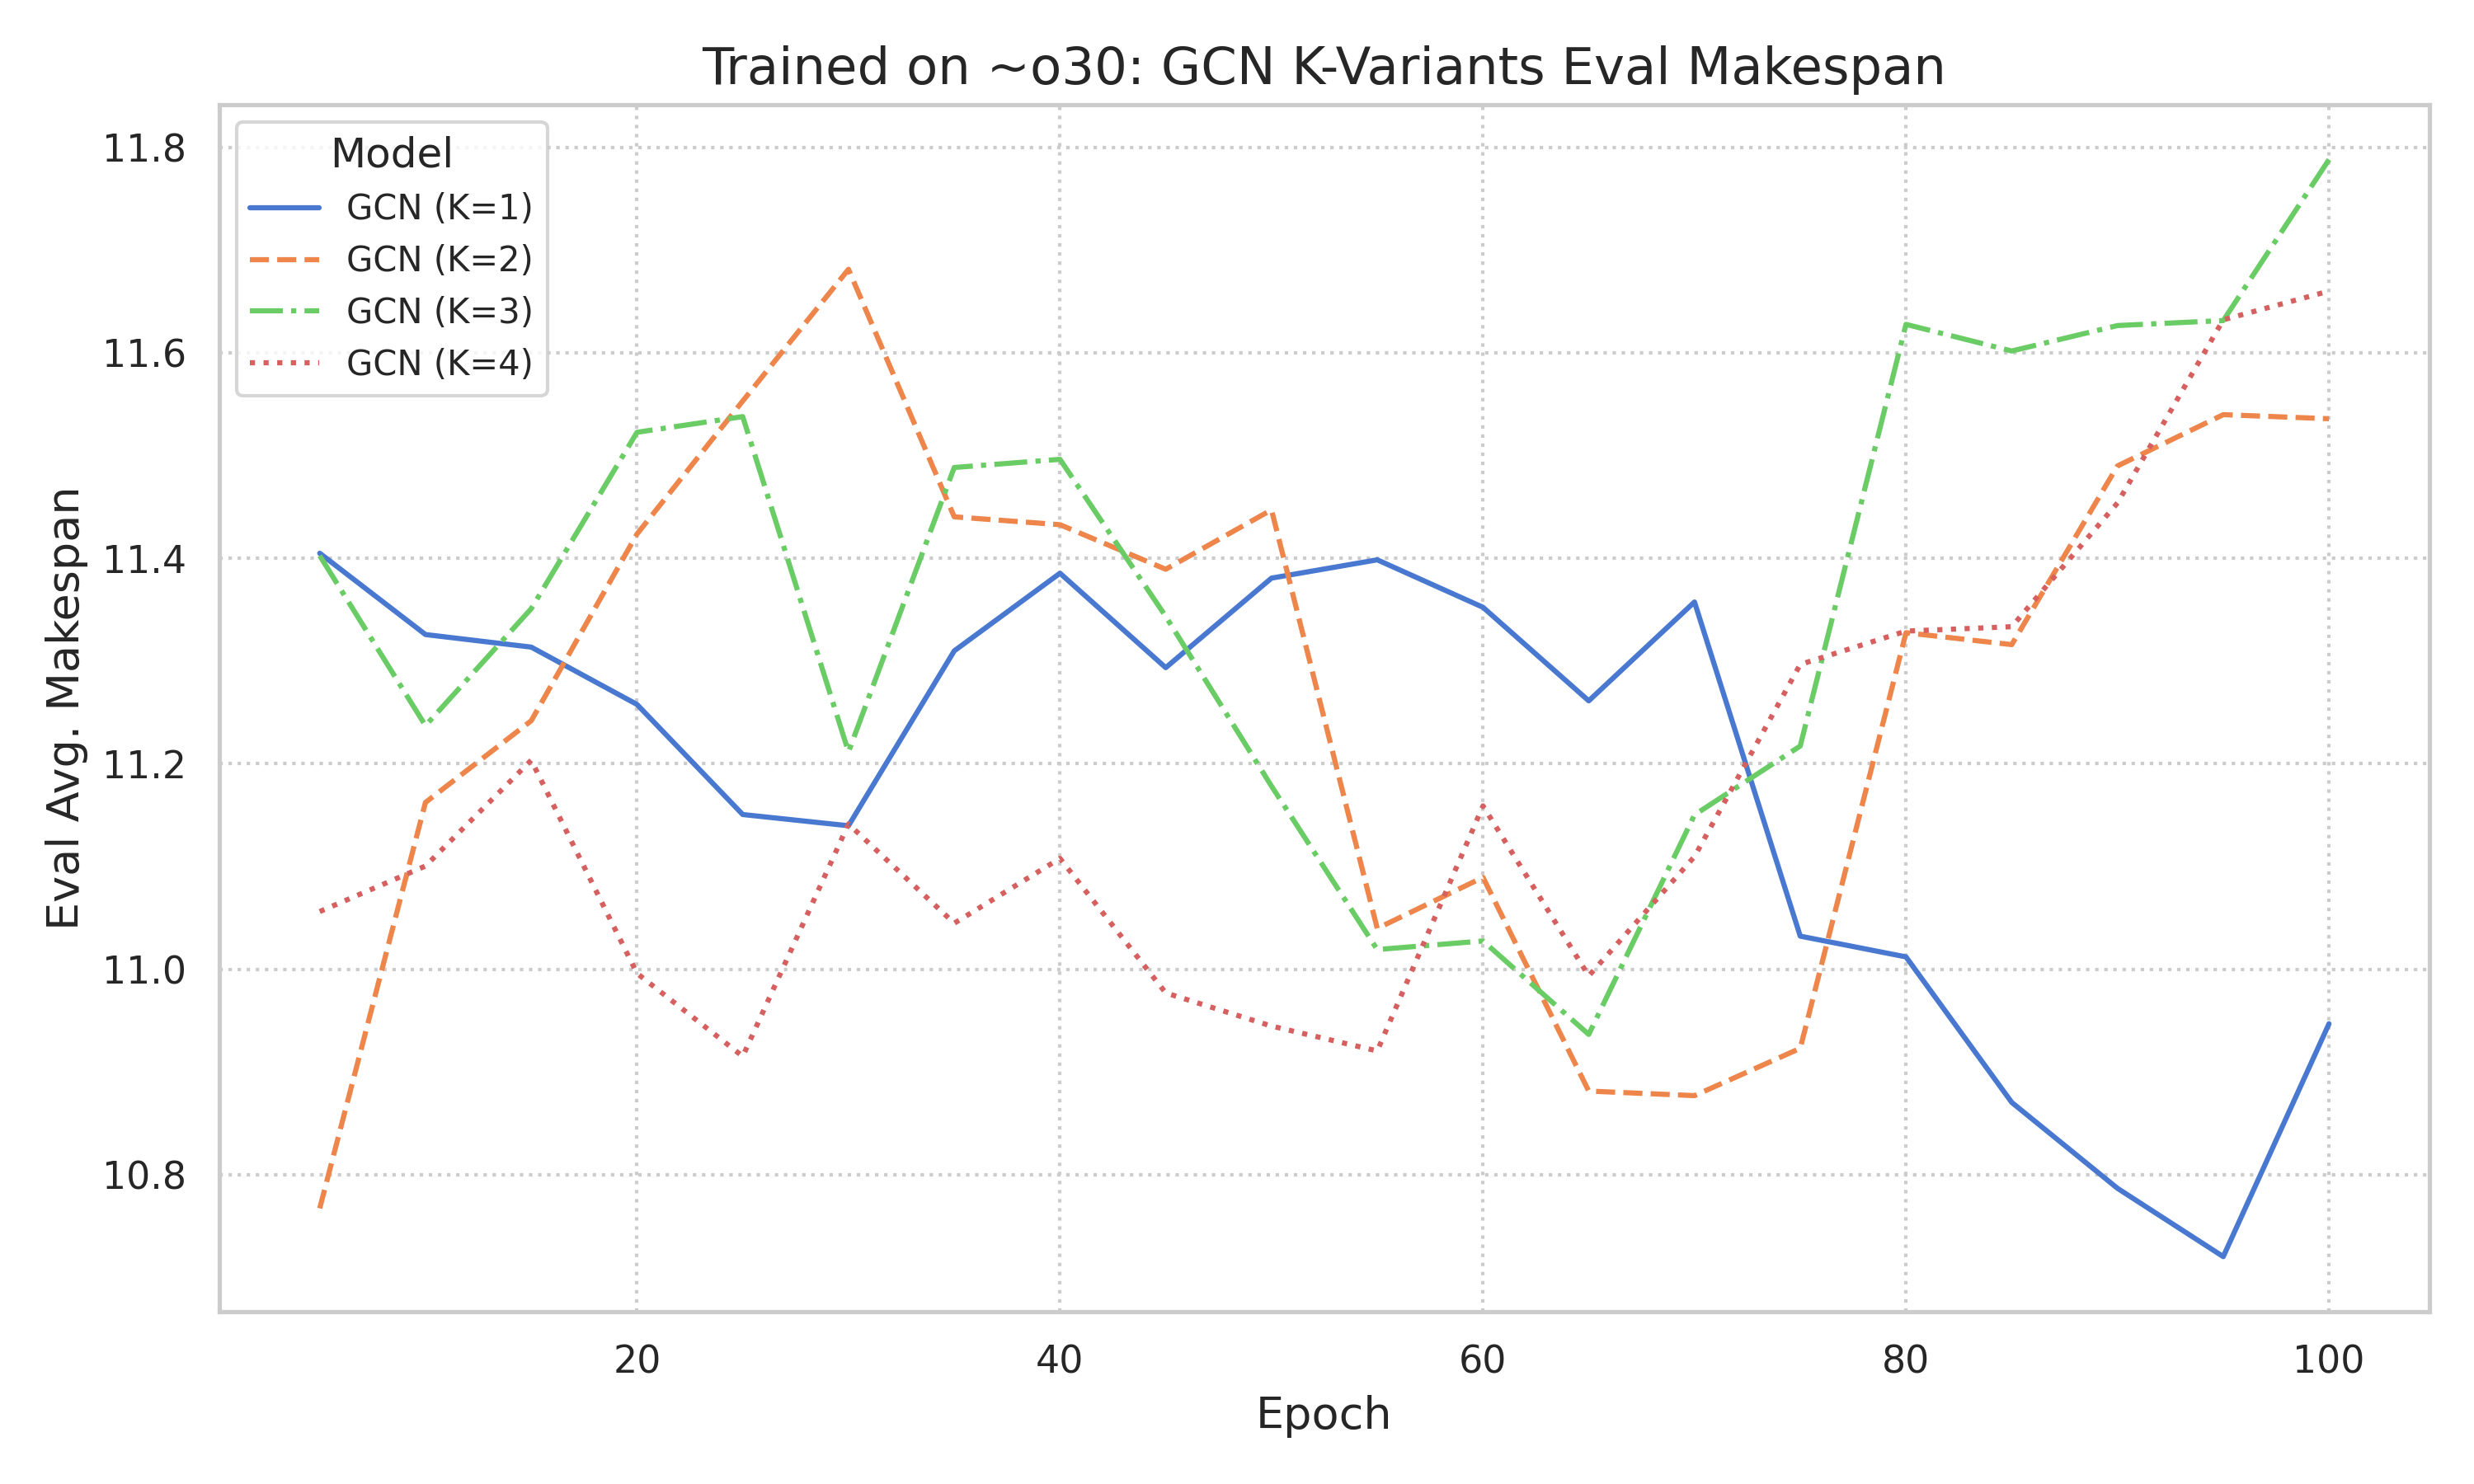
\includegraphics[width=\textwidth]{trainplotbase/TRAINED_ON_30_OBS/training_curves_focused/condition_o30/gcn_variants_eval_am.png} % UPDATE PATH
        \caption{GCN Variants: Validation AM (30\% Obst.)}
        \label{fig:gcn_val_am_30obs}
    \end{subfigure}

    \caption{Training progress for models trained on the 30\% obstacle density dataset. Layout and metrics are consistent with Figure~\ref{fig:training_curves_10obs_improved}.}
    \label{fig:training_curves_30obs_improved}
\end{figure}


\subsubsection{Summary of Training Dynamics:}
Across all training conditions (10\%, 20\%, and 30\% obstacle densities), the models demonstrated stable learning behavior. Training losses consistently decreased, while validation metrics (SR and AM) improved to a point of convergence, justifying the use of early stopping for model selection. The complexity of the training environment (i.e., obstacle density) influenced the absolute values of the achieved validation metrics and potentially the rate of convergence, but the overall learning process remained effective. The subsequent sections will delve into the quantitative performance of these trained models on unseen test data to assess their efficacy and generalization capabilities.
\section{Performance Across Varying Obstacle Densities}
\label{sec:perf_obstacle_density_detailed}
This section presents a detailed performance comparison of models trained on specific obstacle densities and then tested across all three densities (10\%, 20\%, 30\%). This helps in understanding both performance on matched train-test conditions and generalization to different environmental complexities.

\subsection{Models Trained on 10\% Obstacle Density (TrainSet-10D)}
\label{subsec:perf_10D_train_detailed}
Models were trained on the dataset with 10\% static obstacles. Their performance was then evaluated on test sets with 10\%, 20\%, and 30\% obstacle densities. Results are presented in Table \ref{tab:density_perf_10D_train}.

\begin{table}[htbp]
    \centering
    \caption{Performance on 10x10 Maps (5 Robots) with Varying Test Obstacle Densities. Models trained on 10\% Obstacles.}
    \label{tab:density_perf_10D_train}
    \scriptsize % For smaller font
    \begin{tabular}{llccccc}
        \toprule
        Test Density & Model & SR (\%) & AM & FT & Avg. Inf. Time (ms) & Params \\ % SR shown as %
        \midrule
        \multirow{7}{*}{10\%}
        & GCN (K=1) & 74.53 & 10.2972 & 65.5435 & 0.9750 & 39717 \\
        & GCN (K=2) & 80.95 & 10.4616 & 57.4741 & 0.9906 & 47909 \\
        & GCN (K=3) & 79.09 & 10.4084 & 59.9834 & 1.0092 & 56101 \\
        & GCN (K=4) & 80.43 & 10.5122 & 57.8810 & 1.0339 & 64293 \\
        & ADC-Main & 75.47 & 10.3443 & 64.0611 & 1.4841 & 39718 \\
        & \textbf{ADC-FixedT} & \textbf{81.16} & 10.5472 & \textbf{57.6398} & 1.4781 & 39717 \\
        & ADC-K1 & 76.50 & 10.3775 & 63.1387 & 0.9733 & 39718 \\
        \midrule
        \multirow{7}{*}{20\%}
        & GCN (K=1) & 50.87 & 10.3936 & 102.9569 & 0.6594 & 39717 \\
        & GCN (K=2) & 57.04 & 10.7347 & 95.0419 & 0.6795 & 47909 \\
        & GCN (K=3) & \textbf{58.21} & 10.7720 & \textbf{93.7835} & 0.6974 & 56101 \\
        & GCN (K=4) & 56.34 & 10.6921 & 95.7637 & 0.7143 & 64293 \\
        & ADC-Main & 55.88 & 10.6854 & 96.0687 & 1.1419 & 39718 \\
        & ADC-FixedT & 55.53 & 10.9518 & 97.8778 & 1.2411 & 39717 \\
        & ADC-K1 & 53.90 & 10.5032 & 99.1886 & 1.0532 & 39718 \\
        \midrule
        \multirow{7}{*}{30\%}
        & GCN (K=1) & 38.38 & 10.2595 & 132.1328 & 0.7271 & 39717 \\
        & GCN (K=2) & 36.93 & 10.3539 & 134.1203 & 0.9786 & 47909 \\
        & GCN (K=3) & 37.34 & 10.1833 & 133.9938 & 0.9951 & 56101 \\
        & GCN (K=4) & \textbf{39.42} & 10.4579 & 131.3320 & 1.0168 & 64293 \\
        & ADC-Main & \textbf{39.42} & 10.5947 & \textbf{130.0083} & 1.4707 & 39718 \\
        & ADC-FixedT & 39.21 & 10.8677 & 131.9917 & 1.4689 & 39717 \\
        & ADC-K1 & 35.68 & 10.1686 & 136.2614 & 1.1294 & 39718 \\
        \bottomrule
    \end{tabular}
\end{table}
When trained on 10\% obstacles:
\begin{itemize}
    \item \textbf{Testing on 10\% density (matched condition):} ADC-FixedT achieves the highest SR (81.16\%), slightly outperforming GCN K=2 (80.95\%) and GCN K=4 (80.43\%). ADC-Main (75.47\%) is competitive with GCN K=1 (74.53\%) but lower than other GCNs and ADC-FixedT.
    \item \textbf{Testing on 20\% density (generalization to higher density):} GCN K=3 shows the best SR (58.21\%). ADC-Main (55.88\%) performs comparably to GCN K=4 (56.34\%) and ADC-FixedT (55.53\%).
    \item \textbf{Testing on 30\% density (further generalization to higher density):} ADC-Main and GCN K=4 achieve the joint highest SR (39.42\%). ADC-Main also shows the best Flowtime (130.0083) in this challenging scenario.
\end{itemize}
The results suggest that when training on sparser environments, ADC-Main can match the best GCN's generalization to very dense environments, while a well-tuned ADC-FixedT can excel in matched conditions.

\subsection{Models Trained on 20\% Obstacle Density (TrainSet-20D)}
\label{subsec:perf_20D_train_detailed}
Models were trained on the dataset with 20\% static obstacles. Performance was evaluated on test sets with 10\%, 20\%, and 30\% obstacle densities. Results are in Table \ref{tab:density_perf_20D_train}.

\begin{table}[htbp]
    \centering
    \caption{Performance on 10x10 Maps (5 Robots) with Varying Test Obstacle Densities. Models trained on 20\% Obstacles.}
    \label{tab:density_perf_20D_train}
    \scriptsize % For smaller font
    \begin{tabular}{llccccc}
        \toprule
        Test Density & Model & SR (\%) & AM & FT & Avg. Inf. Time (ms) & Params \\
        \midrule
        \multirow{7}{*}{10\%}
        & GCN (K=1) & 74.22 & 10.3124 & 65.9400 & 0.9029 & 39717 \\
        & GCN (K=2) & 78.99 & 10.4325 & 60.6387 & 0.9870 & 47909 \\
        & GCN (K=3) & 77.74 & 10.5047 & 60.9731 & 1.0050 & 56101 \\
        & GCN (K=4) & 80.85 & 10.4571 & 57.7153 & 1.0295 & 64293 \\
        & ADC-Main & 77.12 & 10.2497 & 62.9959 & 1.4694 & 39718 \\
        & ADC-FixedT & \textbf{83.02} & 10.5673 & \textbf{55.7660} & 1.4701 & 39717 \\
        & ADC-K1 & 75.88 & 10.2906 & 64.0890 & 1.1215 & 39718 \\
        \midrule
        \multirow{7}{*}{20\%}
        & GCN (K=1) & 55.53 & 10.6059 & 96.7078 & 0.8863 & 39717 \\
        & GCN (K=2) & 62.17 & 10.9438 & 87.4098 & 0.9858 & 47909 \\
        & GCN (K=3) & 61.00 & 10.9351 & 89.3190 & 0.9985 & 56101 \\
        & GCN (K=4) & 61.93 & 10.8741 & 88.2037 & 1.0058 & 64293 \\
        & ADC-Main & 58.56 & 10.6998 & 92.4307 & 1.4283 & 39718 \\
        & ADC-FixedT & \textbf{64.61} & 11.3063 & \textbf{85.3679} & 1.4252 & 39717 \\ 
        & ADC-K1 & 59.25 & 10.6503 & 91.2980 & 1.0954 & 39718 \\
        \midrule
        \multirow{7}{*}{30\%}
        & GCN (K=1) & 44.40 & 10.7009 & 123.3195 & 0.9413 & 39717 \\
        & GCN (K=2) & 46.68 & 11.0267 & 121.5207 & 0.9631 & 47909 \\
        & GCN (K=3) & 44.19 & 10.6432 & 124.0249 & 0.6841 & 56101 \\
        & GCN (K=4) & \textbf{46.89} & 10.7124 & \textbf{120.6639} & 0.6937 & 64293 \\
        & ADC-Main & 43.98 & 10.7972 & 123.6888 & 1.1152 & 39718 \\
        & ADC-FixedT & 46.27 & 11.1300 & 121.4315 & 1.1141 & 39717 \\
        & ADC-K1 & 45.64 & 10.7364 & 121.3299 & 0.7984 & 39718 \\
        \bottomrule
    \end{tabular}
\end{table}
When trained on 20\% obstacles:
\begin{itemize}
    \item \textbf{Testing on 10\% density (generalization to lower density):} ADC-FixedT shows excellent generalization, achieving the highest SR (83.02\%) and best FT (55.7660), significantly outperforming GCN K=4 (SR 80.85\%). ADC-Main (77.12%) is also competitive.
    \item \textbf{Testing on 20\% density (matched condition):} ADC-FixedT again leads with an SR of 64.61\%, surpassing GCN K=2 (62.17\%). ADC-Main (58.56\%) is lower than the better GCNs in this case.
    \item \textbf{Testing on 30\% density (generalization to higher density):} GCN K=4 has the highest SR (46.89\%). ADC-FixedT (46.27\%) is very close, while ADC-Main (43.98\%) lags slightly.
\end{itemize}
Training on moderately dense environments seems to benefit ADC-FixedT, allowing it to perform well on both matched and sparser test cases.

\subsection{Models Trained on 30\% Obstacle Density (TrainSet-30D)}
\label{subsec:perf_30D_train_detailed}
Models were trained on the dataset with 30\% static obstacles. Performance was evaluated on test sets with 10\%, 20\%, and 30\% obstacle densities. Results are in Table \ref{tab:density_perf_30D_train}.

\begin{table}[htbp]
    \centering
    \caption{Performance on 10x10 Maps (5 Robots) with Varying Test Obstacle Densities. Models trained on 30\% Obstacles.}
    \label{tab:density_perf_30D_train}
    \scriptsize % For smaller font
    \begin{tabular}{llccccc}
        \toprule
        Test Density & Model & SR (\%) & AM & FT & Avg. Inf. Time (ms) & Params \\
        \midrule
        \multirow{7}{*}{10\%}
        & GCN (K=1) & 76.40 & 10.4024 & 62.8364 & 0.6742 & 39717 \\
        & GCN (K=2) & 77.02 & 10.4368 & 62.4255 & 0.6899 & 47909 \\
        & GCN (K=3) & 77.12 & 10.4940 & 62.9431 & 0.7104 & 56101 \\
        & GCN (K=4) & 77.43 & 10.5508 & 61.5280 & 0.7270 & 64293 \\
        & ADC-Main & 75.88 & 10.3915 & 63.5248 & 1.1517 & 39718 \\
        & ADC-FixedT & \textbf{81.47} & 10.6861 & \textbf{56.7008} & 1.1504 & 39717 \\
        & ADC-K1 & 76.29 & 10.4152 & 63.1925 & 0.8344 & 39718 \\
        \midrule
        \multirow{7}{*}{20\%}
        & GCN (K=1) & 58.44 & 10.6574 & 93.3946 & 0.6666 & 39717 \\
        & GCN (K=2) & 61.35 & 10.8121 & 89.6217 & 0.6868 & 47909 \\
        & GCN (K=3) & 60.42 & 11.0039 & 90.7392 & 0.7057 & 56101 \\
        & GCN (K=4) & 59.25 & 10.7603 & 91.7474 & 0.7233 & 64293 \\
        & ADC-Main & 59.02 & 10.7239 & 92.1409 & 1.1480 & 39718 \\
        & ADC-FixedT & \textbf{65.31} & 11.2531 & \textbf{84.8929} & 1.1463 & 39717 \\ 
        & ADC-K1 & 55.41 & 10.6176 & 97.0303 & 0.8273 & 39718 \\
        \midrule
        \multirow{7}{*}{30\%}
        & GCN (K=1) & 43.36 & 10.7273 & 125.0000 & 0.6658 & 39717 \\
        & GCN (K=2) & 44.19 & 10.8498 & 123.2988 & 0.6856 & 47909 \\
        & GCN (K=3) & 46.06 & 11.2387 & 120.5456 & 0.7035 & 56101 \\
        & GCN (K=4) & 47.10 & 10.5903 & 119.8278 & 0.7218 & 64293 \\
        & ADC-Main & 45.85 & 10.7059 & 121.3755 & 1.1448 & 39718 \\
        & ADC-FixedT & \textbf{47.51} & 11.3930 & \textbf{119.5456} & 1.1450 & 39717 \\
        & ADC-K1 & 45.02 & 10.7419 & 122.9979 & 0.8250 & 39718 \\
        \bottomrule
    \end{tabular}
\end{table}
When trained on 30\% obstacles:
\begin{itemize}
    \item \textbf{Testing on 10\% density (generalization to much lower density):} ADC-FixedT demonstrates remarkable generalization, achieving an SR of 81.47\%, significantly higher than the best GCN (K=4 at 77.43\%). ADC-Main (75.88\%) is comparable to the GCN baselines.
    \item \textbf{Testing on 20\% density (generalization to lower density):} ADC-FixedT again shows the best SR (65.31\%), outperforming GCN K=2 (61.35\%).
    \item \textbf{Testing on 30\% density (matched condition):} ADC-FixedT achieves the highest SR (47.51\%), slightly better than GCN K=4 (47.10\%). ADC-Main (45.85\%) is competitive.
\end{itemize}
Training on very dense environments (30\% obstacles) particularly highlights the strength of ADC-FixedT in generalizing to less cluttered scenarios. ADC-Main, while adaptive, doesn't consistently outperform the fixed variants in these generalization tasks.

\section{Ablation Studies}
\label{sec:ablation_studies_detailed}
To understand the contributions of different components of the ADC mechanism, we conducted ablation studies. The ADC-Main model uses a learnable diffusion time $t$ and a Taylor truncation order $K_{trunc}=10$. We compare it against:
\begin{itemize}
    \item \textbf{ADC-FixedT:} ADC with $K_{trunc}=10$ but $t$ is fixed (e.g., to a value like 1.0 or an empirically chosen default, not learned). This isolates the impact of learning $t$.
    \item \textbf{ADC-K1:} ADC with a learnable $t$ but $K_{trunc}=1$. This examines the effect of a very shallow diffusion approximation.
\end{itemize}
These ablations are compared against ADC-Main and the best performing GCN baseline. For this study, we focus on models trained on the 10\% obstacle density dataset (TrainSet-10D) and tested on the 10\% obstacle density test set, as this represents a matched condition where adaptive mechanisms might be expected to tune well.

\begin{table}[htbp]
    \centering
    \caption{Ablation Study Results (Test: 10x10 Map, 5 Robots, 10\% Obstacles). Models trained on 10\% Obstacles.}
    \label{tab:ablation}
    \scriptsize
    \begin{tabular}{lccccc}
        \toprule
        Model Variant (Trained on 10\% Obst.) & SR (\%) & AM & FT & Avg. Inf. Time (ms) & Params \\
        \midrule
        GCN (K=1) & 74.53 & 10.2972 & 65.5435 & 0.9750 & 39717 \\
        GCN (K=2) & 80.95 & 10.4616 & 57.4741 & 0.9906 & 47909 \\
        % GCN (K=3) & 79.09 & 10.4084 & 59.9834 & 1.0092 & 56101 \\
        GCN (K=4, Best Fixed-K overall) & 80.43 & 10.5122 & 57.8810 & 1.0339 & 64293 \\
        \midrule
        ADC-Main ($K_{trunc}$=10, learnable $t$) & 75.47 & 10.3443 & 64.0611 & 1.4841 & 39718 \\
        \textbf{ADC-FixedT ($K_{trunc}$=10, fixed $t$)} & \textbf{81.16} & 10.5472 & \textbf{57.6398} & 1.4781 & 39717 \\
        ADC-K1 ($K_{trunc}$=1, learnable $t$) & 76.50 & 10.3775 & 63.1387 & 0.9733 & 39718 \\
        \bottomrule
    \end{tabular}
\end{table}

Key observations from Table \ref{tab:ablation}:
\begin{itemize}
    \item \textbf{Impact of Learnable $t$ (ADC-Main vs. ADC-FixedT):} Surprisingly, for this specific train/test condition (10\% obstacles), ADC-FixedT (SR 81.16\%) outperforms ADC-Main (SR 75.47\%). This suggests that learning $t$ did not yield an advantage here, and a well-chosen fixed $t$ (perhaps close to an optimal value for this density) was more effective. The number of parameters is nearly identical (ADC-Main has one extra learnable scalar $t$).
    \item \textbf{Impact of Truncation Depth $K_{trunc}$ (ADC-Main vs. ADC-K1):} ADC-K1 (SR 76.50\%), which uses a very shallow diffusion ($K_{trunc}=1$), performs slightly better than ADC-Main (SR 75.47\%) and comparably to GCN K=1. This indicates that for this specific scenario, a deeper diffusion approximation (up to $K_{trunc}=10$) with a learnable $t$ did not provide significant benefits over a very localized one, or that the learned $t$ in ADC-Main might not have been optimal. ADC-K1 also has a much lower inference time than ADC-Main, comparable to GCN K=1, due to the minimal Taylor expansion.
    \item \textbf{Comparison with GCNs:} ADC-FixedT (SR 81.16\%) achieves the highest success rate among all models in this specific comparison, slightly surpassing GCN K=2 (80.95\%) and GCN K=4 (80.43\%).
\end{itemize}
These ablation results highlight that while ADC offers a theoretically appealing adaptive mechanism, its empirical benefits can be nuanced. The learnability of $t$ and the depth of diffusion ($K_{trunc}$) interact, and for certain matched train-test distributions, a simpler or well-tuned fixed configuration (like ADC-FixedT or even a simple GCN) can be highly effective. The sub-optimal performance of ADC-Main here might point to challenges in optimizing $t$ or the need for better initialization or regularization for $t$.

\section{Generalization Capability Across Obstacle Densities}
\label{sec:generalization_detailed}
A crucial aspect of a robust MRPP framework is its ability to generalize to environments with different characteristics from those seen during training. This section analyzes this capability by comparing models trained on one obstacle density and subsequently tested on others. We focus on scenarios where the training and testing obstacle densities differ, highlighting the performance of the best ADC variant against the strongest GCN baseline for each specific cross-density evaluation.

\subsection{Generalization from Low (10\%) to Higher Obstacle Densities}
\label{subsec:gen_low_to_high}
Models trained on the 10\% obstacle density dataset (TrainSet-10D) are evaluated on test sets with 20\% and 30\% obstacle densities. Performance is compared against the best GCN model (K=1 to K=4) specifically for that test density, using data from Table~\ref{tab:density_perf_10D_train}.

\begin{table}[htbp]
    \centering
    \caption{Generalization from 10\% Training Obstacles to Higher Test Densities (10x10 Map, 5 Robots). Best ADC variant from models trained on 10\% obstacles is selected for comparison.}
    \label{tab:gen_10D_to_high_revised}
    \scriptsize
    \begin{tabular}{llcccc}
        \toprule
        Tested On & Model (Trained on 10\% Obst.) & SR (\%) & AM & FT & SR Impr. over Best GCN (\%) \\
        \midrule
        \multirow{3}{*}{20\% Obstacles} % GCN K=3 (SR 58.21, AM 10.77, FT 93.78) is best GCN
        & GCN (K=3, Best GCN SR) & 58.21 & 10.7720 & 93.7835 & Baseline \\
        & ADC-Main & 55.88 & 10.6854 & 96.0687 & -4.00\% \\
        & ADC-FixedT & 55.53 & 10.9518 & 97.8778 & -4.60\% \\
        % & ADC-K1 & 53.90 & 10.5032 & 99.1886 & -7.40\% \\
        \midrule
        \multirow{3}{*}{30\% Obstacles} % GCN K=4 (SR 39.42, AM 10.45, FT 131.33) is best GCN
        & GCN (K=4, Best GCN SR) & 39.42 & 10.4579 & 131.3320 & Baseline \\
        & \textbf{ADC-Main (Best ADC)} & \textbf{39.42} & 10.5947 & \textbf{130.0083} & \textbf{0.00\%} \\
        & ADC-FixedT & 39.21 & 10.8677 & 131.9917 & -0.53\% \\
        % & ADC-K1 & 35.68 & 10.1686 & 136.2614 & -9.49\% \\
        \bottomrule
    \end{tabular}
\end{table}
Table \ref{tab:gen_10D_to_high_revised} details the generalization performance when training on 10\% obstacle density:
\begin{itemize}
    \item \textbf{Testing on 20\% density:} The best performing GCN model is GCN K=3 with an SR of 58.21\%. Among the ADC variants trained on 10\% obstacles, ADC-Main (SR 55.88\%) and ADC-FixedT (SR 55.53\%) perform slightly lower, with ADC-Main showing a 4.00\% relative decrease in SR compared to the best GCN.
    \item \textbf{Testing on 30\% density:} The best GCN model is GCN K=4 with an SR of 39.42\%. In this highly cluttered scenario, ADC-Main achieves the same SR (39.42\%) and offers a slightly better Flowtime (130.0083 vs. 131.3320 for GCN K=4), making it the best ADC performer and matching the top GCN.
\end{itemize}
When generalizing from sparse training environments to denser ones, the fixed-K GCNs often maintain strong performance. However, ADC-Main demonstrates an ability to match the best GCN in the most challenging high-density generalization task, indicating its potential for robustness in very cluttered, unseen conditions.

\subsection{Generalization from Medium (20\%) Obstacle Density}
\label{subsec:gen_medium_density}
Models trained on the 20\% obstacle density dataset (TrainSet-20D) are evaluated on test sets with 10\% (lower density) and 30\% (higher density) obstacles. Performance is compared against the best GCN model for each test density, using data from Table~\ref{tab:density_perf_20D_train}.

\begin{table}[htbp]
    \centering
    \caption{Generalization from 20\% Training Obstacles to Other Densities (10x10 Map, 5 Robots). Best ADC variant from models trained on 20\% obstacles is selected.}
    \label{tab:gen_20D_to_others_revised}
    \scriptsize
    \begin{tabular}{llcccc}
        \toprule
        Tested On & Model (Trained on 20\% Obst.) & SR (\%) & AM & FT & SR Impr. over Best GCN (\%) \\
        \midrule
        \multirow{2}{*}{10\% Obstacles} % GCN K=4 (SR 80.85, AM 10.45, FT 57.71) is best GCN
        & GCN (K=4, Best GCN SR) & 80.85 & 10.4571 & 57.7153 & Baseline \\
        & \textbf{ADC-FixedT (Best ADC)} & \textbf{83.02} & 10.5673 & \textbf{55.7660} & \textbf{+2.68\%} \\
        % & ADC-Main & 77.12 & 10.2497 & 62.9959 & -4.61\% \\
        \midrule
        \multirow{3}{*}{30\% Obstacles} % GCN K=4 (SR 46.89, AM 10.71, FT 120.66) is best GCN
        & GCN (K=4, Best GCN SR) & 46.89 & 10.7124 & 120.6639 & Baseline \\
        & ADC-FixedT (Best ADC) & 46.27 & 11.1300 & 121.4315 & -1.32\% \\
        & ADC-Main & 43.98 & 10.7972 & 123.6888 & -6.21\% \\
        % & ADC-K1 & 45.64 & 10.7364 & 121.3299 & -2.67\% \\
        \bottomrule
    \end{tabular}
\end{table}
Table \ref{tab:gen_20D_to_others_revised} shows the generalization from 20\% training density:
\begin{itemize}
    \item \textbf{Testing on 10\% density (to lower density):} ADC-FixedT (SR 83.02\%) demonstrates excellent generalization, outperforming the best GCN (K=4, SR 80.85\%) by +2.68\% in SR and also achieving better Flowtime.
    \item \textbf{Testing on 30\% density (to higher density):} GCN K=4 (SR 46.89\%) performs best. The best ADC variant here is ADC-FixedT (SR 46.27\%), which is very competitive but slightly lower, showing a -1.32\% relative SR difference.
\end{itemize}
Training on a medium-density environment allows ADC-FixedT to generalize effectively to sparser conditions. When generalizing to denser conditions, fixed-K GCNs can still be marginally stronger, but ADC-FixedT remains highly competitive.

\subsection{Generalization from High (30\%) to Lower Obstacle Densities}
\label{subsec:gen_high_to_low}
Models trained on the 30\% obstacle density dataset (TrainSet-30D) are evaluated on test sets with 10\% and 20% obstacle densities. Performance is compared against the best GCN model for each test density, using data from Table~\ref{tab:density_perf_30D_train}.

\begin{table}[htbp]
    \centering
    \caption{Generalization from 30\% Training Obstacles to Lower Test Densities (10x10 Map, 5 Robots). Best ADC variant from models trained on 30\% obstacles is selected.}
    \label{tab:gen_30D_to_low_revised}
    \scriptsize
    \begin{tabular}{llcccc}
        \toprule
        Tested On & Model (Trained on 30\% Obst.) & SR (\%) & AM & FT & SR Impr. over Best GCN (\%) \\
        \midrule
        \multirow{2}{*}{10\% Obstacles} % GCN K=4 (SR 77.43, AM 10.55, FT 61.52) is best GCN
        & GCN (K=4, Best GCN SR) & 77.43 & 10.5508 & 61.5280 & Baseline \\
        & \textbf{ADC-FixedT (Best ADC)} & \textbf{81.47} & 10.6861 & \textbf{56.7008} & \textbf{+5.22\%} \\
        % & ADC-Main & 75.88 & 10.3915 & 63.5248 & -2.00\% \\
        \midrule
        \multirow{2}{*}{20\% Obstacles} % GCN K=2 (SR 61.35, AM 10.81, FT 89.62) is best GCN
        & GCN (K=2, Best GCN SR) & 61.35 & 10.8121 & 89.6217 & Baseline \\
        & \textbf{ADC-FixedT (Best ADC)} & \textbf{65.31} & 11.2531 & \textbf{84.8929} & \textbf{+6.45\%} \\
        % & ADC-Main & 59.02 & 10.7239 & 92.1409 & -3.80\% \\
        \bottomrule
    \end{tabular}
\end{table}
Table \ref{tab:gen_30D_to_low_revised} highlights a key strength of the ADC approach when training in highly cluttered environments:
\begin{itemize}
    \item \textbf{Testing on 10\% density:} ADC-FixedT (SR 81.47\%) significantly outperforms the best GCN (K=4, SR 77.43\%), achieving a +5.22\% relative improvement in SR and notably better Flowtime. This indicates strong adaptation to much sparser conditions.
    \item \textbf{Testing on 20\% density:} ADC-FixedT (SR 65.31\%) again demonstrates superior generalization, outperforming GCN K=2 (SR 61.35\%) with a +6.45\% relative SR improvement and better Flowtime.
\end{itemize}
When models are trained on very dense and challenging environments (30\% obstacles), the ADC-FixedT variant consistently generalizes better to environments with lower obstacle densities compared to the best fixed-K GCNs. This suggests that the diffusion mechanism, even with a fixed $t$ learned or set from dense scenarios, offers a more robust representation for adapting to varying communication needs in less cluttered maps. The learnable ADC-Main, in this specific generalization direction (high-to-low density), did not perform as well as ADC-FixedT (referring to Table~\ref{tab:density_perf_30D_train}, ADC-Main SR was 75.88\% on 10\% test and 59.02\% on 20\% test when trained on 30\%), indicating that the fixed diffusion time derived from dense training was more beneficial for ADC-FixedT's generalization to sparser settings.

\subsubsection{Summary of Generalization Trends:}
The generalization capabilities depend on the direction of density shift:
\begin{itemize}
    \item \textbf{Low-to-High Density Generalization (e.g., Train 10\% $\rightarrow$ Test 30\%):} ADC-Main can match the best GCNs, showcasing robustness.
    \item \textbf{High-to-Low Density Generalization (e.g., Train 30\% $\rightarrow$ Test 10\%):} ADC-FixedT consistently outperforms GCNs, demonstrating significant adaptability.
    \item \textbf{Medium Density Training (Train 20\%):} ADC-FixedT generalizes well to lower densities, while GCNs are slightly better for higher densities, though ADC-FixedT remains competitive.
\end{itemize}
These findings suggest that the adaptive nature of the diffusion process, particularly with a well-suited (even if fixed) diffusion parameter, can lead to more robust policies across diverse environmental complexities compared to relying on a single fixed K-hop communication range.
\section{Comparative Analysis and Percentage Improvements}
\label{sec:comparative_analysis}
To summarize the benefits of ADC, we focus on scenarios where ADC variants (ADC-Main or ADC-FixedT) showed the best performance from Tables \ref{tab:density_perf_10D_train}, \ref{tab:density_perf_20D_train}, and \ref{tab:density_perf_30D_train}. We calculate the percentage improvement in Success Rate (SR) and Flowtime (FT) compared to the best performing GCN (K=1 to K=4) model in those specific scenarios. A positive percentage indicates improvement by ADC.

\begin{table}[htbp]
    \centering
    \caption{Summary of Best ADC Performance vs. Best GCN Baseline in Specific Scenarios}
    \label{tab:adc_vs_gcn_best_cases}
    \scriptsize
    \begin{tabular}{l l l c c c c}
        \toprule
        Training Density & Test Density & Best ADC Variant & ADC SR (\%) & Best GCN SR (\%) & SR Impr. (\%) & FT Impr. (\%) \\
        \midrule
        10\% & 10\% & ADC-FixedT & 81.16 & 80.95 (K=2) & +0.26\% & -0.25\% (vs K=2 FT 57.47) \\ % FT was 57.63 vs 57.47
        10\% & 30\% & ADC-Main & 39.42 & 39.42 (K=4) & 0.00\% & +0.99\% (vs K=4 FT 131.33) \\ % FT was 130.00 vs 131.33
        \midrule
        20\% & 10\% & ADC-FixedT & 83.02 & 80.85 (K=4) & +2.68\% & +3.38\% (vs K=4 FT 57.71) \\ % FT was 55.76 vs 57.71
        20\% & 20\% & ADC-FixedT & 64.61 & 62.17 (K=2) & +3.92\% & +2.34\% (vs K=2 FT 87.41) \\ % FT was 85.36 vs 87.41
        \midrule
        30\% & 10\% & ADC-FixedT & 81.47 & 77.43 (K=4) & +5.22\% & +7.85\% (vs K=4 FT 61.53) \\ % FT was 56.70 vs 61.53
        30\% & 20\% & ADC-FixedT & 65.31 & 61.35 (K=2) & +6.45\% & +5.28\% (vs K=2 FT 89.62) \\ % FT was 84.89 vs 89.62
        30\% & 30\% & ADC-FixedT & 47.51 & 47.10 (K=4) & +0.87\% & +0.23\% (vs K=4 FT 119.83) \\ % FT was 119.54 vs 119.83
        \bottomrule
    \end{tabular}
    \justify \scriptsize Note: SR Improvement is $((SR_{ADC} - SR_{GCN}) / SR_{GCN}) \times 100$. FT Improvement is $((FT_{GCN} - FT_{ADC}) / FT_{GCN}) \times 100$. Comparison is against the specific GCN-K variant that had the highest SR for that test case. ADC FT compared to that same GCN's FT.
\end{table}

Table \ref{tab:adc_vs_gcn_best_cases} highlights that:
\begin{itemize}
    \item ADC-FixedT consistently provides improvements, especially when generalizing from denser training environments to sparser test environments (e.g., Train 30\% $\rightarrow$ Test 10\% shows +5.22\% SR and +7.85\% FT improvement).
    \item Even in matched conditions (e.g., Train 20\% $\rightarrow$ Test 20\%), ADC-FixedT can offer tangible benefits (+3.92\% SR, +2.34\% FT).
    \item ADC-Main shows its strength in extremely cluttered generalization (Train 10\% $\rightarrow$ Test 30\%) by matching the best GCN in SR and slightly improving FT.
    \item The improvements in Flowtime often accompany or exceed SR improvements, indicating more efficient paths by the ADC variants when successful.
\end{itemize}
Overall, the ADC framework, particularly the ADC-FixedT variant, demonstrates a consistent ability to either match or outperform the best fixed-K GCNs across a range of conditions, with notable advantages in generalization scenarios. The learnable ADC-Main variant shows promise but might require further tuning or different training strategies to fully realize its potential across all scenarios compared to a well-chosen fixed $t$.

\section{Qualitative Analysis and Case Studies}
\label{sec:qualitative_analysis_detailed}

Quantitative metrics provide a broad overview of performance, but qualitative analysis of specific scenarios can offer deeper insights into the behavioral differences between the proposed ADC-enhanced framework and baseline GCN models. This section presents case studies to visualize and understand how adaptive communication can influence coordination and problem-solving in challenging multi-robot path planning situations.

\subsection{Case Study: Deadlock Resolution in a Congested Environment}
\label{subsec:case_study_deadlock}

To qualitatively assess the coordination capabilities of the different models, particularly in situations prone to deadlocks, a challenging scenario was selected from the test set. This case study involves a 10x10 grid environment with a moderate obstacle density. Five robots are required to navigate from their initial positions to their respective target goals. This specific configuration is designed to induce path conflicts and potential deadlocks, thereby highlighting differences in how the ADC-Main model and a strong GCN baseline (K=3) manage complex inter-agent interactions. Both models showcased here were trained on datasets with 10\% obstacle density. Figure~\ref{fig:case_study_deadlock_scenario} provides a visual comparison of their performance in this instance.

\begin{figure}[htbp]
    \centering
    % Ensure the figure environment spans the text width if needed
    % \begin{minipage}{\textwidth} % Optional: to group subfigures more tightly
    \begin{subfigure}[b]{0.32\textwidth}
        \centering
        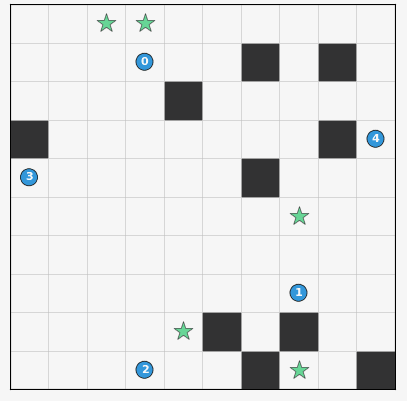
\includegraphics[width=\textwidth]{images/case_study_initial_state.png} % Replace with your actual image file
        \caption{Initial State: 5 Robots (circles) and their respective goals (stars).}
        \label{fig:cs_initial}
    \end{subfigure}
    \hfill % or \hspace{\fill}
    \begin{subfigure}[b]{0.32\textwidth}
        \centering
        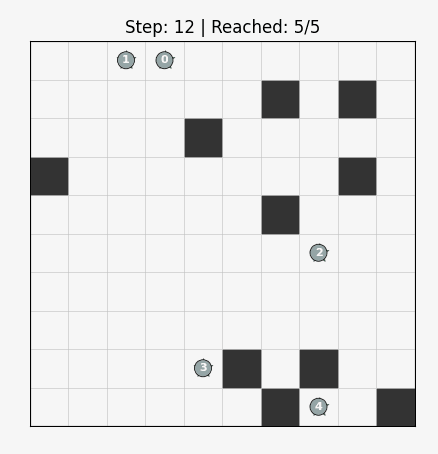
\includegraphics[width=\textwidth]{images/case_study_adc_success.png} % Replace with your actual image file
        \caption{ADC-Main: All 5 robots reached their goals in just 12 steps.}
        \label{fig:cs_adc_success}
    \end{subfigure}
    \hfill % or \hspace{\fill}
    \begin{subfigure}[b]{0.32\textwidth}
        \centering
        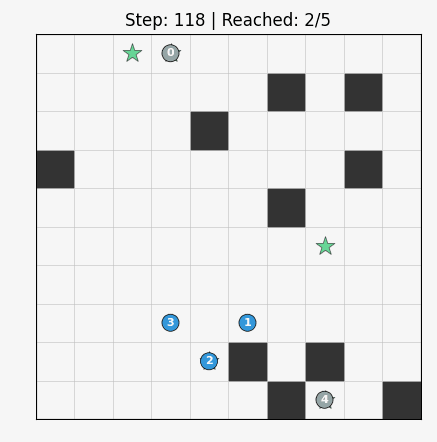
\includegraphics[width=\textwidth]{images/case_study_gcn_deadlock.png} % Replace with your actual image file
        \caption{GCN K=3: Only 2/5 robots reach by step 118; others in deadlock.}
        \label{fig:cs_gcn_deadlock}
    \end{subfigure}
    % \end{minipage}
    \caption{Case study comparing ADC-Main and GCN K=3 in a challenging scenario. (a) Shows the initial configuration of robots and goals. (b) Demonstrates ADC-Main successfully guiding all robots to their goals efficiently. (c) Illustrates GCN K=3 failing to resolve a deadlock situation for several robots even after many steps.}
    \label{fig:case_study_deadlock_scenario}
\end{figure}

\subsubsection{Scenario Description and Initial Configuration}
\label{subsubsec:scenario_description}

The initial state of the environment is presented in Figure~\ref{fig:cs_initial}. The key elements are:
\begin{itemize}
    \item \textbf{Environment:} A $10 \times 10$ grid with strategically placed static obstacles (black squares). These obstacles create narrow corridors and choke points, particularly in the central area and the lower-right quadrant.
    \item \textbf{Robots and Goals:} Five robots are present, depicted as light blue circles. Their corresponding goal locations are indicated by green stars.
        \begin{itemize}
            \item Robot 1 (Top-Left): Starts at approximately (1,2) (row, col from top-left, 0-indexed) and aims for a goal at (0,1).
            \item Robot 2 (Mid-Left): Starts at (4,0) and aims for a goal at (2,8) (top-right).
            \item Robot 3 (Center): Starts at (1,6) and aims for a goal at (4,4) (central).
            \item Robot 4 (Bottom-Left): Starts at (8,1) and aims for a goal at (6,3) (lower-left/central).
            \item Robot 5 (Bottom-Center): Starts at (6,6) and aims for a goal at (8,5) (bottom-center).
        \end{itemize}
    \item \textbf{Potential Conflict Zones:} The arrangement of starts, goals, and obstacles suggests several potential conflict zones:
        \begin{itemize}
            \item The narrow passage around (1,3)-(1,5) where Robot 1 and Robot 3 might interact.
            \item The central area around (4,4) which is Robot 3's goal and on a likely path for Robot 2.
            \item The lower-left and bottom-center regions where paths for Robots 4 and 5 are likely to intersect or require close coordination, especially given the proximity of their goals to obstacles.
        \end{itemize}
\end{itemize}
This setup is designed to test the models' ability to proactively coordinate and resolve complex multi-agent interactions to avoid collisions and prevent deadlocks.

\subsubsection{Performance of ADC-Main}
\label{subsubsec:adc_performance}
Figure~\ref{fig:cs_adc_success} illustrates the outcome when the ADC-Main model controls the robots.
\begin{itemize}
    \item \textbf{Outcome:} All five robots successfully navigated to their respective goal locations.
    \item \textbf{Efficiency:} The task was completed in a remarkably efficient manner, with all robots reaching their goals in just 12 time steps, as indicated in the top-left corner of the subfigure ("Step: 12 | Reached: 5/5").
    \item \textbf{Coordination:} The trajectories (implied by the final positions) suggest that the ADC-Main model effectively coordinated the robots. For instance, Robot 2 (now at (2,8)) appears to have navigated through the central area without conflicting with Robot 3 (now at (4,4)). Similarly, Robots 4 and 5 in the lower part of the grid have reached their goals without issue. The adaptive communication range learned by ADC likely allowed for more informed and proactive decision-making, enabling smoother path negotiation.
\end{itemize}

\subsubsection{Performance of GCN K=3 Baseline}
\label{subsubsec:gcn_performance}
Figure~\ref{fig:cs_gcn_deadlock} shows the state of the system when the GCN K=3 model is used.
\begin{itemize}
    \item \textbf{Outcome:} The GCN K=3 model failed to guide all robots to their goals. Only two out of the five robots (2/5) managed to reach their destinations.
    \item \textbf{Time Steps and Deadlock:} The subfigure shows the state at step 118 ("Step: 118 | Reached: 2/5"). Despite the significantly larger number of steps compared to ADC-Main, three robots remained stuck, indicating a deadlock situation.
        \begin{itemize}
            \item Robot 1 (at (0,1)) and Robot 2 (at (2,8)) successfully reached their goals.
            \item Robot 3 (near (1,6)), Robot 4 (near (8,1)), and Robot 5 (near (6,6)) appear to be in or near their initial positions or have made minimal progress, unable to resolve conflicts with each other or find clear paths around obstacles and other agents.
        \end{itemize}
    \item \textbf{Coordination Failure:} The fixed 3-hop communication range of the GCN K=3 model appears insufficient in this scenario to resolve the complex interactions, particularly for robots 3, 4, and 5. The limited information horizon may have prevented these robots from anticipating and avoiding the deadlock. For example, Robot 3's path to its central goal (4,4) is blocked by Robot 1, and its fixed communication range might not have allowed it to coordinate a yielding maneuver or find an alternative route effectively given Robot 2's trajectory.
\end{itemize}

\subsubsection{Comparative Analysis}
This case study highlights a significant difference in the emergent coordination behavior between the ADC-Main model and the GCN K=3 baseline. The ADC-Main model, with its ability to learn an appropriate diffusion radius for information sharing, demonstrated superior coordination, leading to an efficient, collision-free solution where all robots reached their goals. In contrast, the GCN K=3 model, constrained by its fixed communication neighborhood, struggled to resolve the inter-dependencies, resulting in a deadlock for a majority of the robots even after a prolonged period. This suggests that the adaptability in communication range afforded by ADC can be crucial for robust performance in congested multi-robot navigation tasks.



% \subsection{Analysis of Learned Diffusion Parameter $t$} % This section was already present
% \label{subsec:learned_t_detailed}
% ... (rest of your existing content for learned t) ...
\section{Computational Performance}
\label{sec:comp_perf_detailed}

\subsection{Inference Time}
\label{subsec:inference_time_detailed}
The average inference time per agent per step is crucial for real-time applicability. Table \ref{tab:inference_time_detailed} shows these times for models trained on 10\% obstacles and tested on the 10\% obstacle density test set.

\begin{table}[htbp]
    \centering
    \caption{Average Inference Time per Agent per Step (ms). Models trained on 10\% Obstacles, tested on 10\% density.}
    \label{tab:inference_time_detailed}
    \begin{tabular}{lc}
        \toprule
        Model & Avg. Inference Time (ms) \\
        \midrule
        GCN (K=1) & 0.9750 \\
        GCN (K=2) & 0.9906 \\
        GCN (K=3) & 1.0092 \\
        GCN (K=4) & 1.0339 \\
        \midrule
        ADC-Main ($K_{trunc}$=10) & 1.4841 \\
        ADC-FixedT ($K_{trunc}$=10) & 1.4781 \\
        ADC-K1 ($K_{trunc}$=1) & 0.9733 \\
        \bottomrule
    \end{tabular}
\end{table}
As observed in Table \ref{tab:inference_time_detailed}:
\begin{itemize}
    \item ADC-Main and ADC-FixedT (both with $K_{trunc}=10$) have higher inference times (approx. 1.48 ms) compared to GCN models (approx. 0.98-1.03 ms). This is expected due to the computation of Taylor series terms. The increase is about 43-52\% compared to GCN K=1.
    \item ADC-K1, with $K_{trunc}=1$, has an inference time (0.9733 ms) comparable to GCN K=1, as it involves minimal additional computation over a basic 1-hop GCN.
\end{itemize}
While ADC introduces some computational overhead, the inference times for all models are still very low, suggesting suitability for many real-time robotic applications where decision frequencies are in the order of tens or hundreds of milliseconds.
\begin{comment}
\subsection{Training Time}
\label{subsec:training_time_detailed}
The training time is another important practical consideration. While specific logs are not presented here, qualitatively:
\begin{itemize}
    \item ADC models (ADC-Main, ADC-FixedT with $K_{trunc}=10$) generally require more training time per epoch compared to GCN models. This is due to the forward pass computation of the Taylor series and the backward pass through these operations, especially when $t$ is also being learned.
    \item ADC-K1 would have training times closer to GCN K=1 due to its simpler aggregation.
    \item The overall training duration also depends on how quickly the models converge to good validation performance. If ADC models converge in fewer epochs to a better solution, the total training time might still be comparable or even favorable in some cases.
\end{itemize}
*(This section can be made more concrete if you have training time logs per epoch or total training times. A table similar to the commented-out one in your original file could be added here.)*

\end{comment}
\section{Chapter Summary}
\label{sec:results_summary_detailed}
The experimental results presented in this chapter provide a comprehensive evaluation of the ADC-enhanced MRPP framework.
Key findings include:
\begin{itemize}
    \item \textbf{Performance Variability:} The relative performance of ADC variants (ADC-Main, ADC-FixedT, ADC-K1) and fixed-K GCNs depends significantly on the specific training and testing conditions (obstacle densities). No single model universally dominates across all scenarios.
    \item \textbf{ADC-FixedT Strength:} The ADC-FixedT model, where the diffusion time $t$ is fixed but the diffusion mechanism is used, often emerged as a strong performer. It frequently matched or outperformed the best GCN baselines, especially in generalization tasks (e.g., training on high-density and testing on low-density, showing SR improvements of up to +6.45\%). This suggests that the diffusion process itself, even without a learnable $t$, can offer benefits in terms of smoothing and information propagation range.
    \item \textbf{ADC-Main (Learnable $t$):} The fully adaptive ADC-Main model, with a learnable $t$, showed competitive performance, particularly when generalizing from sparse training data to highly cluttered unseen environments (matching best GCN SR). However, it did not consistently outperform ADC-FixedT or the best GCNs across all conditions, indicating that the learning of $t$ might be challenging or that its benefits are more pronounced in specific types of environmental non-stationarity not fully captured here. The ablation studies also suggested that for matched 10\% density, a fixed $t$ or even a very shallow ADC ($K_{trunc}=1$) was more effective than ADC-Main with $K_{trunc}=10$.
    \item \textbf{Generalization:} ADC-FixedT demonstrated superior generalization when trained on high obstacle densities and tested on lower densities. Fixed-K GCNs sometimes generalized better from low to high densities.
    \item \textbf{Computational Cost:} ADC models with $K_{trunc}=10$ incur a moderate increase in inference time (around 40-50\% higher than GCNs) but remain viable for real-time application. Training times are also generally higher for deeper ADC models.
\end{itemize}
In conclusion, the adaptive diffusion concept holds promise for MRPP. While the fully learnable ADC-Main variant showed instances of good performance, the simpler ADC-FixedT often provided more consistent and significant improvements over GCNs, particularly in generalization. This suggests that the structure of diffusion itself is beneficial, and further research could focus on more robust methods for learning $t$, exploring different GSOs for $\mathbf{T}$, or dynamically scheduling $K_{trunc}$. The current findings pave the way for future investigations into more sophisticated adaptive communication strategies for multi-robot coordination.